\documentclass[twoside]{book}

% Packages required by doxygen
\usepackage{fixltx2e}
\usepackage{calc}
\usepackage{doxygen}
\usepackage[export]{adjustbox} % also loads graphicx
\usepackage{graphicx}
\usepackage[utf8]{inputenc}
\usepackage{makeidx}
\usepackage{multicol}
\usepackage{multirow}
\PassOptionsToPackage{warn}{textcomp}
\usepackage{textcomp}
\usepackage[nointegrals]{wasysym}
\usepackage[table]{xcolor}

% Font selection
\usepackage[T1]{fontenc}
\usepackage[scaled=.90]{helvet}
\usepackage{courier}
\usepackage{amssymb}
\usepackage{sectsty}
\renewcommand{\familydefault}{\sfdefault}
\allsectionsfont{%
  \fontseries{bc}\selectfont%
  \color{darkgray}%
}
\renewcommand{\DoxyLabelFont}{%
  \fontseries{bc}\selectfont%
  \color{darkgray}%
}
\newcommand{\+}{\discretionary{\mbox{\scriptsize$\hookleftarrow$}}{}{}}

% Page & text layout
\usepackage{geometry}
\geometry{%
  a4paper,%
  top=2.5cm,%
  bottom=2.5cm,%
  left=2.5cm,%
  right=2.5cm%
}
\tolerance=750
\hfuzz=15pt
\hbadness=750
\setlength{\emergencystretch}{15pt}
\setlength{\parindent}{0cm}
\setlength{\parskip}{3ex plus 2ex minus 2ex}
\makeatletter
\renewcommand{\paragraph}{%
  \@startsection{paragraph}{4}{0ex}{-1.0ex}{1.0ex}{%
    \normalfont\normalsize\bfseries\SS@parafont%
  }%
}
\renewcommand{\subparagraph}{%
  \@startsection{subparagraph}{5}{0ex}{-1.0ex}{1.0ex}{%
    \normalfont\normalsize\bfseries\SS@subparafont%
  }%
}
\makeatother

% Headers & footers
\usepackage{fancyhdr}
\pagestyle{fancyplain}
\fancyhead[LE]{\fancyplain{}{\bfseries\thepage}}
\fancyhead[CE]{\fancyplain{}{}}
\fancyhead[RE]{\fancyplain{}{\bfseries\leftmark}}
\fancyhead[LO]{\fancyplain{}{\bfseries\rightmark}}
\fancyhead[CO]{\fancyplain{}{}}
\fancyhead[RO]{\fancyplain{}{\bfseries\thepage}}
\fancyfoot[LE]{\fancyplain{}{}}
\fancyfoot[CE]{\fancyplain{}{}}
\fancyfoot[RE]{\fancyplain{}{\bfseries\scriptsize Generated by Doxygen }}
\fancyfoot[LO]{\fancyplain{}{\bfseries\scriptsize Generated by Doxygen }}
\fancyfoot[CO]{\fancyplain{}{}}
\fancyfoot[RO]{\fancyplain{}{}}
\renewcommand{\footrulewidth}{0.4pt}
\renewcommand{\chaptermark}[1]{%
  \markboth{#1}{}%
}
\renewcommand{\sectionmark}[1]{%
  \markright{\thesection\ #1}%
}

% Indices & bibliography
\usepackage{natbib}
\usepackage[titles]{tocloft}
\setcounter{tocdepth}{3}
\setcounter{secnumdepth}{5}
\makeindex

% Hyperlinks (required, but should be loaded last)
\usepackage{ifpdf}
\ifpdf
  \usepackage[pdftex,pagebackref=true]{hyperref}
\else
  \usepackage[ps2pdf,pagebackref=true]{hyperref}
\fi
\hypersetup{%
  colorlinks=true,%
  linkcolor=blue,%
  citecolor=blue,%
  unicode%
}

% Custom commands
\newcommand{\clearemptydoublepage}{%
  \newpage{\pagestyle{empty}\cleardoublepage}%
}

\usepackage{caption}
\captionsetup{labelsep=space,justification=centering,font={bf},singlelinecheck=off,skip=4pt,position=top}

%===== C O N T E N T S =====

\begin{document}

% Titlepage & ToC
\hypersetup{pageanchor=false,
             bookmarksnumbered=true,
             pdfencoding=unicode
            }
\pagenumbering{alph}
\begin{titlepage}
\vspace*{7cm}
\begin{center}%
{\Large Information Gathering Library }\\
\vspace*{1cm}
{\large Generated by Doxygen 1.8.13}\\
\end{center}
\end{titlepage}
\clearemptydoublepage
\pagenumbering{roman}
\tableofcontents
\clearemptydoublepage
\pagenumbering{arabic}
\hypersetup{pageanchor=true}

%--- Begin generated contents ---
\chapter{Anytime Information Acquisition}
\label{index}\hypertarget{index}{}This respository accompanies the 2018 R\+AL paper\+: \href{http://ieeexplore.ieee.org/document/8260881/}{\tt http\+://ieeexplore.\+ieee.\+org/document/8260881/}. This work considers the problem of planning trajectories for a team of mobile robots that efficiently gather information about a target process of interest. In this simulation, a number of mobile robots following a unicycle motion model with discretized motion primitives, aim to track the evolution of a number of moving targets following a double-\/integrator model driven by Gaussian noise. The algorithm is implemented in C++, and the simulation can be configured to run from the command line with C++, or with Python via Py\+Bind11 for visualization of the simulation environment.

\subsection*{Dependencies}

Ensure that the following dependencies are installed\+:


\begin{DoxyItemize}
\item Eigen3
\item Yaml-\/\+C\+PP
\item Pybind11
\item C\+G\+AL
\end{DoxyItemize}

\subsection*{Compilation}

\begin{DoxyVerb}cd <install_location>
mkdir build && cd build
cmake ..
make
cd ..
\end{DoxyVerb}


\subsection*{Example Usage in C++}

Experiments can be run using C++ or M\+A\+T\+L\+AB. In C++, the configuration for the robot starting locations, sensing model, and other parameters is done in data/init\+\_\+info\+\_\+planner\+\_\+\+S\+E2.\+yaml. C\+SV files containing the resulting data are generated in the results folder.

The code can be executed\+: \begin{DoxyVerb}build/bin/test_info_planner_SE2 data/init_info_planner_ARVI.yaml
\end{DoxyVerb}


\subsection*{Usage in Python}

Note\+: Currently plotting is only supported for single robots.

Run the following script\+: \begin{DoxyVerb}python script/python/pyInfo.py
\end{DoxyVerb}


To change the scenario file, edit the python script parameters import, i.\+e. \begin{DoxyVerb}params = IG.Parameters('data/init_info_planner_ARVI.yaml')
\end{DoxyVerb}


To point to the desired simulation configuration to run.

\subsection*{Immediate To-\/\+Do\textquotesingle{}s}


\begin{DoxyItemize}
\item Clean up the way that Coordinate Descent Planning is implemented, e.\+g. by wrapping the A\+R\+VI Planner into a new Planner that takes in a team of Robots, rather than the user having to manage the Coordinate Descent algorithm themselves.
\item Clean up the Target Model interface to neatly handle multiple targets, data association, and retrieval of belief states.
\item Fix Python Plotting code to work for Multiple Robots
\item Clean up State Space / E\+NV representation to allow for motion primitives on S\+E(3), and define distance metrics on the Pose types themselves, for cleaner usage in R\+VI / A\+R\+VI delta-\/crossing.
\item Add support for Drawing obstacle maps in 2D
\item Longer Term\+: Make Python plotting code for 3D environments..
\end{DoxyItemize}

\section*{Future Features to be supported}


\begin{DoxyItemize}
\item Robots and targets are both general \textquotesingle{}Agents\textquotesingle{}, which can have a full state space in S\+E(3). Robots can hold a belief (target) model, for any agents whose pose they wish to estimate (including itself). This model can be converted by the planner into a Linear Gaussian model, and used for target tracking.
\item The above means each state Space must be convertible to S\+E(3), and vice versa. Either S\+E(3) should be the baseline, and we project down into lower spaces for control, or the other spaces exist and we lift into S\+E(3) for generic operations on the robot state. I vote for making everything S\+E(3) and projecting into lower spaces for control.
\item Come up with a good interface for what an Agent is, and what traits it posesses. I.\+e. robot has a state Space (S\+E(3)), an action space (on some subspace of S\+E(3)), one or more sensors, a planner, which generates a trajectory, and a controller to follow the trajectory.
\item We should include drivers for the sensors in the Sensor package, which interface between hardware and the Sensor models we have, i.\+e. Gazebo / real L\+I\+D\+AR or camera into our camera or range and bearing sensors.
\item A R\+OS wrapper which can allow us to wrap robot topics and sensors from Gazebo into the appropriate pieces of our module.
\item Software should be modular and split into packages that are easy to pull in, and maintained in a repository. I.\+e. Estimation, planning, Base (robots and state spaces perhaps).
\item Scenario files. The programming task could ultimately be reduced to a user writing a new scenario file. To accomplish a particular task, the user will configure the robots and sensors appropriately, then call the appropriate planner for the scenario.
\end{DoxyItemize}

\section*{R\+OS Wrapper}


\begin{DoxyItemize}
\item Create a Node that maps appropriate R\+OS topics into the inputs and outputs of the regular node. (D\+O\+NE)
\item What topics does this node subscribe to? For each robot in the team, it subscribes to a position, i.\+e. nav\+\_\+msgs/odom type. (D\+O\+NE)
\item Right now this is a centralized planner, so spawning the planner will have to remap topics for all robots into this node. (D\+O\+NE)
\item This should publish output velocity commands to some node, which will be remapped as determined by the simulation. (D\+O\+NE)
\item Other world parameters needed are the map for collision checking. The remaining parameters are planner specific, or related to the robot dynamics. (D\+O\+NE)
\item Later on, this will also subscribe to sensors in order to estimate the target. But for the very first iteration, this will be a static target with a fixed location provided by R\+OS parameters. 
\end{DoxyItemize}
\chapter{Hierarchical Index}
\section{Class Hierarchy}
This inheritance list is sorted roughly, but not completely, alphabetically\+:\begin{DoxyCompactList}
\item \contentsline{section}{nx\+:\+:compare\+\_\+cov}{\pageref{structnx_1_1compare__cov}}{}
\item \contentsline{section}{nx\+:\+:compare\+\_\+pair$<$ infostate $>$}{\pageref{structnx_1_1compare__pair}}{}
\item \contentsline{section}{nx\+:\+:compare\+\_\+pair\+\_\+info$<$ infostate $>$}{\pageref{structnx_1_1compare__pair__info}}{}
\item \contentsline{section}{Y\+A\+ML\+:\+:convert$<$ std\+:\+:array$<$ TP, S\+I\+ZE $>$ $>$}{\pageref{structYAML_1_1convert_3_01std_1_1array_3_01TP_00_01SIZE_01_4_01_4}}{}
\item \contentsline{section}{nx\+:\+:D$<$ state $>$}{\pageref{structnx_1_1D}}{}
\item \contentsline{section}{nx\+:\+:Environment$<$ state $>$}{\pageref{classnx_1_1Environment}}{}
\item \contentsline{section}{nx\+:\+:Environment$<$ S\+E3\+Pose $>$}{\pageref{classnx_1_1Environment}}{}
\begin{DoxyCompactList}
\item \contentsline{section}{nx\+:\+:S\+E2\+Environment}{\pageref{classnx_1_1SE2Environment}}{}
\end{DoxyCompactList}
\item exception\begin{DoxyCompactList}
\item \contentsline{section}{nx\+:\+:S\+E3\+Pose\+:\+:Invalid\+Orientation}{\pageref{classnx_1_1SE3Pose_1_1InvalidOrientation}}{}
\end{DoxyCompactList}
\item \contentsline{section}{nx\+:\+:Gaussian\+Belief}{\pageref{structnx_1_1GaussianBelief}}{}
\item \contentsline{section}{nx\+:\+:Info\+Planner\+A\+R\+VI$<$ state $>$}{\pageref{classnx_1_1InfoPlannerARVI}}{}
\item \contentsline{section}{nx\+:\+:Info\+State$<$ state $>$}{\pageref{structnx_1_1InfoState}}{}
\item \contentsline{section}{nx\+:\+:Info\+State\+Space$<$ state $>$}{\pageref{structnx_1_1InfoStateSpace}}{}
\item \contentsline{section}{nx\+:\+:Kalman\+Filter}{\pageref{classnx_1_1KalmanFilter}}{}
\item \contentsline{section}{nx\+:\+:Logger}{\pageref{classnx_1_1Logger}}{}
\item \contentsline{section}{nx\+:\+:map\+\_\+nd}{\pageref{classnx_1_1map__nd}}{}
\item \contentsline{section}{nx\+:\+:Measurement}{\pageref{structnx_1_1Measurement}}{}
\item \contentsline{section}{nx\+:\+:Motion\+Primitive$<$ state, control $>$}{\pageref{structnx_1_1MotionPrimitive}}{}
\item \contentsline{section}{nx\+:\+:Multi\+Target\+Filter$<$ state $>$}{\pageref{classnx_1_1MultiTargetFilter}}{}
\item \contentsline{section}{nx\+:\+:normal\+\_\+random\+\_\+variable}{\pageref{structnx_1_1normal__random__variable}}{}
\item \contentsline{section}{nx\+:\+:Parameters}{\pageref{classnx_1_1Parameters}}{}
\item \contentsline{section}{nx\+:\+:Planner\+Output$<$ state $>$}{\pageref{structnx_1_1PlannerOutput}}{}
\item \contentsline{section}{nx\+:\+:Probability}{\pageref{classnx_1_1Probability}}{}
\item \contentsline{section}{nx\+:\+:Robot$<$ state $>$}{\pageref{classnx_1_1Robot}}{}
\item \contentsline{section}{nx\+:\+:S\+E3\+Pose}{\pageref{structnx_1_1SE3Pose}}{}
\item \contentsline{section}{nx\+:\+:Sensor$<$ state $>$}{\pageref{classnx_1_1Sensor}}{}
\item \contentsline{section}{nx\+:\+:Parameters\+:\+:System\+Model}{\pageref{structnx_1_1Parameters_1_1SystemModel}}{}
\item \contentsline{section}{nx\+:\+:Target}{\pageref{structnx_1_1Target}}{}
\begin{DoxyCompactList}
\item \contentsline{section}{nx\+:\+:Info\+Target}{\pageref{structnx_1_1InfoTarget}}{}
\end{DoxyCompactList}
\item \contentsline{section}{nx\+:\+:Target\+Model}{\pageref{classnx_1_1TargetModel}}{}
\begin{DoxyCompactList}
\item \contentsline{section}{nx\+:\+:Info\+Target\+Model}{\pageref{classnx_1_1InfoTargetModel}}{}
\end{DoxyCompactList}
\end{DoxyCompactList}

\chapter{Class Index}
\section{Class List}
Here are the classes, structs, unions and interfaces with brief descriptions\+:\begin{DoxyCompactList}
\item\contentsline{section}{\hyperlink{structnx_1_1compare__cov}{nx\+::compare\+\_\+cov} }{\pageref{structnx_1_1compare__cov}}{}
\item\contentsline{section}{\hyperlink{structnx_1_1compare__pair}{nx\+::compare\+\_\+pair$<$ infostate $>$} }{\pageref{structnx_1_1compare__pair}}{}
\item\contentsline{section}{\hyperlink{structnx_1_1compare__pair__info}{nx\+::compare\+\_\+pair\+\_\+info$<$ infostate $>$} }{\pageref{structnx_1_1compare__pair__info}}{}
\item\contentsline{section}{\hyperlink{structYAML_1_1convert_3_01std_1_1array_3_01TP_00_01SIZE_01_4_01_4}{Y\+A\+M\+L\+::convert$<$ std\+::array$<$ T\+P, S\+I\+Z\+E $>$ $>$} }{\pageref{structYAML_1_1convert_3_01std_1_1array_3_01TP_00_01SIZE_01_4_01_4}}{}
\item\contentsline{section}{\hyperlink{structnx_1_1D}{nx\+::\+D$<$ state $>$} }{\pageref{structnx_1_1D}}{}
\item\contentsline{section}{\hyperlink{classnx_1_1Environment}{nx\+::\+Environment$<$ state $>$} }{\pageref{classnx_1_1Environment}}{}
\item\contentsline{section}{\hyperlink{structnx_1_1GaussianBelief}{nx\+::\+Gaussian\+Belief} }{\pageref{structnx_1_1GaussianBelief}}{}
\item\contentsline{section}{\hyperlink{classnx_1_1InfoPlannerARVI}{nx\+::\+Info\+Planner\+A\+R\+V\+I$<$ state $>$} }{\pageref{classnx_1_1InfoPlannerARVI}}{}
\item\contentsline{section}{\hyperlink{structnx_1_1InfoState}{nx\+::\+Info\+State$<$ state $>$} }{\pageref{structnx_1_1InfoState}}{}
\item\contentsline{section}{\hyperlink{structnx_1_1InfoStateSpace}{nx\+::\+Info\+State\+Space$<$ state $>$} }{\pageref{structnx_1_1InfoStateSpace}}{}
\item\contentsline{section}{\hyperlink{structnx_1_1InfoTarget}{nx\+::\+Info\+Target} }{\pageref{structnx_1_1InfoTarget}}{}
\item\contentsline{section}{\hyperlink{classnx_1_1InfoTargetModel}{nx\+::\+Info\+Target\+Model} }{\pageref{classnx_1_1InfoTargetModel}}{}
\item\contentsline{section}{\hyperlink{classnx_1_1SE3Pose_1_1InvalidOrientation}{nx\+::\+S\+E3\+Pose\+::\+Invalid\+Orientation} }{\pageref{classnx_1_1SE3Pose_1_1InvalidOrientation}}{}
\item\contentsline{section}{\hyperlink{classnx_1_1KalmanFilter}{nx\+::\+Kalman\+Filter} }{\pageref{classnx_1_1KalmanFilter}}{}
\item\contentsline{section}{\hyperlink{classnx_1_1Logger}{nx\+::\+Logger} }{\pageref{classnx_1_1Logger}}{}
\item\contentsline{section}{\hyperlink{classnx_1_1map__nd}{nx\+::map\+\_\+nd} }{\pageref{classnx_1_1map__nd}}{}
\item\contentsline{section}{\hyperlink{structnx_1_1Measurement}{nx\+::\+Measurement} }{\pageref{structnx_1_1Measurement}}{}
\item\contentsline{section}{\hyperlink{structnx_1_1MotionPrimitive}{nx\+::\+Motion\+Primitive$<$ state, control $>$} }{\pageref{structnx_1_1MotionPrimitive}}{}
\item\contentsline{section}{\hyperlink{classnx_1_1MultiTargetFilter}{nx\+::\+Multi\+Target\+Filter$<$ state $>$} }{\pageref{classnx_1_1MultiTargetFilter}}{}
\item\contentsline{section}{\hyperlink{structnx_1_1normal__random__variable}{nx\+::normal\+\_\+random\+\_\+variable} }{\pageref{structnx_1_1normal__random__variable}}{}
\item\contentsline{section}{\hyperlink{classnx_1_1Parameters}{nx\+::\+Parameters} }{\pageref{classnx_1_1Parameters}}{}
\item\contentsline{section}{\hyperlink{structnx_1_1PlannerOutput}{nx\+::\+Planner\+Output$<$ state $>$} }{\pageref{structnx_1_1PlannerOutput}}{}
\item\contentsline{section}{\hyperlink{classnx_1_1Probability}{nx\+::\+Probability} }{\pageref{classnx_1_1Probability}}{}
\item\contentsline{section}{\hyperlink{classnx_1_1Robot}{nx\+::\+Robot$<$ state $>$} }{\pageref{classnx_1_1Robot}}{}
\item\contentsline{section}{\hyperlink{classnx_1_1SE2Environment}{nx\+::\+S\+E2\+Environment} }{\pageref{classnx_1_1SE2Environment}}{}
\item\contentsline{section}{\hyperlink{structnx_1_1SE3Pose}{nx\+::\+S\+E3\+Pose} }{\pageref{structnx_1_1SE3Pose}}{}
\item\contentsline{section}{\hyperlink{classnx_1_1Sensor}{nx\+::\+Sensor$<$ state $>$} }{\pageref{classnx_1_1Sensor}}{}
\item\contentsline{section}{\hyperlink{structnx_1_1Parameters_1_1SystemModel}{nx\+::\+Parameters\+::\+System\+Model} }{\pageref{structnx_1_1Parameters_1_1SystemModel}}{}
\item\contentsline{section}{\hyperlink{structnx_1_1Target}{nx\+::\+Target} }{\pageref{structnx_1_1Target}}{}
\item\contentsline{section}{\hyperlink{classnx_1_1TargetModel}{nx\+::\+Target\+Model} }{\pageref{classnx_1_1TargetModel}}{}
\end{DoxyCompactList}

\chapter{Class Documentation}
\hypertarget{structnx_1_1compare__cov}{}\section{nx\+:\+:compare\+\_\+cov Struct Reference}
\label{structnx_1_1compare__cov}\index{nx\+::compare\+\_\+cov@{nx\+::compare\+\_\+cov}}
\subsection*{Public Member Functions}
\begin{DoxyCompactItemize}
\item 
\mbox{\Hypertarget{structnx_1_1compare__cov_ae631418a3c019ed7e215a777c855337c}\label{structnx_1_1compare__cov_ae631418a3c019ed7e215a777c855337c}} 
bool {\bfseries operator()} (const std\+::pair$<$ double, Matrix\+Xd $>$ \&p1, const std\+::pair$<$ double, Matrix\+Xd $>$ \&p2) const
\end{DoxyCompactItemize}


The documentation for this struct was generated from the following file\+:\begin{DoxyCompactItemize}
\item 
include/igl/planning/infoplanner\+\_\+arvi.\+h\end{DoxyCompactItemize}

\hypertarget{structnx_1_1compare__pair}{}\section{nx\+:\+:compare\+\_\+pair$<$ infostate $>$ Struct Template Reference}
\label{structnx_1_1compare__pair}\index{nx\+::compare\+\_\+pair$<$ infostate $>$@{nx\+::compare\+\_\+pair$<$ infostate $>$}}
\subsection*{Public Member Functions}
\begin{DoxyCompactItemize}
\item 
\mbox{\Hypertarget{structnx_1_1compare__pair_aa41844bf701ea83514d86853433898e2}\label{structnx_1_1compare__pair_aa41844bf701ea83514d86853433898e2}} 
bool {\bfseries operator()} (const std\+::pair$<$ double, std\+::shared\+\_\+ptr$<$ infostate $>$$>$ \&p1, const std\+::pair$<$ double, std\+::shared\+\_\+ptr$<$ infostate $>$$>$ \&p2) const
\end{DoxyCompactItemize}


The documentation for this struct was generated from the following file\+:\begin{DoxyCompactItemize}
\item 
include/igl/planning/infoplanner\+\_\+arvi.\+h\end{DoxyCompactItemize}

\hypertarget{structnx_1_1compare__pair__info}{}\section{nx\+:\+:compare\+\_\+pair\+\_\+info$<$ infostate $>$ Struct Template Reference}
\label{structnx_1_1compare__pair__info}\index{nx\+::compare\+\_\+pair\+\_\+info$<$ infostate $>$@{nx\+::compare\+\_\+pair\+\_\+info$<$ infostate $>$}}
\subsection*{Public Member Functions}
\begin{DoxyCompactItemize}
\item 
\mbox{\Hypertarget{structnx_1_1compare__pair__info_aa7ce05b866a5ee5b9045b9a141299a14}\label{structnx_1_1compare__pair__info_aa7ce05b866a5ee5b9045b9a141299a14}} 
bool {\bfseries operator()} (const std\+::pair$<$ double, std\+::shared\+\_\+ptr$<$ infostate $>$$>$ \&p1, const std\+::pair$<$ double, std\+::shared\+\_\+ptr$<$ infostate $>$$>$ \&p2) const
\end{DoxyCompactItemize}


The documentation for this struct was generated from the following file\+:\begin{DoxyCompactItemize}
\item 
include/igl/planning/infoplanner\+\_\+arvi.\+h\end{DoxyCompactItemize}

\hypertarget{structYAML_1_1convert_3_01std_1_1array_3_01TP_00_01SIZE_01_4_01_4}{}\section{Y\+A\+ML\+:\+:convert$<$ std\+:\+:array$<$ TP, S\+I\+ZE $>$ $>$ Struct Template Reference}
\label{structYAML_1_1convert_3_01std_1_1array_3_01TP_00_01SIZE_01_4_01_4}\index{Y\+A\+M\+L\+::convert$<$ std\+::array$<$ T\+P, S\+I\+Z\+E $>$ $>$@{Y\+A\+M\+L\+::convert$<$ std\+::array$<$ T\+P, S\+I\+Z\+E $>$ $>$}}
\subsection*{Static Public Member Functions}
\begin{DoxyCompactItemize}
\item 
\mbox{\Hypertarget{structYAML_1_1convert_3_01std_1_1array_3_01TP_00_01SIZE_01_4_01_4_a1eeed03353acfe9bd2a8c97a8904f498}\label{structYAML_1_1convert_3_01std_1_1array_3_01TP_00_01SIZE_01_4_01_4_a1eeed03353acfe9bd2a8c97a8904f498}} 
static Node {\bfseries encode} (const std\+::array$<$ TP, S\+I\+ZE $>$ \&rhs)
\item 
\mbox{\Hypertarget{structYAML_1_1convert_3_01std_1_1array_3_01TP_00_01SIZE_01_4_01_4_ae3cd9a7f90106511270f06bde606c427}\label{structYAML_1_1convert_3_01std_1_1array_3_01TP_00_01SIZE_01_4_01_4_ae3cd9a7f90106511270f06bde606c427}} 
static bool {\bfseries decode} (const Node \&node, std\+::array$<$ TP, S\+I\+ZE $>$ \&rhs)
\end{DoxyCompactItemize}


The documentation for this struct was generated from the following file\+:\begin{DoxyCompactItemize}
\item 
include/igl/utils/yaml\+\_\+addon.\+h\end{DoxyCompactItemize}

\hypertarget{structnx_1_1D}{}\section{nx\+:\+:D$<$ state $>$ Struct Template Reference}
\label{structnx_1_1D}\index{nx\+::\+D$<$ state $>$@{nx\+::\+D$<$ state $>$}}
\subsection*{Public Member Functions}
\begin{DoxyCompactItemize}
\item 
void \hyperlink{structnx_1_1D_af2c0c3653af6d84d9977ae110e1688cf}{operator()} (\hyperlink{structnx_1_1InfoState}{Info\+State}$<$ state $>$ $\ast$p) const
\end{DoxyCompactItemize}


\subsection{Member Function Documentation}
\mbox{\Hypertarget{structnx_1_1D_af2c0c3653af6d84d9977ae110e1688cf}\label{structnx_1_1D_af2c0c3653af6d84d9977ae110e1688cf}} 
\index{nx\+::D@{nx\+::D}!operator()@{operator()}}
\index{operator()@{operator()}!nx\+::D@{nx\+::D}}
\subsubsection{\texorpdfstring{operator()()}{operator()()}}
{\footnotesize\ttfamily template$<$class state $>$ \\
void \hyperlink{structnx_1_1D}{nx\+::D}$<$ state $>$\+::operator() (\begin{DoxyParamCaption}\item[{\hyperlink{structnx_1_1InfoState}{Info\+State}$<$ state $>$ $\ast$}]{p }\end{DoxyParamCaption}) const\hspace{0.3cm}{\ttfamily [inline]}}

This destructor destroys the references to all other Info\+States at the same spatial location. 
\begin{DoxyParams}{Parameters}
{\em p} & \\
\hline
\end{DoxyParams}


The documentation for this struct was generated from the following file\+:\begin{DoxyCompactItemize}
\item 
include/igl/planning/infoplanner\+\_\+arvi.\+h\end{DoxyCompactItemize}

\hypertarget{classnx_1_1Environment}{}\section{nx\+:\+:Environment$<$ state $>$ Class Template Reference}
\label{classnx_1_1Environment}\index{nx\+::\+Environment$<$ state $>$@{nx\+::\+Environment$<$ state $>$}}


Collaboration diagram for nx\+:\+:Environment$<$ state $>$\+:
\nopagebreak
\begin{figure}[H]
\begin{center}
\leavevmode
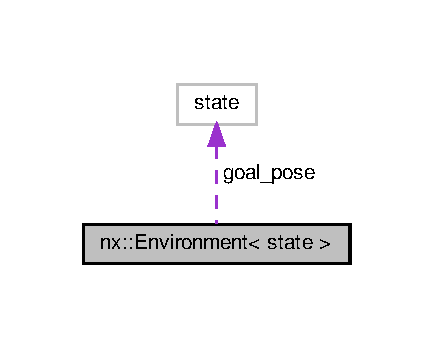
\includegraphics[width=208pt]{classnx_1_1Environment__coll__graph}
\end{center}
\end{figure}
\subsection*{Public Types}
\begin{DoxyCompactItemize}
\item 
\mbox{\Hypertarget{classnx_1_1Environment_a989675f3a115e396a169841ea96697c7}\label{classnx_1_1Environment_a989675f3a115e396a169841ea96697c7}} 
typedef \hyperlink{structnx_1_1MotionPrimitive}{Motion\+Primitive}$<$ std\+::array$<$ double, 3 $>$, std\+::array$<$ double, 2 $>$ $>$ {\bfseries M\+Prim}
\end{DoxyCompactItemize}
\subsection*{Public Member Functions}
\begin{DoxyCompactItemize}
\item 
\hyperlink{classnx_1_1Environment_a23652067c6e2c838b7e895ada850fa6b}{Environment} (std\+::shared\+\_\+ptr$<$ \hyperlink{classnx_1_1map__nd}{nx\+::map\+\_\+nd} $>$ map\+\_\+in, std\+::shared\+\_\+ptr$<$ std\+::vector$<$ char $>$$>$ cmap, state goal=state())
\item 
virtual void \hyperlink{classnx_1_1Environment_a5879e51878691196971e94880d45b551}{get\+\_\+succ} (const state \&curr, std\+::vector$<$ state $>$ \&succ, std\+::vector$<$ int $>$ \&succ\+\_\+idx, std\+::vector$<$ double $>$ \&succ\+\_\+cost, std\+::vector$<$ int $>$ \&action\+\_\+idx) const =0
\item 
virtual void \hyperlink{classnx_1_1Environment_a4f3ee5bb7665210e6262d333857e5f4f}{forward\+\_\+action} (const state \&curr, int action\+\_\+id, std\+::vector$<$ state $>$ \&next\+\_\+micro) const =0
\item 
virtual int \hyperlink{classnx_1_1Environment_a1c558036435de03a3afd85e940aad600}{state\+\_\+to\+\_\+idx} (const state \&) const =0
\item 
virtual std\+::vector$<$ int $>$ \hyperlink{classnx_1_1Environment_adb86237d799683c40f17c95ea39eeba3}{state\+\_\+to\+\_\+cell} (const state \&) const =0
\item 
virtual Vector3d \hyperlink{classnx_1_1Environment_ae31bd7f19efac45fc07d405f1fcfd2b2}{state\+\_\+to\+\_\+\+S\+E2} (const state \&) const =0
\item 
virtual double \hyperlink{classnx_1_1Environment_a25f01903609749dc40aa5ae07c0f5e06}{Compute\+State\+Metric} (const state \&, const state \&) const =0
\end{DoxyCompactItemize}
\subsection*{Public Attributes}
\begin{DoxyCompactItemize}
\item 
\mbox{\Hypertarget{classnx_1_1Environment_a5074fd389af065716dd7455e6eb58a10}\label{classnx_1_1Environment_a5074fd389af065716dd7455e6eb58a10}} 
std\+::shared\+\_\+ptr$<$ \hyperlink{classnx_1_1map__nd}{map\+\_\+nd} $>$ {\bfseries map}
\item 
\mbox{\Hypertarget{classnx_1_1Environment_a830b47524856d2074908a09883816a66}\label{classnx_1_1Environment_a830b47524856d2074908a09883816a66}} 
std\+::shared\+\_\+ptr$<$ std\+::vector$<$ char $>$ $>$ {\bfseries cmap\+\_\+}
\item 
\mbox{\Hypertarget{classnx_1_1Environment_a55d4d93f32e8259e2355f281ce290e02}\label{classnx_1_1Environment_a55d4d93f32e8259e2355f281ce290e02}} 
state {\bfseries goal\+\_\+pose}
\item 
\mbox{\Hypertarget{classnx_1_1Environment_af682fbcf24d8ec4ad43a80d0ccd64bba}\label{classnx_1_1Environment_af682fbcf24d8ec4ad43a80d0ccd64bba}} 
std\+::vector$<$ \hyperlink{structnx_1_1MotionPrimitive}{M\+Prim} $>$ {\bfseries mprim\+\_\+}
\end{DoxyCompactItemize}


\subsection{Constructor \& Destructor Documentation}
\mbox{\Hypertarget{classnx_1_1Environment_a23652067c6e2c838b7e895ada850fa6b}\label{classnx_1_1Environment_a23652067c6e2c838b7e895ada850fa6b}} 
\index{nx\+::\+Environment@{nx\+::\+Environment}!Environment@{Environment}}
\index{Environment@{Environment}!nx\+::\+Environment@{nx\+::\+Environment}}
\subsubsection{\texorpdfstring{Environment()}{Environment()}}
{\footnotesize\ttfamily template$<$class state$>$ \\
\hyperlink{classnx_1_1Environment}{nx\+::\+Environment}$<$ state $>$\+::\hyperlink{classnx_1_1Environment}{Environment} (\begin{DoxyParamCaption}\item[{std\+::shared\+\_\+ptr$<$ \hyperlink{classnx_1_1map__nd}{nx\+::map\+\_\+nd} $>$}]{map\+\_\+in,  }\item[{std\+::shared\+\_\+ptr$<$ std\+::vector$<$ char $>$$>$}]{cmap,  }\item[{state}]{goal = {\ttfamily state()} }\end{DoxyParamCaption})\hspace{0.3cm}{\ttfamily [inline]}}

Constructs an environment interface. 
\begin{DoxyParams}{Parameters}
{\em M\+A\+P\+\_\+ptr\+\_\+in} & The unique\+\_\+ptr to the map information. \\
\hline
{\em cmap} & The unique\+\_\+ptr to the cost\+Map. \\
\hline
{\em goal} & The optional goal coordinate. \\
\hline
\end{DoxyParams}


\subsection{Member Function Documentation}
\mbox{\Hypertarget{classnx_1_1Environment_a25f01903609749dc40aa5ae07c0f5e06}\label{classnx_1_1Environment_a25f01903609749dc40aa5ae07c0f5e06}} 
\index{nx\+::\+Environment@{nx\+::\+Environment}!Compute\+State\+Metric@{Compute\+State\+Metric}}
\index{Compute\+State\+Metric@{Compute\+State\+Metric}!nx\+::\+Environment@{nx\+::\+Environment}}
\subsubsection{\texorpdfstring{Compute\+State\+Metric()}{ComputeStateMetric()}}
{\footnotesize\ttfamily template$<$class state$>$ \\
virtual double \hyperlink{classnx_1_1Environment}{nx\+::\+Environment}$<$ state $>$\+::Compute\+State\+Metric (\begin{DoxyParamCaption}\item[{const state \&}]{,  }\item[{const state \&}]{ }\end{DoxyParamCaption}) const\hspace{0.3cm}{\ttfamily [pure virtual]}}

Computes the distance metric between two states. \begin{DoxyReturn}{Returns}
The distnace between the two states. 
\end{DoxyReturn}
\mbox{\Hypertarget{classnx_1_1Environment_a4f3ee5bb7665210e6262d333857e5f4f}\label{classnx_1_1Environment_a4f3ee5bb7665210e6262d333857e5f4f}} 
\index{nx\+::\+Environment@{nx\+::\+Environment}!forward\+\_\+action@{forward\+\_\+action}}
\index{forward\+\_\+action@{forward\+\_\+action}!nx\+::\+Environment@{nx\+::\+Environment}}
\subsubsection{\texorpdfstring{forward\+\_\+action()}{forward\_action()}}
{\footnotesize\ttfamily template$<$class state$>$ \\
virtual void \hyperlink{classnx_1_1Environment}{nx\+::\+Environment}$<$ state $>$\+::forward\+\_\+action (\begin{DoxyParamCaption}\item[{const state \&}]{curr,  }\item[{int}]{action\+\_\+id,  }\item[{std\+::vector$<$ state $>$ \&}]{next\+\_\+micro }\end{DoxyParamCaption}) const\hspace{0.3cm}{\ttfamily [pure virtual]}}

Computes the list of micro-\/states generated from applying the action with action\+\_\+id. 
\begin{DoxyParams}{Parameters}
{\em curr} & Current state. \\
\hline
{\em action\+\_\+id} & Action index to apply. \\
\hline
{\em next\+\_\+micro} & List of micro-\/states generated along the action. \\
\hline
\end{DoxyParams}


Implemented in \hyperlink{classnx_1_1SE2Environment_ac9453c2a57e53c9f511eb04aabaa0809}{nx\+::\+S\+E2\+Environment}.

\mbox{\Hypertarget{classnx_1_1Environment_a5879e51878691196971e94880d45b551}\label{classnx_1_1Environment_a5879e51878691196971e94880d45b551}} 
\index{nx\+::\+Environment@{nx\+::\+Environment}!get\+\_\+succ@{get\+\_\+succ}}
\index{get\+\_\+succ@{get\+\_\+succ}!nx\+::\+Environment@{nx\+::\+Environment}}
\subsubsection{\texorpdfstring{get\+\_\+succ()}{get\_succ()}}
{\footnotesize\ttfamily template$<$class state$>$ \\
virtual void \hyperlink{classnx_1_1Environment}{nx\+::\+Environment}$<$ state $>$\+::get\+\_\+succ (\begin{DoxyParamCaption}\item[{const state \&}]{curr,  }\item[{std\+::vector$<$ state $>$ \&}]{succ,  }\item[{std\+::vector$<$ int $>$ \&}]{succ\+\_\+idx,  }\item[{std\+::vector$<$ double $>$ \&}]{succ\+\_\+cost,  }\item[{std\+::vector$<$ int $>$ \&}]{action\+\_\+idx }\end{DoxyParamCaption}) const\hspace{0.3cm}{\ttfamily [pure virtual]}}

Computes the successor nodes from state curr, taking into account the cost\+Map. 
\begin{DoxyParams}{Parameters}
{\em curr} & The current state. \\
\hline
{\em succ} & The list of successors to be computed. \\
\hline
{\em succ\+\_\+idx} & The linear indices of the successors. \\
\hline
{\em succ\+\_\+cost} & \\
\hline
{\em action\+\_\+idx} & \\
\hline
\end{DoxyParams}


Implemented in \hyperlink{classnx_1_1SE2Environment_a2a4159dc6bf024e522bb504c77e9aa69}{nx\+::\+S\+E2\+Environment}.

\mbox{\Hypertarget{classnx_1_1Environment_adb86237d799683c40f17c95ea39eeba3}\label{classnx_1_1Environment_adb86237d799683c40f17c95ea39eeba3}} 
\index{nx\+::\+Environment@{nx\+::\+Environment}!state\+\_\+to\+\_\+cell@{state\+\_\+to\+\_\+cell}}
\index{state\+\_\+to\+\_\+cell@{state\+\_\+to\+\_\+cell}!nx\+::\+Environment@{nx\+::\+Environment}}
\subsubsection{\texorpdfstring{state\+\_\+to\+\_\+cell()}{state\_to\_cell()}}
{\footnotesize\ttfamily template$<$class state$>$ \\
virtual std\+::vector$<$int$>$ \hyperlink{classnx_1_1Environment}{nx\+::\+Environment}$<$ state $>$\+::state\+\_\+to\+\_\+cell (\begin{DoxyParamCaption}\item[{const state \&}]{ }\end{DoxyParamCaption}) const\hspace{0.3cm}{\ttfamily [pure virtual]}}

Converts a state to its corresponding cell coordinates in the map. \begin{DoxyReturn}{Returns}
The cell coordinates of the state. 
\end{DoxyReturn}


Implemented in \hyperlink{classnx_1_1SE2Environment_ae3ac780e46d421898e3c7db696d8026f}{nx\+::\+S\+E2\+Environment}.

\mbox{\Hypertarget{classnx_1_1Environment_a1c558036435de03a3afd85e940aad600}\label{classnx_1_1Environment_a1c558036435de03a3afd85e940aad600}} 
\index{nx\+::\+Environment@{nx\+::\+Environment}!state\+\_\+to\+\_\+idx@{state\+\_\+to\+\_\+idx}}
\index{state\+\_\+to\+\_\+idx@{state\+\_\+to\+\_\+idx}!nx\+::\+Environment@{nx\+::\+Environment}}
\subsubsection{\texorpdfstring{state\+\_\+to\+\_\+idx()}{state\_to\_idx()}}
{\footnotesize\ttfamily template$<$class state$>$ \\
virtual int \hyperlink{classnx_1_1Environment}{nx\+::\+Environment}$<$ state $>$\+::state\+\_\+to\+\_\+idx (\begin{DoxyParamCaption}\item[{const state \&}]{ }\end{DoxyParamCaption}) const\hspace{0.3cm}{\ttfamily [pure virtual]}}

Converts a state to its corresponding linear index in the map. \begin{DoxyReturn}{Returns}
The linear index of the state. 
\end{DoxyReturn}


Implemented in \hyperlink{classnx_1_1SE2Environment_a0fe7c5f438795a98f17be0ed95b2ff7c}{nx\+::\+S\+E2\+Environment}.

\mbox{\Hypertarget{classnx_1_1Environment_ae31bd7f19efac45fc07d405f1fcfd2b2}\label{classnx_1_1Environment_ae31bd7f19efac45fc07d405f1fcfd2b2}} 
\index{nx\+::\+Environment@{nx\+::\+Environment}!state\+\_\+to\+\_\+\+S\+E2@{state\+\_\+to\+\_\+\+S\+E2}}
\index{state\+\_\+to\+\_\+\+S\+E2@{state\+\_\+to\+\_\+\+S\+E2}!nx\+::\+Environment@{nx\+::\+Environment}}
\subsubsection{\texorpdfstring{state\+\_\+to\+\_\+\+S\+E2()}{state\_to\_SE2()}}
{\footnotesize\ttfamily template$<$class state$>$ \\
virtual Vector3d \hyperlink{classnx_1_1Environment}{nx\+::\+Environment}$<$ state $>$\+::state\+\_\+to\+\_\+\+S\+E2 (\begin{DoxyParamCaption}\item[{const state \&}]{ }\end{DoxyParamCaption}) const\hspace{0.3cm}{\ttfamily [pure virtual]}}

Returns the pose of the state, projecected into the S\+E(2) space, i.\+e. 2.\+5D position (X,Y,Yaw). \begin{DoxyReturn}{Returns}
The S\+E(2) Pose of the state. 
\end{DoxyReturn}


Implemented in \hyperlink{classnx_1_1SE2Environment_ab1f9056e6fffe905ec225ee3885679b4}{nx\+::\+S\+E2\+Environment}.



The documentation for this class was generated from the following file\+:\begin{DoxyCompactItemize}
\item 
include/igl/env/env\+\_\+int.\+h\end{DoxyCompactItemize}

\hypertarget{structnx_1_1GaussianBelief}{}\section{nx\+:\+:Gaussian\+Belief Struct Reference}
\label{structnx_1_1GaussianBelief}\index{nx\+::\+Gaussian\+Belief@{nx\+::\+Gaussian\+Belief}}


{\ttfamily \#include $<$kalman\+\_\+filter.\+h$>$}

\subsection*{Public Member Functions}
\begin{DoxyCompactItemize}
\item 
\hyperlink{structnx_1_1GaussianBelief_ab604fe9315b215ce1a6af633278d78ef}{Gaussian\+Belief} (const Vector\+Xd \&mean, const Matrix\+Xd \&covariance)
\end{DoxyCompactItemize}
\subsection*{Public Attributes}
\begin{DoxyCompactItemize}
\item 
\mbox{\Hypertarget{structnx_1_1GaussianBelief_a57b6672ced4ad92eca9f0dfb32391f67}\label{structnx_1_1GaussianBelief_a57b6672ced4ad92eca9f0dfb32391f67}} 
Vector\+Xd {\bfseries mean}
\item 
\mbox{\Hypertarget{structnx_1_1GaussianBelief_a4046d2db5369392801195631549fc658}\label{structnx_1_1GaussianBelief_a4046d2db5369392801195631549fc658}} 
Matrix\+Xd {\bfseries cov}
\end{DoxyCompactItemize}


\subsection{Detailed Description}
The \hyperlink{structnx_1_1GaussianBelief}{Gaussian\+Belief} struct stores a mean and covariance of a multivariate Gaussian distribution. 

\subsection{Constructor \& Destructor Documentation}
\mbox{\Hypertarget{structnx_1_1GaussianBelief_ab604fe9315b215ce1a6af633278d78ef}\label{structnx_1_1GaussianBelief_ab604fe9315b215ce1a6af633278d78ef}} 
\index{nx\+::\+Gaussian\+Belief@{nx\+::\+Gaussian\+Belief}!Gaussian\+Belief@{Gaussian\+Belief}}
\index{Gaussian\+Belief@{Gaussian\+Belief}!nx\+::\+Gaussian\+Belief@{nx\+::\+Gaussian\+Belief}}
\subsubsection{\texorpdfstring{Gaussian\+Belief()}{GaussianBelief()}}
{\footnotesize\ttfamily nx\+::\+Gaussian\+Belief\+::\+Gaussian\+Belief (\begin{DoxyParamCaption}\item[{const Vector\+Xd \&}]{mean,  }\item[{const Matrix\+Xd \&}]{covariance }\end{DoxyParamCaption})\hspace{0.3cm}{\ttfamily [inline]}}

Constructs the Gaussian Belief from a mean and covariance. 
\begin{DoxyParams}{Parameters}
{\em mean} & The mean of the Gaussian. \\
\hline
{\em covariance} & The covariance of the Gaussian. \\
\hline
\end{DoxyParams}


The documentation for this struct was generated from the following file\+:\begin{DoxyCompactItemize}
\item 
include/igl/estimation/kalman\+\_\+filter.\+h\end{DoxyCompactItemize}

\hypertarget{classnx_1_1InfoPlannerARVI}{}\section{nx\+:\+:Info\+Planner\+A\+R\+VI$<$ state $>$ Class Template Reference}
\label{classnx_1_1InfoPlannerARVI}\index{nx\+::\+Info\+Planner\+A\+R\+V\+I$<$ state $>$@{nx\+::\+Info\+Planner\+A\+R\+V\+I$<$ state $>$}}
\subsection*{Public Member Functions}
\begin{DoxyCompactItemize}
\item 
\hyperlink{classnx_1_1InfoPlannerARVI_abb908254580047ad273b6f9b9a8caf24}{Info\+Planner\+A\+R\+VI} (const int \&T, const double \&del=5, const double \&epsilon=std\+::numeric\+\_\+limits$<$ double $>$\+::infinity(), const double \&range=std\+::numeric\+\_\+limits$<$ double $>$\+::infinity(), const double \&allocated\+\_\+time\+\_\+secs=0.\+1, const int \&debug=0)
\item 
\mbox{\Hypertarget{classnx_1_1InfoPlannerARVI_a77fdbe59f157d0fef34118ad4655470e}\label{classnx_1_1InfoPlannerARVI_a77fdbe59f157d0fef34118ad4655470e}} 
\hyperlink{structnx_1_1PlannerOutput}{Planner\+Output}$<$ state $>$ {\bfseries Plan} (std\+::vector$<$ \hyperlink{classnx_1_1Robot}{nx\+::\+Robot}$<$ state $>$$>$ \&robots, int num, std\+::vector$<$ std\+::vector$<$ Vector\+Xd $>$$>$ fixed\+\_\+traj)
\item 
\mbox{\Hypertarget{classnx_1_1InfoPlannerARVI_a697b6b64459863124c7ef3f7daba7dc3}\label{classnx_1_1InfoPlannerARVI_a697b6b64459863124c7ef3f7daba7dc3}} 
\hyperlink{structnx_1_1PlannerOutput}{Planner\+Output}$<$ state $>$ {\bfseries PlanARVI\+Test} (std\+::vector$<$ \hyperlink{classnx_1_1Robot}{nx\+::\+Robot}$<$ state $>$$>$ \&robots, int num)
\end{DoxyCompactItemize}
\subsection*{Public Attributes}
\begin{DoxyCompactItemize}
\item 
\mbox{\Hypertarget{classnx_1_1InfoPlannerARVI_a471fe0c7b071380a34b309595441e1b6}\label{classnx_1_1InfoPlannerARVI_a471fe0c7b071380a34b309595441e1b6}} 
std\+::shared\+\_\+ptr$<$ \hyperlink{structnx_1_1InfoStateSpace}{Info\+State\+Space}$<$ state $>$ $>$ {\bfseries S\+\_\+t}
\end{DoxyCompactItemize}


\subsection{Constructor \& Destructor Documentation}
\mbox{\Hypertarget{classnx_1_1InfoPlannerARVI_abb908254580047ad273b6f9b9a8caf24}\label{classnx_1_1InfoPlannerARVI_abb908254580047ad273b6f9b9a8caf24}} 
\index{nx\+::\+Info\+Planner\+A\+R\+VI@{nx\+::\+Info\+Planner\+A\+R\+VI}!Info\+Planner\+A\+R\+VI@{Info\+Planner\+A\+R\+VI}}
\index{Info\+Planner\+A\+R\+VI@{Info\+Planner\+A\+R\+VI}!nx\+::\+Info\+Planner\+A\+R\+VI@{nx\+::\+Info\+Planner\+A\+R\+VI}}
\subsubsection{\texorpdfstring{Info\+Planner\+A\+R\+V\+I()}{InfoPlanner()}}
{\footnotesize\ttfamily template$<$class state $>$ \\
\hyperlink{classnx_1_1InfoPlannerARVI}{nx\+::\+Info\+Planner\+A\+R\+VI}$<$ state $>$\+::\hyperlink{classnx_1_1InfoPlannerARVI}{Info\+Planner\+A\+R\+VI} (\begin{DoxyParamCaption}\item[{const int \&}]{T,  }\item[{const double \&}]{del = {\ttfamily 5},  }\item[{const double \&}]{epsilon = {\ttfamily std\+:\+:numeric\+\_\+limits$<$double$>$\+:\+:infinity()},  }\item[{const double \&}]{range = {\ttfamily std\+:\+:numeric\+\_\+limits$<$double$>$\+:\+:infinity()},  }\item[{const double \&}]{allocated\+\_\+time\+\_\+secs = {\ttfamily 0.1},  }\item[{const int \&}]{debug = {\ttfamily 0} }\end{DoxyParamCaption})\hspace{0.3cm}{\ttfamily [inline]}}

Constructs an A\+R\+VI Planner. 
\begin{DoxyParams}{Parameters}
{\em T} & The planning horizon. \\
\hline
{\em del} & The initial value of delta. \\
\hline
{\em epsilon} & The initial value of epsilon. \\
\hline
{\em range} & Radius with which robots may plan jointly. \\
\hline
{\em allocated\+\_\+time\+\_\+secs} & Allocated A\+R\+VI Planning time. \\
\hline
{\em debug} & Whether the planner should print debug messages. \\
\hline
\end{DoxyParams}


The documentation for this class was generated from the following files\+:\begin{DoxyCompactItemize}
\item 
include/igl/planning/infoplanner\+\_\+arvi.\+h\item 
src/infoplanner\+\_\+arvi.\+cpp\end{DoxyCompactItemize}

\hypertarget{structnx_1_1InfoState}{}\section{nx\+:\+:Info\+State$<$ state $>$ Struct Template Reference}
\label{structnx_1_1InfoState}\index{nx\+::\+Info\+State$<$ state $>$@{nx\+::\+Info\+State$<$ state $>$}}
\subsection*{Public Member Functions}
\begin{DoxyCompactItemize}
\item 
\mbox{\Hypertarget{structnx_1_1InfoState_a582709ca7040dff17e5e2a9450bf171e}\label{structnx_1_1InfoState_a582709ca7040dff17e5e2a9450bf171e}} 
{\bfseries Info\+State} (int hashkey, const state \&coord, Matrix\+Xd \&Sigma, bool new\+\_\+state=false)
\end{DoxyCompactItemize}
\subsection*{Public Attributes}
\begin{DoxyCompactItemize}
\item 
\mbox{\Hypertarget{structnx_1_1InfoState_ac6e29a26329144f47969526f6a08a118}\label{structnx_1_1InfoState_ac6e29a26329144f47969526f6a08a118}} 
state {\bfseries coord}
\item 
\mbox{\Hypertarget{structnx_1_1InfoState_acbfbc2861af72e1ed79fbda6b7bed7b6}\label{structnx_1_1InfoState_acbfbc2861af72e1ed79fbda6b7bed7b6}} 
Matrix\+Xd {\bfseries Sigma}
\item 
\mbox{\Hypertarget{structnx_1_1InfoState_af5517b6744d3a95bb31bb3089da2b8ab}\label{structnx_1_1InfoState_af5517b6744d3a95bb31bb3089da2b8ab}} 
std\+::shared\+\_\+ptr$<$ \hyperlink{structnx_1_1InfoState}{Info\+State}$<$ state $>$ $>$ {\bfseries parent}
\item 
\mbox{\Hypertarget{structnx_1_1InfoState_a627fff266fc2bebc073e894edad47c59}\label{structnx_1_1InfoState_a627fff266fc2bebc073e894edad47c59}} 
int {\bfseries parent\+\_\+action\+\_\+id} = -\/1
\item 
\mbox{\Hypertarget{structnx_1_1InfoState_a4c7fb56d1594eab1df9dc522cee40dcb}\label{structnx_1_1InfoState_a4c7fb56d1594eab1df9dc522cee40dcb}} 
std\+::shared\+\_\+ptr$<$ cov\+Queue$<$ \hyperlink{structnx_1_1InfoState}{Info\+State}$<$ state $>$ $>$ $>$ {\bfseries state\+\_\+list}
\item 
\mbox{\Hypertarget{structnx_1_1InfoState_ad3cb2778af2b9ccd035d5ba81700fa83}\label{structnx_1_1InfoState_ad3cb2778af2b9ccd035d5ba81700fa83}} 
int {\bfseries hashkey}
\item 
\mbox{\Hypertarget{structnx_1_1InfoState_a4ef804a1e1e92344d8779d3d20b00ca0}\label{structnx_1_1InfoState_a4ef804a1e1e92344d8779d3d20b00ca0}} 
priority\+Queue$<$ \hyperlink{structnx_1_1InfoState}{Info\+State}$<$ state $>$ $>$\+::handle\+\_\+type {\bfseries heapkey}
\item 
\mbox{\Hypertarget{structnx_1_1InfoState_a625332147ae8ad23406ada2afec7ec7d}\label{structnx_1_1InfoState_a625332147ae8ad23406ada2afec7ec7d}} 
bool {\bfseries is\+\_\+open}
\item 
\mbox{\Hypertarget{structnx_1_1InfoState_a645cec83d8a2b212de7613a0835b2cca}\label{structnx_1_1InfoState_a645cec83d8a2b212de7613a0835b2cca}} 
bool {\bfseries is\+\_\+closed}
\item 
\mbox{\Hypertarget{structnx_1_1InfoState_aa2386d61df97eaa59d2d560f67b1cc5d}\label{structnx_1_1InfoState_aa2386d61df97eaa59d2d560f67b1cc5d}} 
double {\bfseries g} = std\+::numeric\+\_\+limits$<$double$>$\+::infinity()
\end{DoxyCompactItemize}


The documentation for this struct was generated from the following file\+:\begin{DoxyCompactItemize}
\item 
include/igl/planning/infoplanner\+\_\+arvi.\+h\end{DoxyCompactItemize}

\hypertarget{structnx_1_1InfoStateSpace}{}\section{nx\+:\+:Info\+State\+Space$<$ state $>$ Struct Template Reference}
\label{structnx_1_1InfoStateSpace}\index{nx\+::\+Info\+State\+Space$<$ state $>$@{nx\+::\+Info\+State\+Space$<$ state $>$}}
\subsection*{Public Attributes}
\begin{DoxyCompactItemize}
\item 
\mbox{\Hypertarget{structnx_1_1InfoStateSpace_a92784e02eccffbc05ecf76bdbe07a643}\label{structnx_1_1InfoStateSpace_a92784e02eccffbc05ecf76bdbe07a643}} 
priority\+Queue$<$ \hyperlink{structnx_1_1InfoState}{Info\+State}$<$ state $>$ $>$ {\bfseries pq}
\item 
\mbox{\Hypertarget{structnx_1_1InfoStateSpace_a24d71b39a47206a4d6da27154b12c9e0}\label{structnx_1_1InfoStateSpace_a24d71b39a47206a4d6da27154b12c9e0}} 
hash\+Map$<$ \hyperlink{structnx_1_1InfoState}{Info\+State}$<$ state $>$ $>$ {\bfseries hm}
\end{DoxyCompactItemize}


The documentation for this struct was generated from the following file\+:\begin{DoxyCompactItemize}
\item 
include/igl/planning/infoplanner\+\_\+arvi.\+h\end{DoxyCompactItemize}

\hypertarget{structnx_1_1InfoTarget}{}\section{nx\+:\+:Info\+Target Struct Reference}
\label{structnx_1_1InfoTarget}\index{nx\+::\+Info\+Target@{nx\+::\+Info\+Target}}


{\ttfamily \#include $<$info\+\_\+target\+\_\+model.\+h$>$}



Inheritance diagram for nx\+:\+:Info\+Target\+:
\nopagebreak
\begin{figure}[H]
\begin{center}
\leavevmode
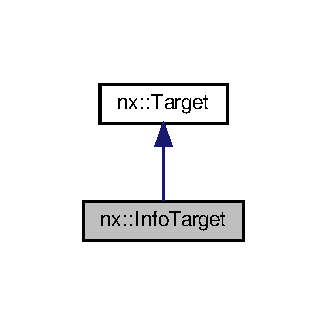
\includegraphics[width=157pt]{structnx_1_1InfoTarget__inherit__graph}
\end{center}
\end{figure}


Collaboration diagram for nx\+:\+:Info\+Target\+:
\nopagebreak
\begin{figure}[H]
\begin{center}
\leavevmode
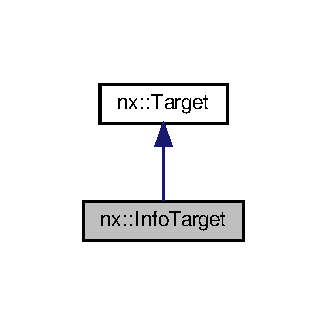
\includegraphics[width=157pt]{structnx_1_1InfoTarget__coll__graph}
\end{center}
\end{figure}
\subsection*{Public Member Functions}
\begin{DoxyCompactItemize}
\item 
\mbox{\Hypertarget{structnx_1_1InfoTarget_a00952ad1d04afb571a3f5c71447f7bb3}\label{structnx_1_1InfoTarget_a00952ad1d04afb571a3f5c71447f7bb3}} 
{\bfseries Info\+Target} (int ID, const Vector\+Xd \&state, const Matrix\+Xd \&A, const Matrix\+Xd \&W, const Matrix\+Xd \&covariance)
\item 
\mbox{\Hypertarget{structnx_1_1InfoTarget_a169b44c7fdef239d040b1438ee881b48}\label{structnx_1_1InfoTarget_a169b44c7fdef239d040b1438ee881b48}} 
void {\bfseries Update\+Belief} (Vector\+Xd mean, Matrix\+Xd cov)
\end{DoxyCompactItemize}
\subsection*{Public Attributes}
\begin{DoxyCompactItemize}
\item 
\mbox{\Hypertarget{structnx_1_1InfoTarget_a74fe130d7cc4f682e7f0d8bab46a8440}\label{structnx_1_1InfoTarget_a74fe130d7cc4f682e7f0d8bab46a8440}} 
Matrix\+Xd {\bfseries covariance}
\end{DoxyCompactItemize}


\subsection{Detailed Description}
The \hyperlink{structnx_1_1InfoTarget}{Info\+Target} class extends the \hyperlink{structnx_1_1Target}{Target} class to include a covariance matrix, so that it supports a gaussian probability distribution over targets. 

The documentation for this struct was generated from the following file\+:\begin{DoxyCompactItemize}
\item 
include/igl/target\+\_\+motion\+\_\+models/info\+\_\+target\+\_\+model.\+h\end{DoxyCompactItemize}

\hypertarget{classnx_1_1InfoTargetModel}{}\section{nx\+:\+:Info\+Target\+Model Class Reference}
\label{classnx_1_1InfoTargetModel}\index{nx\+::\+Info\+Target\+Model@{nx\+::\+Info\+Target\+Model}}


{\ttfamily \#include $<$info\+\_\+target\+\_\+model.\+h$>$}



Inheritance diagram for nx\+:\+:Info\+Target\+Model\+:
\nopagebreak
\begin{figure}[H]
\begin{center}
\leavevmode
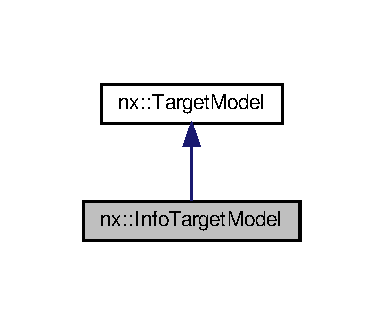
\includegraphics[width=184pt]{classnx_1_1InfoTargetModel__inherit__graph}
\end{center}
\end{figure}


Collaboration diagram for nx\+:\+:Info\+Target\+Model\+:
\nopagebreak
\begin{figure}[H]
\begin{center}
\leavevmode
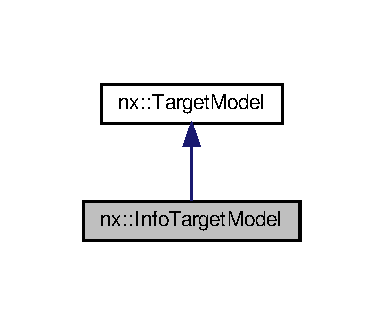
\includegraphics[width=184pt]{classnx_1_1InfoTargetModel__coll__graph}
\end{center}
\end{figure}
\subsection*{Public Member Functions}
\begin{DoxyCompactItemize}
\item 
\hyperlink{classnx_1_1InfoTargetModel_a23f4a00fd334292a91af451f2278310d}{Info\+Target\+Model} ()
\item 
\mbox{\Hypertarget{classnx_1_1InfoTargetModel_add9b3da880f99e8a0eb8a28921792bfa}\label{classnx_1_1InfoTargetModel_add9b3da880f99e8a0eb8a28921792bfa}} 
bool {\bfseries Add\+Target} (int ID, const \hyperlink{structnx_1_1InfoTarget}{Info\+Target} \&target)
\item 
Matrix\+Xd \hyperlink{classnx_1_1InfoTargetModel_a9387b0bd4e3e6d59570be7e7b369f792}{Get\+Covariance\+Matrix} () const
\item 
void \hyperlink{classnx_1_1InfoTargetModel_ab5c829223d48549889ef74d10bb8c408}{Update\+Belief} (Vector\+Xd mean, Matrix\+Xd covariance)
\item 
void \hyperlink{classnx_1_1InfoTargetModel_a371e2e95065f12fb672063eef87fa8c7}{Get\+Jacobian} (Matrix\+Xd \&A\+\_\+, Matrix\+Xd \&W\+\_\+) const
\item 
std\+::shared\+\_\+ptr$<$ \hyperlink{structnx_1_1InfoTarget}{Info\+Target} $>$ \hyperlink{classnx_1_1InfoTargetModel_add48b716a418b07c386cbe4726671540}{Get\+Target\+By\+ID} (int ID) const
\end{DoxyCompactItemize}
\subsection*{Additional Inherited Members}


\subsection{Detailed Description}
The info\+Target\+Model class extends target\+Model in order to maintain a Gaussian distribution over the target state (mean, and covariance). This is useful for a robot\textquotesingle{}s internal representation of the target. 

\subsection{Constructor \& Destructor Documentation}
\mbox{\Hypertarget{classnx_1_1InfoTargetModel_a23f4a00fd334292a91af451f2278310d}\label{classnx_1_1InfoTargetModel_a23f4a00fd334292a91af451f2278310d}} 
\index{nx\+::\+Info\+Target\+Model@{nx\+::\+Info\+Target\+Model}!Info\+Target\+Model@{Info\+Target\+Model}}
\index{Info\+Target\+Model@{Info\+Target\+Model}!nx\+::\+Info\+Target\+Model@{nx\+::\+Info\+Target\+Model}}
\subsubsection{\texorpdfstring{Info\+Target\+Model()}{InfoTargetModel()}}
{\footnotesize\ttfamily nx\+::\+Info\+Target\+Model\+::\+Info\+Target\+Model (\begin{DoxyParamCaption}{ }\end{DoxyParamCaption})\hspace{0.3cm}{\ttfamily [inline]}}

Default Constructor. 

\subsection{Member Function Documentation}
\mbox{\Hypertarget{classnx_1_1InfoTargetModel_a9387b0bd4e3e6d59570be7e7b369f792}\label{classnx_1_1InfoTargetModel_a9387b0bd4e3e6d59570be7e7b369f792}} 
\index{nx\+::\+Info\+Target\+Model@{nx\+::\+Info\+Target\+Model}!Get\+Covariance\+Matrix@{Get\+Covariance\+Matrix}}
\index{Get\+Covariance\+Matrix@{Get\+Covariance\+Matrix}!nx\+::\+Info\+Target\+Model@{nx\+::\+Info\+Target\+Model}}
\subsubsection{\texorpdfstring{Get\+Covariance\+Matrix()}{GetCovarianceMatrix()}}
{\footnotesize\ttfamily Matrix\+Xd nx\+::\+Info\+Target\+Model\+::\+Get\+Covariance\+Matrix (\begin{DoxyParamCaption}{ }\end{DoxyParamCaption}) const\hspace{0.3cm}{\ttfamily [inline]}}

Returns the joint system matrix A of the target model. \begin{DoxyReturn}{Returns}
The system matrix. 
\end{DoxyReturn}
\mbox{\Hypertarget{classnx_1_1InfoTargetModel_a371e2e95065f12fb672063eef87fa8c7}\label{classnx_1_1InfoTargetModel_a371e2e95065f12fb672063eef87fa8c7}} 
\index{nx\+::\+Info\+Target\+Model@{nx\+::\+Info\+Target\+Model}!Get\+Jacobian@{Get\+Jacobian}}
\index{Get\+Jacobian@{Get\+Jacobian}!nx\+::\+Info\+Target\+Model@{nx\+::\+Info\+Target\+Model}}
\subsubsection{\texorpdfstring{Get\+Jacobian()}{GetJacobian()}}
{\footnotesize\ttfamily void nx\+::\+Info\+Target\+Model\+::\+Get\+Jacobian (\begin{DoxyParamCaption}\item[{Matrix\+Xd \&}]{A\+\_\+,  }\item[{Matrix\+Xd \&}]{W\+\_\+ }\end{DoxyParamCaption}) const\hspace{0.3cm}{\ttfamily [inline]}}

Assigns the Jacobian for the \hyperlink{structnx_1_1Target}{Target} motion model. 
\begin{DoxyParams}{Parameters}
{\em A\+\_\+} & \\
\hline
{\em W\+\_\+} & \\
\hline
\end{DoxyParams}
\mbox{\Hypertarget{classnx_1_1InfoTargetModel_add48b716a418b07c386cbe4726671540}\label{classnx_1_1InfoTargetModel_add48b716a418b07c386cbe4726671540}} 
\index{nx\+::\+Info\+Target\+Model@{nx\+::\+Info\+Target\+Model}!Get\+Target\+By\+ID@{Get\+Target\+By\+ID}}
\index{Get\+Target\+By\+ID@{Get\+Target\+By\+ID}!nx\+::\+Info\+Target\+Model@{nx\+::\+Info\+Target\+Model}}
\subsubsection{\texorpdfstring{Get\+Target\+By\+I\+D()}{GetTargetByID()}}
{\footnotesize\ttfamily std\+::shared\+\_\+ptr$<$\hyperlink{structnx_1_1InfoTarget}{Info\+Target}$>$ nx\+::\+Info\+Target\+Model\+::\+Get\+Target\+By\+ID (\begin{DoxyParamCaption}\item[{int}]{ID }\end{DoxyParamCaption}) const\hspace{0.3cm}{\ttfamily [inline]}}

Returns the \hyperlink{structnx_1_1InfoTarget}{Info\+Target} by ID 
\begin{DoxyParams}{Parameters}
{\em ID} & The ID of the target to return. \\
\hline
\end{DoxyParams}
\begin{DoxyReturn}{Returns}
The \hyperlink{structnx_1_1InfoTarget}{Info\+Target} queried for. 
\end{DoxyReturn}
\mbox{\Hypertarget{classnx_1_1InfoTargetModel_ab5c829223d48549889ef74d10bb8c408}\label{classnx_1_1InfoTargetModel_ab5c829223d48549889ef74d10bb8c408}} 
\index{nx\+::\+Info\+Target\+Model@{nx\+::\+Info\+Target\+Model}!Update\+Belief@{Update\+Belief}}
\index{Update\+Belief@{Update\+Belief}!nx\+::\+Info\+Target\+Model@{nx\+::\+Info\+Target\+Model}}
\subsubsection{\texorpdfstring{Update\+Belief()}{UpdateBelief()}}
{\footnotesize\ttfamily void nx\+::\+Info\+Target\+Model\+::\+Update\+Belief (\begin{DoxyParamCaption}\item[{Vector\+Xd}]{mean,  }\item[{Matrix\+Xd}]{covariance }\end{DoxyParamCaption})\hspace{0.3cm}{\ttfamily [inline]}}

Updates the Information State of the \hyperlink{structnx_1_1Target}{Target} Model. 
\begin{DoxyParams}{Parameters}
{\em y\+\_\+} & The new mean. \\
\hline
{\em Sigma\+\_\+} & The new covariance. \\
\hline
\end{DoxyParams}


The documentation for this class was generated from the following file\+:\begin{DoxyCompactItemize}
\item 
include/igl/target\+\_\+motion\+\_\+models/info\+\_\+target\+\_\+model.\+h\end{DoxyCompactItemize}

\hypertarget{classnx_1_1SE3Pose_1_1InvalidOrientation}{}\section{nx\+:\+:S\+E3\+Pose\+:\+:Invalid\+Orientation Class Reference}
\label{classnx_1_1SE3Pose_1_1InvalidOrientation}\index{nx\+::\+S\+E3\+Pose\+::\+Invalid\+Orientation@{nx\+::\+S\+E3\+Pose\+::\+Invalid\+Orientation}}


{\ttfamily \#include $<$se3\+\_\+pose.\+h$>$}



Inheritance diagram for nx\+:\+:S\+E3\+Pose\+:\+:Invalid\+Orientation\+:
\nopagebreak
\begin{figure}[H]
\begin{center}
\leavevmode
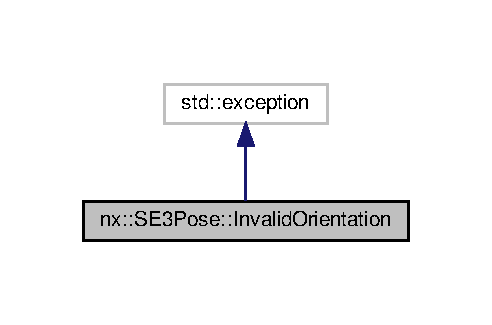
\includegraphics[width=236pt]{classnx_1_1SE3Pose_1_1InvalidOrientation__inherit__graph}
\end{center}
\end{figure}


Collaboration diagram for nx\+:\+:S\+E3\+Pose\+:\+:Invalid\+Orientation\+:
\nopagebreak
\begin{figure}[H]
\begin{center}
\leavevmode
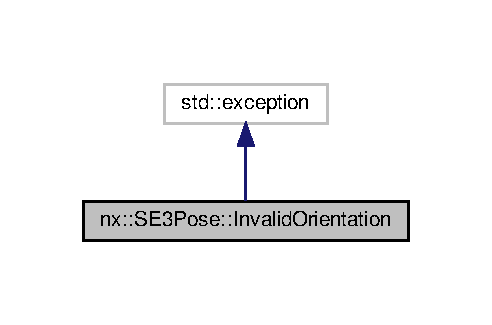
\includegraphics[width=236pt]{classnx_1_1SE3Pose_1_1InvalidOrientation__coll__graph}
\end{center}
\end{figure}


\subsection{Detailed Description}
Exception to throw if an invalid orientation is given. 

The documentation for this class was generated from the following file\+:\begin{DoxyCompactItemize}
\item 
include/igl/se3\+\_\+pose.\+h\end{DoxyCompactItemize}

\hypertarget{classnx_1_1KalmanFilter}{}\section{nx\+:\+:Kalman\+Filter Class Reference}
\label{classnx_1_1KalmanFilter}\index{nx\+::\+Kalman\+Filter@{nx\+::\+Kalman\+Filter}}


{\ttfamily \#include $<$kalman\+\_\+filter.\+h$>$}

\subsection*{Static Public Member Functions}
\begin{DoxyCompactItemize}
\item 
static Matrix\+Xd \hyperlink{classnx_1_1KalmanFilter_a1335cc928085a2c01b6a6a0d56e36903}{K\+F\+Covariance} (const Matrix\+Xd \&cov\+\_\+prior, const Matrix\+Xd \&A, const Matrix\+Xd \&W, const Matrix\+Xd \&H, const Matrix\+Xd \&V)
\item 
static \hyperlink{structnx_1_1GaussianBelief}{Gaussian\+Belief} \hyperlink{classnx_1_1KalmanFilter_a3c58332273552a6ea9133c54f3f74986}{KF} (const Vector\+Xd \&innovation, const Vector\+Xd \&mean\+\_\+prior, const Matrix\+Xd \&cov\+\_\+prior, const Matrix\+Xd \&A, const Matrix\+Xd \&W, const Matrix\+Xd \&H, const Matrix\+Xd \&V, int debug=0)
\end{DoxyCompactItemize}


\subsection{Detailed Description}
The \hyperlink{classnx_1_1KalmanFilter}{Kalman\+Filter} class contains static methods which execute the predict and update steps of a Kalman Filter, both with and without measurements. 

\subsection{Member Function Documentation}
\mbox{\Hypertarget{classnx_1_1KalmanFilter_a3c58332273552a6ea9133c54f3f74986}\label{classnx_1_1KalmanFilter_a3c58332273552a6ea9133c54f3f74986}} 
\index{nx\+::\+Kalman\+Filter@{nx\+::\+Kalman\+Filter}!KF@{KF}}
\index{KF@{KF}!nx\+::\+Kalman\+Filter@{nx\+::\+Kalman\+Filter}}
\subsubsection{\texorpdfstring{K\+F()}{KF()}}
{\footnotesize\ttfamily static \hyperlink{structnx_1_1GaussianBelief}{Gaussian\+Belief} nx\+::\+Kalman\+Filter\+::\+KF (\begin{DoxyParamCaption}\item[{const Vector\+Xd \&}]{innovation,  }\item[{const Vector\+Xd \&}]{mean\+\_\+prior,  }\item[{const Matrix\+Xd \&}]{cov\+\_\+prior,  }\item[{const Matrix\+Xd \&}]{A,  }\item[{const Matrix\+Xd \&}]{W,  }\item[{const Matrix\+Xd \&}]{H,  }\item[{const Matrix\+Xd \&}]{V,  }\item[{int}]{debug = {\ttfamily 0} }\end{DoxyParamCaption})\hspace{0.3cm}{\ttfamily [inline]}, {\ttfamily [static]}}

The KF function takes as input the innovation vector, and prior Gaussian distribution to compute the Kalman Filter prediction and update steps to compute a posterior Gaussian distribution. 
\begin{DoxyParams}{Parameters}
{\em innovation} & The innovation vector, i.\+e. z -\/ h(mean). \\
\hline
{\em mean\+\_\+prior} & The prior mean. \\
\hline
{\em cov\+\_\+prior} & The prior covariance matrix. \\
\hline
{\em A} & The system dynamics matrix. \\
\hline
{\em W} & The system noise matrix. \\
\hline
{\em H} & The observation model matrix. \\
\hline
{\em V} & The observation model noise matrix. \\
\hline
\end{DoxyParams}
\begin{DoxyReturn}{Returns}
The posterior Gaussian belief. 
\end{DoxyReturn}
\mbox{\Hypertarget{classnx_1_1KalmanFilter_a1335cc928085a2c01b6a6a0d56e36903}\label{classnx_1_1KalmanFilter_a1335cc928085a2c01b6a6a0d56e36903}} 
\index{nx\+::\+Kalman\+Filter@{nx\+::\+Kalman\+Filter}!K\+F\+Covariance@{K\+F\+Covariance}}
\index{K\+F\+Covariance@{K\+F\+Covariance}!nx\+::\+Kalman\+Filter@{nx\+::\+Kalman\+Filter}}
\subsubsection{\texorpdfstring{K\+F\+Covariance()}{KFCovariance()}}
{\footnotesize\ttfamily static Matrix\+Xd nx\+::\+Kalman\+Filter\+::\+K\+F\+Covariance (\begin{DoxyParamCaption}\item[{const Matrix\+Xd \&}]{cov\+\_\+prior,  }\item[{const Matrix\+Xd \&}]{A,  }\item[{const Matrix\+Xd \&}]{W,  }\item[{const Matrix\+Xd \&}]{H,  }\item[{const Matrix\+Xd \&}]{V }\end{DoxyParamCaption})\hspace{0.3cm}{\ttfamily [inline]}, {\ttfamily [static]}}

The K\+F\+Covariance function takes as input a prior covariance matrix, and computes the Kalman filter prediction and update steps to calculate the posterior covariance matrix. Note that the covariance posterior is deterministic and does not depend on the measurement values. 
\begin{DoxyParams}{Parameters}
{\em cov\+\_\+prior} & The prior covariance matrix. \\
\hline
{\em A} & The system dynamics matrix. \\
\hline
{\em W} & The system noise matrix. \\
\hline
{\em H} & The observation model matrix. \\
\hline
{\em V} & The observation model noise matrix. \\
\hline
\end{DoxyParams}
\begin{DoxyReturn}{Returns}
The posterior covariance matrix. 
\end{DoxyReturn}


The documentation for this class was generated from the following file\+:\begin{DoxyCompactItemize}
\item 
include/igl/estimation/kalman\+\_\+filter.\+h\end{DoxyCompactItemize}

\hypertarget{classnx_1_1Logger}{}\section{nx\+:\+:Logger Class Reference}
\label{classnx_1_1Logger}\index{nx\+::\+Logger@{nx\+::\+Logger}}
\subsection*{Public Member Functions}
\begin{DoxyCompactItemize}
\item 
\mbox{\Hypertarget{classnx_1_1Logger_a639bf5ba9ecd1ead5cc27ff67af557e8}\label{classnx_1_1Logger_a639bf5ba9ecd1ead5cc27ff67af557e8}} 
{\bfseries Logger} (int n\+\_\+robots, int n\+\_\+targets, int target\+\_\+dim, int Tmax)
\item 
\mbox{\Hypertarget{classnx_1_1Logger_a8ab63781a718f2866798fae568b226d1}\label{classnx_1_1Logger_a8ab63781a718f2866798fae568b226d1}} 
void {\bfseries Log\+Data} ()
\item 
\mbox{\Hypertarget{classnx_1_1Logger_ac85aeb9fb5a7dac9dc498403b4b9d4ca}\label{classnx_1_1Logger_ac85aeb9fb5a7dac9dc498403b4b9d4ca}} 
void {\bfseries write\+Data} ()
\end{DoxyCompactItemize}
\subsection*{Public Attributes}
\begin{DoxyCompactItemize}
\item 
\mbox{\Hypertarget{classnx_1_1Logger_aa3506a88a672d3bc6eb9473b52622948}\label{classnx_1_1Logger_aa3506a88a672d3bc6eb9473b52622948}} 
int {\bfseries max\+\_\+targets} = 0
\item 
\mbox{\Hypertarget{classnx_1_1Logger_ac65b9e29fd03448e942a583d71166b1a}\label{classnx_1_1Logger_ac65b9e29fd03448e942a583d71166b1a}} 
std\+::vector$<$ std\+::list$<$ Vector\+Xd $>$ $>$ {\bfseries y\+\_\+est\+\_\+list}
\item 
\mbox{\Hypertarget{classnx_1_1Logger_a000119f552228bdf07c7550e4bb2b4c2}\label{classnx_1_1Logger_a000119f552228bdf07c7550e4bb2b4c2}} 
std\+::vector$<$ std\+::list$<$ Matrix\+Xd $>$ $>$ {\bfseries Sigma\+\_\+est\+\_\+list}
\item 
\mbox{\Hypertarget{classnx_1_1Logger_a51f038ccd6570dce012eddb6bfe056db}\label{classnx_1_1Logger_a51f038ccd6570dce012eddb6bfe056db}} 
std\+::vector$<$ std\+::list$<$ std\+::map$<$ int, int $>$ $>$ $>$ {\bfseries da\+\_\+i}
\item 
\mbox{\Hypertarget{classnx_1_1Logger_ab2b15aed42a57becc31f4ee5151abf68}\label{classnx_1_1Logger_ab2b15aed42a57becc31f4ee5151abf68}} 
std\+::vector$<$ std\+::list$<$ std\+::map$<$ int, int $>$ $>$ $>$ {\bfseries da\+\_\+ir}
\item 
\mbox{\Hypertarget{classnx_1_1Logger_a0b60cc34934f4e18ef6836c0ffa29bcb}\label{classnx_1_1Logger_a0b60cc34934f4e18ef6836c0ffa29bcb}} 
Matrix\+Xd {\bfseries Ground\+\_\+truth}
\item 
\mbox{\Hypertarget{classnx_1_1Logger_ad983be62737edf231f65219838817c9b}\label{classnx_1_1Logger_ad983be62737edf231f65219838817c9b}} 
Matrix\+Xd {\bfseries Ground\+\_\+truth\+\_\+da}
\item 
\mbox{\Hypertarget{classnx_1_1Logger_aa83de5593f43e114f58a618e34b5398c}\label{classnx_1_1Logger_aa83de5593f43e114f58a618e34b5398c}} 
Matrix\+Xd {\bfseries robot\+\_\+pos}
\item 
\mbox{\Hypertarget{classnx_1_1Logger_a2c0d91651c288f69d44d8cc825faedf8}\label{classnx_1_1Logger_a2c0d91651c288f69d44d8cc825faedf8}} 
int {\bfseries n\+\_\+robots}
\item 
\mbox{\Hypertarget{classnx_1_1Logger_a51a5845a83ea3018ce7e9a4f4d127f7f}\label{classnx_1_1Logger_a51a5845a83ea3018ce7e9a4f4d127f7f}} 
int {\bfseries Tmax}
\end{DoxyCompactItemize}


The documentation for this class was generated from the following file\+:\begin{DoxyCompactItemize}
\item 
include/igl/utils/logger.\+h\end{DoxyCompactItemize}

\hypertarget{classnx_1_1map__nd}{}\section{nx\+:\+:map\+\_\+nd Class Reference}
\label{classnx_1_1map__nd}\index{nx\+::map\+\_\+nd@{nx\+::map\+\_\+nd}}
\subsection*{Public Member Functions}
\begin{DoxyCompactItemize}
\item 
\mbox{\Hypertarget{classnx_1_1map__nd_a78f5e0bfb0c62de795de24fa81ce9bdd}\label{classnx_1_1map__nd_a78f5e0bfb0c62de795de24fa81ce9bdd}} 
{\bfseries map\+\_\+nd} (std\+::vector$<$ double $>$ const \&devmin, std\+::vector$<$ double $>$ const \&devmax, std\+::vector$<$ double $>$ const \&resolution)
\item 
\mbox{\Hypertarget{classnx_1_1map__nd_aebac1dd3f2bab505be8374ffd61ec00d}\label{classnx_1_1map__nd_aebac1dd3f2bab505be8374ffd61ec00d}} 
{\bfseries map\+\_\+nd} (std\+::vector$<$ double $>$ const \&devmin, std\+::vector$<$ double $>$ const \&devmax, double resolution)
\item 
\mbox{\Hypertarget{classnx_1_1map__nd_a7d0ac18594ca1e05616455426f8cdca5}\label{classnx_1_1map__nd_a7d0ac18594ca1e05616455426f8cdca5}} 
{\bfseries map\+\_\+nd} (size\+\_\+t num\+\_\+dim, double $\ast$devmin, double $\ast$devmax, double $\ast$resolution)
\item 
\mbox{\Hypertarget{classnx_1_1map__nd_a81362efe2df41defa05895a5f0be544f}\label{classnx_1_1map__nd_a81362efe2df41defa05895a5f0be544f}} 
{\bfseries map\+\_\+nd} (size\+\_\+t num\+\_\+dim, double $\ast$devmin, double $\ast$devmax, double resolution)
\item 
\mbox{\Hypertarget{classnx_1_1map__nd_a7b6ca0645b4632fe932caed1decf0787}\label{classnx_1_1map__nd_a7b6ca0645b4632fe932caed1decf0787}} 
{\bfseries map\+\_\+nd} (const std\+::vector$<$ int $>$ \&oddsize, const std\+::vector$<$ double $>$ \&origin, const std\+::vector$<$ double $>$ \&resolution)
\item 
\mbox{\Hypertarget{classnx_1_1map__nd_a6e54390d4b7d58686e43b5b4c260c800}\label{classnx_1_1map__nd_a6e54390d4b7d58686e43b5b4c260c800}} 
std\+::vector$<$ double $>$ const  \& {\bfseries min} (void) const
\item 
\mbox{\Hypertarget{classnx_1_1map__nd_aff7c7163aebf20b3422f69961ed31323}\label{classnx_1_1map__nd_aff7c7163aebf20b3422f69961ed31323}} 
std\+::vector$<$ double $>$ const  \& {\bfseries max} (void) const
\item 
\mbox{\Hypertarget{classnx_1_1map__nd_a57c82d390b1d270e45014e65d909192e}\label{classnx_1_1map__nd_a57c82d390b1d270e45014e65d909192e}} 
std\+::vector$<$ double $>$ const  \& {\bfseries res} (void) const
\item 
\mbox{\Hypertarget{classnx_1_1map__nd_afd46d0ec66c4ddf6261441307c15e5f4}\label{classnx_1_1map__nd_afd46d0ec66c4ddf6261441307c15e5f4}} 
std\+::vector$<$ int $>$ const  \& {\bfseries size} (void) const
\item 
\mbox{\Hypertarget{classnx_1_1map__nd_a42a539afe36fafeba5ff9ee763cf3037}\label{classnx_1_1map__nd_a42a539afe36fafeba5ff9ee763cf3037}} 
std\+::vector$<$ double $>$ const  \& {\bfseries origin} (void) const
\item 
\mbox{\Hypertarget{classnx_1_1map__nd_ab4fada7238c9ead0429f6d6d0dc371f1}\label{classnx_1_1map__nd_ab4fada7238c9ead0429f6d6d0dc371f1}} 
std\+::vector$<$ int $>$ const  \& {\bfseries origincells} (void) const
\item 
\mbox{\Hypertarget{classnx_1_1map__nd_a0d2f2778ab2d91f0840f5a9b786a4447}\label{classnx_1_1map__nd_a0d2f2778ab2d91f0840f5a9b786a4447}} 
std\+::vector$<$ int $>$ {\bfseries meters2cells} (const std\+::vector$<$ double $>$ \&datam) const
\item 
\mbox{\Hypertarget{classnx_1_1map__nd_ad1d6b6df4e260605631d87401f037fe9}\label{classnx_1_1map__nd_ad1d6b6df4e260605631d87401f037fe9}} 
std\+::vector$<$ double $>$ {\bfseries cells2meters} (const std\+::vector$<$ int $>$ \&datac) const
\item 
\mbox{\Hypertarget{classnx_1_1map__nd_a62843a8aac41a26ac9012c52679495a1}\label{classnx_1_1map__nd_a62843a8aac41a26ac9012c52679495a1}} 
std\+::vector$<$ double $>$ {\bfseries meters2cells\+\_\+cont} (const std\+::vector$<$ double $>$ \&datam) const
\item 
\mbox{\Hypertarget{classnx_1_1map__nd_ab244a7b794c91e1353d89635350eff4f}\label{classnx_1_1map__nd_ab244a7b794c91e1353d89635350eff4f}} 
std\+::vector$<$ int $>$ {\bfseries meters2cells} (const std\+::vector$<$ double $>$\+::const\+\_\+iterator \&datam\+\_\+begin, const std\+::vector$<$ double $>$\+::const\+\_\+iterator \&datam\+\_\+end) const
\item 
\mbox{\Hypertarget{classnx_1_1map__nd_a8dd3781d0adca6adc7c84ea3725b06ca}\label{classnx_1_1map__nd_a8dd3781d0adca6adc7c84ea3725b06ca}} 
std\+::vector$<$ double $>$ {\bfseries cells2meters} (const std\+::vector$<$ int $>$\+::const\+\_\+iterator \&datac\+\_\+begin, const std\+::vector$<$ int $>$\+::const\+\_\+iterator \&datac\+\_\+end) const
\item 
\mbox{\Hypertarget{classnx_1_1map__nd_a4d3ecbe0fcd2927e38e4cf016a614547}\label{classnx_1_1map__nd_a4d3ecbe0fcd2927e38e4cf016a614547}} 
std\+::vector$<$ double $>$ {\bfseries meters2cells\+\_\+cont} (const std\+::vector$<$ double $>$\+::const\+\_\+iterator \&datam\+\_\+begin, const std\+::vector$<$ double $>$\+::const\+\_\+iterator \&datam\+\_\+end) const
\item 
\mbox{\Hypertarget{classnx_1_1map__nd_aa37889a8c513a7d56394e62f31419dea}\label{classnx_1_1map__nd_aa37889a8c513a7d56394e62f31419dea}} 
int {\bfseries subv2ind\+\_\+rowmajor} (std\+::vector$<$ int $>$ const \&datac) const
\item 
\mbox{\Hypertarget{classnx_1_1map__nd_afe4a818dd9e09c399977518ca6ed601c}\label{classnx_1_1map__nd_afe4a818dd9e09c399977518ca6ed601c}} 
std\+::vector$<$ int $>$ {\bfseries ind2subv\+\_\+rowmajor} (int ind) const
\item 
\mbox{\Hypertarget{classnx_1_1map__nd_a7fb171f334cc7bae6c5460a95dfe77f2}\label{classnx_1_1map__nd_a7fb171f334cc7bae6c5460a95dfe77f2}} 
int {\bfseries subv2ind\+\_\+colmajor} (std\+::vector$<$ int $>$ const \&datac) const
\item 
\mbox{\Hypertarget{classnx_1_1map__nd_a1c26f34a257da1a383c44fc395da026f}\label{classnx_1_1map__nd_a1c26f34a257da1a383c44fc395da026f}} 
std\+::vector$<$ int $>$ {\bfseries ind2subv\+\_\+colmajor} (int ind) const
\item 
\mbox{\Hypertarget{classnx_1_1map__nd_ad92e02c6e22712e221669ecef801ddc6}\label{classnx_1_1map__nd_ad92e02c6e22712e221669ecef801ddc6}} 
{\footnotesize template$<$class T $>$ }\\std\+::vector$<$ T $>$ {\bfseries rowmajor2colmajor} (const std\+::vector$<$ T $>$ \&map) const
\item 
\mbox{\Hypertarget{classnx_1_1map__nd_ad59bef0b0ad7233cf712ab9feab536f1}\label{classnx_1_1map__nd_ad59bef0b0ad7233cf712ab9feab536f1}} 
{\footnotesize template$<$class T $>$ }\\std\+::vector$<$ T $>$ {\bfseries colmajor2rowmajor} (const std\+::vector$<$ T $>$ \&map) const
\item 
\mbox{\Hypertarget{classnx_1_1map__nd_aba9e7dece19f88bd8a9f8278b6549b00}\label{classnx_1_1map__nd_aba9e7dece19f88bd8a9f8278b6549b00}} 
{\footnotesize template$<$class T $>$ }\\void {\bfseries save\+To\+Yaml} (const std\+::vector$<$ T $>$ \&map, std\+::string path\+To\+Yaml) const
\item 
\mbox{\Hypertarget{classnx_1_1map__nd_ad6a5a17f9d570719bd0a3b181337e1c1}\label{classnx_1_1map__nd_ad6a5a17f9d570719bd0a3b181337e1c1}} 
{\footnotesize template$<$class T $>$ }\\void {\bfseries save\+To\+Yaml} (const std\+::vector$<$ T $>$ \&map, std\+::string path\+To\+Yaml, std\+::string storageorder) const
\item 
\mbox{\Hypertarget{classnx_1_1map__nd_aea810f60ac469e04407541291a475aa8}\label{classnx_1_1map__nd_aea810f60ac469e04407541291a475aa8}} 
{\footnotesize template$<$class T $>$ }\\void {\bfseries init\+From\+Yaml} (std\+::vector$<$ T $>$ \&map, std\+::string path\+To\+Yaml)
\end{DoxyCompactItemize}


The documentation for this class was generated from the following file\+:\begin{DoxyCompactItemize}
\item 
include/igl/mapping/map\+\_\+nx.\+h\end{DoxyCompactItemize}

\hypertarget{structnx_1_1Measurement}{}\section{nx\+:\+:Measurement Struct Reference}
\label{structnx_1_1Measurement}\index{nx\+::\+Measurement@{nx\+::\+Measurement}}


{\ttfamily \#include $<$sensor.\+h$>$}

\subsection*{Public Member Functions}
\begin{DoxyCompactItemize}
\item 
\hyperlink{structnx_1_1Measurement_abaa990110b3febfee67588a478b76463}{Measurement} (const Vector\+Xd \&z, const Vector\+Xd \&z\+\_\+with\+\_\+noise, int ID, int valid)
\end{DoxyCompactItemize}
\subsection*{Public Attributes}
\begin{DoxyCompactItemize}
\item 
\mbox{\Hypertarget{structnx_1_1Measurement_a6c3fd2bb2a0dd31f38b32dfb50fdadfe}\label{structnx_1_1Measurement_a6c3fd2bb2a0dd31f38b32dfb50fdadfe}} 
Vector\+Xd {\bfseries z}
\item 
\mbox{\Hypertarget{structnx_1_1Measurement_a7af6783ecf425dbab85b01a888c8a44d}\label{structnx_1_1Measurement_a7af6783ecf425dbab85b01a888c8a44d}} 
Vector\+Xd {\bfseries z\+\_\+with\+\_\+noise}
\item 
\mbox{\Hypertarget{structnx_1_1Measurement_a820725d94b788f3d37cc466944bb56cf}\label{structnx_1_1Measurement_a820725d94b788f3d37cc466944bb56cf}} 
int {\bfseries ID}
\item 
\mbox{\Hypertarget{structnx_1_1Measurement_a3be8fbe12c51296f5368ddc7b095007a}\label{structnx_1_1Measurement_a3be8fbe12c51296f5368ddc7b095007a}} 
int {\bfseries valid}
\item 
\mbox{\Hypertarget{structnx_1_1Measurement_af6f13cd66b167d8106134c37ac001e68}\label{structnx_1_1Measurement_af6f13cd66b167d8106134c37ac001e68}} 
unsigned {\bfseries z\+\_\+dim}
\end{DoxyCompactItemize}


\subsection{Detailed Description}
The \hyperlink{structnx_1_1Measurement}{Measurement} structure contains the measurement information of a target, as detected by a sensor. 

\subsection{Constructor \& Destructor Documentation}
\mbox{\Hypertarget{structnx_1_1Measurement_abaa990110b3febfee67588a478b76463}\label{structnx_1_1Measurement_abaa990110b3febfee67588a478b76463}} 
\index{nx\+::\+Measurement@{nx\+::\+Measurement}!Measurement@{Measurement}}
\index{Measurement@{Measurement}!nx\+::\+Measurement@{nx\+::\+Measurement}}
\subsubsection{\texorpdfstring{Measurement()}{Measurement()}}
{\footnotesize\ttfamily nx\+::\+Measurement\+::\+Measurement (\begin{DoxyParamCaption}\item[{const Vector\+Xd \&}]{z,  }\item[{const Vector\+Xd \&}]{z\+\_\+with\+\_\+noise,  }\item[{int}]{ID,  }\item[{int}]{valid }\end{DoxyParamCaption})\hspace{0.3cm}{\ttfamily [inline]}}

Constructs a measurement. 
\begin{DoxyParams}{Parameters}
{\em z} & The measurement vector z. \\
\hline
{\em z\+\_\+with\+\_\+noise} & The measurement with Additive noise. \\
\hline
{\em ID} & The ID \\
\hline
{\em valid} & The validity of the measurement. \\
\hline
\end{DoxyParams}


The documentation for this struct was generated from the following file\+:\begin{DoxyCompactItemize}
\item 
include/igl/sensing/sensor.\+h\end{DoxyCompactItemize}

\hypertarget{structnx_1_1MotionPrimitive}{}\section{nx\+:\+:Motion\+Primitive$<$ state, control $>$ Struct Template Reference}
\label{structnx_1_1MotionPrimitive}\index{nx\+::\+Motion\+Primitive$<$ state, control $>$@{nx\+::\+Motion\+Primitive$<$ state, control $>$}}
\subsection*{Public Attributes}
\begin{DoxyCompactItemize}
\item 
\mbox{\Hypertarget{structnx_1_1MotionPrimitive_a93fbe0fb639ee62f390b399645659902}\label{structnx_1_1MotionPrimitive_a93fbe0fb639ee62f390b399645659902}} 
std\+::vector$<$ control $>$ {\bfseries u\+Vec}
\item 
\mbox{\Hypertarget{structnx_1_1MotionPrimitive_a9858d9ae6dadb78739960772b6d875dd}\label{structnx_1_1MotionPrimitive_a9858d9ae6dadb78739960772b6d875dd}} 
std\+::vector$<$ double $>$ {\bfseries t\+Vec}
\item 
\mbox{\Hypertarget{structnx_1_1MotionPrimitive_ad4cdba5c6072b481564a521c3a730c2c}\label{structnx_1_1MotionPrimitive_ad4cdba5c6072b481564a521c3a730c2c}} 
std\+::vector$<$ double $>$ {\bfseries c\+Vec}
\item 
\mbox{\Hypertarget{structnx_1_1MotionPrimitive_a06959333d07df1b73002acc375e5e4c4}\label{structnx_1_1MotionPrimitive_a06959333d07df1b73002acc375e5e4c4}} 
std\+::vector$<$ std\+::vector$<$ state $>$ $>$ {\bfseries x\+Vec\+Vec}
\end{DoxyCompactItemize}


The documentation for this struct was generated from the following file\+:\begin{DoxyCompactItemize}
\item 
include/igl/control/motion\+\_\+primitive.\+h\end{DoxyCompactItemize}

\hypertarget{classnx_1_1MultiTargetFilter}{}\section{nx\+:\+:Multi\+Target\+Filter$<$ state $>$ Class Template Reference}
\label{classnx_1_1MultiTargetFilter}\index{nx\+::\+Multi\+Target\+Filter$<$ state $>$@{nx\+::\+Multi\+Target\+Filter$<$ state $>$}}


{\ttfamily \#include $<$multi\+\_\+target\+\_\+filter.\+h$>$}

\subsection*{Static Public Member Functions}
\begin{DoxyCompactItemize}
\item 
static Matrix\+Xd \hyperlink{classnx_1_1MultiTargetFilter_ae10c905dd3a2be6f1966a590aa5ff541}{Multi\+Target\+K\+F\+Covariance} (const \hyperlink{classnx_1_1Robot}{Robot}$<$ state $>$ \&robot, const state \&x\+\_\+t, const Vector\+Xd \&y\+\_\+t, const Matrix\+Xd \&cov\+\_\+prior)
\item 
static \hyperlink{structnx_1_1GaussianBelief}{Gaussian\+Belief} \hyperlink{classnx_1_1MultiTargetFilter_a40bccb9c8566afbee26054c137ff92ef}{Multi\+Target\+KF} (const std\+::vector$<$ \hyperlink{structnx_1_1Measurement}{Measurement} $>$ \&m, const \hyperlink{classnx_1_1Robot}{Robot}$<$ state $>$ \&robot, bool debug=true)
\end{DoxyCompactItemize}


\subsection{Detailed Description}
\subsubsection*{template$<$class state$>$\newline
class nx\+::\+Multi\+Target\+Filter$<$ state $>$}

The class \hyperlink{classnx_1_1MultiTargetFilter}{Multi\+Target\+Filter} manages the state estimation of a set of multiple targets from a \hyperlink{classnx_1_1TargetModel}{Target\+Model}, as estimated from a robot. 

\subsection{Member Function Documentation}
\mbox{\Hypertarget{classnx_1_1MultiTargetFilter_a40bccb9c8566afbee26054c137ff92ef}\label{classnx_1_1MultiTargetFilter_a40bccb9c8566afbee26054c137ff92ef}} 
\index{nx\+::\+Multi\+Target\+Filter@{nx\+::\+Multi\+Target\+Filter}!Multi\+Target\+KF@{Multi\+Target\+KF}}
\index{Multi\+Target\+KF@{Multi\+Target\+KF}!nx\+::\+Multi\+Target\+Filter@{nx\+::\+Multi\+Target\+Filter}}
\subsubsection{\texorpdfstring{Multi\+Target\+K\+F()}{MultiTargetKF()}}
{\footnotesize\ttfamily template$<$class state $>$ \\
static \hyperlink{structnx_1_1GaussianBelief}{Gaussian\+Belief} \hyperlink{classnx_1_1MultiTargetFilter}{nx\+::\+Multi\+Target\+Filter}$<$ state $>$\+::Multi\+Target\+KF (\begin{DoxyParamCaption}\item[{const std\+::vector$<$ \hyperlink{structnx_1_1Measurement}{Measurement} $>$ \&}]{m,  }\item[{const \hyperlink{classnx_1_1Robot}{Robot}$<$ state $>$ \&}]{robot,  }\item[{bool}]{debug = {\ttfamily true} }\end{DoxyParamCaption})\hspace{0.3cm}{\ttfamily [inline]}, {\ttfamily [static]}}

Computes a full Kalman Filter update of a \hyperlink{classnx_1_1TargetModel}{Target\+Model} corresponding to the robot. 
\begin{DoxyParams}{Parameters}
{\em m} & The vector of Measurements from all the targets. \\
\hline
{\em robot} & The robot who is filtering. \\
\hline
{\em debug} & A flag to print out debugging messages. \\
\hline
\end{DoxyParams}
\begin{DoxyReturn}{Returns}
The posterior \hyperlink{structnx_1_1GaussianBelief}{Gaussian\+Belief} of the target. 
\end{DoxyReturn}
\mbox{\Hypertarget{classnx_1_1MultiTargetFilter_ae10c905dd3a2be6f1966a590aa5ff541}\label{classnx_1_1MultiTargetFilter_ae10c905dd3a2be6f1966a590aa5ff541}} 
\index{nx\+::\+Multi\+Target\+Filter@{nx\+::\+Multi\+Target\+Filter}!Multi\+Target\+K\+F\+Covariance@{Multi\+Target\+K\+F\+Covariance}}
\index{Multi\+Target\+K\+F\+Covariance@{Multi\+Target\+K\+F\+Covariance}!nx\+::\+Multi\+Target\+Filter@{nx\+::\+Multi\+Target\+Filter}}
\subsubsection{\texorpdfstring{Multi\+Target\+K\+F\+Covariance()}{MultiTargetKFCovariance()}}
{\footnotesize\ttfamily template$<$class state $>$ \\
static Matrix\+Xd \hyperlink{classnx_1_1MultiTargetFilter}{nx\+::\+Multi\+Target\+Filter}$<$ state $>$\+::Multi\+Target\+K\+F\+Covariance (\begin{DoxyParamCaption}\item[{const \hyperlink{classnx_1_1Robot}{Robot}$<$ state $>$ \&}]{robot,  }\item[{const state \&}]{x\+\_\+t,  }\item[{const Vector\+Xd \&}]{y\+\_\+t,  }\item[{const Matrix\+Xd \&}]{cov\+\_\+prior }\end{DoxyParamCaption})\hspace{0.3cm}{\ttfamily [inline]}, {\ttfamily [static]}}

Computes the Kalman Filter covariance matrix for the robot given, at state x\+\_\+t, a target prediction of y\+\_\+t, and a covariance prior of cov\+\_\+prior. 
\begin{DoxyParams}{Parameters}
{\em robot} & The robot using the filter. \\
\hline
{\em x\+\_\+t} & The state to evaluate Jacobians with respect to. \\
\hline
{\em y\+\_\+t} & The target to evaluate Jacbians with respect to. \\
\hline
{\em cov\+\_\+prior} & The prior covariance matrix. \\
\hline
\end{DoxyParams}
\begin{DoxyReturn}{Returns}
The posterior covariance matrix. 
\end{DoxyReturn}


The documentation for this class was generated from the following file\+:\begin{DoxyCompactItemize}
\item 
include/igl/estimation/multi\+\_\+target\+\_\+filter.\+h\end{DoxyCompactItemize}

\hypertarget{structnx_1_1normal__random__variable}{}\section{nx\+:\+:normal\+\_\+random\+\_\+variable Struct Reference}
\label{structnx_1_1normal__random__variable}\index{nx\+::normal\+\_\+random\+\_\+variable@{nx\+::normal\+\_\+random\+\_\+variable}}
\subsection*{Public Member Functions}
\begin{DoxyCompactItemize}
\item 
\mbox{\Hypertarget{structnx_1_1normal__random__variable_aaa7d0192050586d18b7c4341b3fc769c}\label{structnx_1_1normal__random__variable_aaa7d0192050586d18b7c4341b3fc769c}} 
{\bfseries normal\+\_\+random\+\_\+variable} (Eigen\+::\+Matrix\+Xd const \&covar)
\item 
\mbox{\Hypertarget{structnx_1_1normal__random__variable_a187f9f6f89dc775febc1baceddaa8e85}\label{structnx_1_1normal__random__variable_a187f9f6f89dc775febc1baceddaa8e85}} 
{\bfseries normal\+\_\+random\+\_\+variable} (Eigen\+::\+Vector\+Xd const \&mean, Eigen\+::\+Matrix\+Xd const \&covar)
\item 
\mbox{\Hypertarget{structnx_1_1normal__random__variable_ad04ed60cc59a9e80f5c8ea4a578cc9a8}\label{structnx_1_1normal__random__variable_ad04ed60cc59a9e80f5c8ea4a578cc9a8}} 
Eigen\+::\+Vector\+Xd {\bfseries operator()} () const
\end{DoxyCompactItemize}
\subsection*{Public Attributes}
\begin{DoxyCompactItemize}
\item 
\mbox{\Hypertarget{structnx_1_1normal__random__variable_ac37cbacaa347e1eeab2c736a7b120f06}\label{structnx_1_1normal__random__variable_ac37cbacaa347e1eeab2c736a7b120f06}} 
Eigen\+::\+Vector\+Xd {\bfseries mean}
\item 
\mbox{\Hypertarget{structnx_1_1normal__random__variable_a6bd3927c55a978da2e4132ea135bb269}\label{structnx_1_1normal__random__variable_a6bd3927c55a978da2e4132ea135bb269}} 
Eigen\+::\+Matrix\+Xd {\bfseries transform}
\end{DoxyCompactItemize}


The documentation for this struct was generated from the following file\+:\begin{DoxyCompactItemize}
\item 
include/igl/utils/utils\+\_\+nx.\+h\end{DoxyCompactItemize}

\hypertarget{classnx_1_1Parameters}{}\section{nx\+:\+:Parameters Class Reference}
\label{classnx_1_1Parameters}\index{nx\+::\+Parameters@{nx\+::\+Parameters}}


{\ttfamily \#include $<$params.\+h$>$}

\subsection*{Classes}
\begin{DoxyCompactItemize}
\item 
struct \hyperlink{structnx_1_1Parameters_1_1SystemModel}{System\+Model}
\end{DoxyCompactItemize}
\subsection*{Public Member Functions}
\begin{DoxyCompactItemize}
\item 
\hyperlink{classnx_1_1Parameters_a40831f91ab8503eceb16026baed0892f}{Parameters} (std\+::string yaml\+\_\+file)
\item 
std\+::vector$<$ \hyperlink{classnx_1_1Robot}{Robot}$<$ \hyperlink{structnx_1_1SE3Pose}{S\+E3\+Pose} $>$ $>$ \hyperlink{classnx_1_1Parameters_ac58789b10f6377ae6e0b55c98015c147}{Get\+Robots} () const
\item 
std\+::shared\+\_\+ptr$<$ \hyperlink{classnx_1_1InfoPlannerARVI}{Info\+Planner\+A\+R\+VI}$<$ \hyperlink{structnx_1_1SE3Pose}{S\+E3\+Pose} $>$ $>$ \hyperlink{classnx_1_1Parameters_aabae7ec0743096b9980264f6613e961e}{Get\+Planner} () const
\item 
std\+::shared\+\_\+ptr$<$ \hyperlink{classnx_1_1TargetModel}{Target\+Model} $>$ \hyperlink{classnx_1_1Parameters_a68fdc4f85de0a03a9ba56bdd99da45c7}{Get\+T\+MM} () const
\end{DoxyCompactItemize}
\subsection*{Public Attributes}
\begin{DoxyCompactItemize}
\item 
\mbox{\Hypertarget{classnx_1_1Parameters_af844d179b3dc5e16548db00b0cc99869}\label{classnx_1_1Parameters_af844d179b3dc5e16548db00b0cc99869}} 
std\+::string {\bfseries planner\+Config} \{\char`\"{}\char`\"{}\}
\item 
\mbox{\Hypertarget{classnx_1_1Parameters_ac8c1c20732704423fbe399804c021b00}\label{classnx_1_1Parameters_ac8c1c20732704423fbe399804c021b00}} 
std\+::string {\bfseries target\+Config} \{\char`\"{}\char`\"{}\}
\item 
\mbox{\Hypertarget{classnx_1_1Parameters_aa10348194c0fe4082113b49d2f8b228c}\label{classnx_1_1Parameters_aa10348194c0fe4082113b49d2f8b228c}} 
double {\bfseries samp} \{0.\+5\}
\item 
\mbox{\Hypertarget{classnx_1_1Parameters_a6e899949aff45aed1c46402adc70ec79}\label{classnx_1_1Parameters_a6e899949aff45aed1c46402adc70ec79}} 
int {\bfseries n\+\_\+controls} \{1\}
\item 
\mbox{\Hypertarget{classnx_1_1Parameters_ae5b009532f72c310e4b7fe15d5a22f1a}\label{classnx_1_1Parameters_ae5b009532f72c310e4b7fe15d5a22f1a}} 
double {\bfseries debug} \{0\}
\item 
\mbox{\Hypertarget{classnx_1_1Parameters_a0b82013c8817d705baba62750a85dade}\label{classnx_1_1Parameters_a0b82013c8817d705baba62750a85dade}} 
int {\bfseries log} \{0\}
\item 
\mbox{\Hypertarget{classnx_1_1Parameters_a340b6318fc8b4c75451c92c004c1f1f1}\label{classnx_1_1Parameters_a340b6318fc8b4c75451c92c004c1f1f1}} 
int {\bfseries Tmax} \{10\}
\item 
\mbox{\Hypertarget{classnx_1_1Parameters_a56ea23a4223011c419bae1798e03ca8d}\label{classnx_1_1Parameters_a56ea23a4223011c419bae1798e03ca8d}} 
std\+::string {\bfseries output\+Path} \{\char`\"{}\char`\"{}\}
\end{DoxyCompactItemize}
\subsection*{Protected Member Functions}
\begin{DoxyCompactItemize}
\item 
\hyperlink{classnx_1_1Parameters_ac431c1270f5c5c689d3862ae73cb77eb}{Parameters} ()
\item 
std\+::vector$<$ \hyperlink{classnx_1_1Robot}{Robot}$<$ \hyperlink{structnx_1_1SE3Pose}{S\+E3\+Pose} $>$ $>$ \hyperlink{classnx_1_1Parameters_acc2af751ddee5fced21fe0f2d0a25023}{Build\+Robots} (std\+::string simulation\+\_\+yaml)
\item 
\hyperlink{structnx_1_1SE3Pose}{S\+E3\+Pose} \hyperlink{classnx_1_1Parameters_a554240e99a3763a48d2eba55a1e0eaa7}{Build\+S\+E3\+Pose} (const std\+::vector$<$ double $>$ \&input)
\item 
std\+::shared\+\_\+ptr$<$ \hyperlink{classnx_1_1InfoPlannerARVI}{Info\+Planner\+A\+R\+VI}$<$ \hyperlink{structnx_1_1SE3Pose}{S\+E3\+Pose} $>$ $>$ \hyperlink{classnx_1_1Parameters_a371e7560858548bc90e6e43f06a20ba2}{Build\+Planner} (std\+::string planner\+\_\+yaml)
\item 
std\+::shared\+\_\+ptr$<$ \hyperlink{classnx_1_1InfoPlannerARVI}{Info\+Planner\+A\+R\+VI}$<$ \hyperlink{structnx_1_1SE3Pose}{S\+E3\+Pose} $>$ $>$ \hyperlink{classnx_1_1Parameters_a1067b6207de6e2c4fe799c302bcd731b}{Build\+Planner\+A\+R\+VI} (std\+::string planner\+\_\+yaml)
\item 
std\+::shared\+\_\+ptr$<$ \hyperlink{classnx_1_1InfoTargetModel}{Info\+Target\+Model} $>$ \hyperlink{classnx_1_1Parameters_afcb2f37e60548d2c4b25382a8e1dd8a0}{Build\+Robot\+T\+MM} (std\+::string target\+\_\+yaml, int ID)
\item 
std\+::shared\+\_\+ptr$<$ \hyperlink{classnx_1_1InfoTargetModel}{Info\+Target\+Model} $>$ \hyperlink{classnx_1_1Parameters_a161d5a177f864d98b51cc4e517ba37d4}{Build\+Info\+T\+MM} (std\+::string target\+\_\+yaml)
\item 
std\+::shared\+\_\+ptr$<$ \hyperlink{classnx_1_1TargetModel}{Target\+Model} $>$ \hyperlink{classnx_1_1Parameters_acfbdaae76e98bc8379db6356d5f2078c}{Build\+T\+MM} (std\+::string target\+\_\+yaml)
\item 
std\+::shared\+\_\+ptr$<$ \hyperlink{classnx_1_1Sensor}{Sensor}$<$ \hyperlink{structnx_1_1SE3Pose}{S\+E3\+Pose} $>$ $>$ \hyperlink{classnx_1_1Parameters_a60075d8f0a4b34c7f60e7cf0992ed413}{Build\+Sensor} (std\+::string sensor\+\_\+model)
\item 
std\+::shared\+\_\+ptr$<$ \hyperlink{classnx_1_1Sensor}{Sensor}$<$ \hyperlink{structnx_1_1SE3Pose}{S\+E3\+Pose} $>$ $>$ \hyperlink{classnx_1_1Parameters_a7db487d62b8cbcc1ecda0ef1a8356d6a}{Build\+Sensor\+Range\+Bearing} (std\+::string sensor\+\_\+model)
\item 
std\+::shared\+\_\+ptr$<$ \hyperlink{classnx_1_1Environment}{Environment}$<$ \hyperlink{structnx_1_1SE3Pose}{S\+E3\+Pose} $>$ $>$ \hyperlink{classnx_1_1Parameters_a0c4e7b6182700d0b197487fff137a7db}{Build\+Environment} (std\+::string env\+\_\+model, std\+::string mprim\+\_\+yaml)
\item 
\mbox{\Hypertarget{classnx_1_1Parameters_aa1416a85c9227ce6ecdcbad5e9f5f908}\label{classnx_1_1Parameters_aa1416a85c9227ce6ecdcbad5e9f5f908}} 
\hyperlink{structnx_1_1Parameters_1_1SystemModel}{System\+Model} {\bfseries system\+Matrix} (double q, int dim, double cov\+\_\+pos, int velocity=0, double cov\+\_\+vel=-\/1)
\item 
\mbox{\Hypertarget{classnx_1_1Parameters_a632252c9a761a1ad72e3a18cf9a37b29}\label{classnx_1_1Parameters_a632252c9a761a1ad72e3a18cf9a37b29}} 
Vector\+Xd {\bfseries state\+Mat\+To\+Vector} (Matrix\+Xd y, int velocity, int target\+\_\+dim)
\end{DoxyCompactItemize}
\subsection*{Protected Attributes}
\begin{DoxyCompactItemize}
\item 
\mbox{\Hypertarget{classnx_1_1Parameters_ac0dc505251048e4c0167a22f7d45bebb}\label{classnx_1_1Parameters_ac0dc505251048e4c0167a22f7d45bebb}} 
std\+::vector$<$ \hyperlink{classnx_1_1Robot}{Robot}$<$ \hyperlink{structnx_1_1SE3Pose}{S\+E3\+Pose} $>$ $>$ {\bfseries robots}
\item 
\mbox{\Hypertarget{classnx_1_1Parameters_a9a4ef825832048d0a7c28ef8cba4cc9c}\label{classnx_1_1Parameters_a9a4ef825832048d0a7c28ef8cba4cc9c}} 
std\+::shared\+\_\+ptr$<$ \hyperlink{classnx_1_1InfoPlannerARVI}{Info\+Planner\+A\+R\+VI}$<$ \hyperlink{structnx_1_1SE3Pose}{S\+E3\+Pose} $>$ $>$ {\bfseries p}
\item 
\mbox{\Hypertarget{classnx_1_1Parameters_acc849bc406ec19f4eab96fe8a4320ba1}\label{classnx_1_1Parameters_acc849bc406ec19f4eab96fe8a4320ba1}} 
std\+::shared\+\_\+ptr$<$ \hyperlink{classnx_1_1TargetModel}{Target\+Model} $>$ {\bfseries world}
\end{DoxyCompactItemize}


\subsection{Detailed Description}
The \hyperlink{classnx_1_1Parameters}{Parameters} class is capable of reading in high level descriptions of a multi-\/robot Information Gathering simulation, and configuring the team of robots, target environment, and a planner for solving information gathering tasks. This class is the preferred way to generate simulations in this library. 

\subsection{Constructor \& Destructor Documentation}
\mbox{\Hypertarget{classnx_1_1Parameters_a40831f91ab8503eceb16026baed0892f}\label{classnx_1_1Parameters_a40831f91ab8503eceb16026baed0892f}} 
\index{nx\+::\+Parameters@{nx\+::\+Parameters}!Parameters@{Parameters}}
\index{Parameters@{Parameters}!nx\+::\+Parameters@{nx\+::\+Parameters}}
\subsubsection{\texorpdfstring{Parameters()}{Parameters()}\hspace{0.1cm}{\footnotesize\ttfamily [1/2]}}
{\footnotesize\ttfamily nx\+::\+Parameters\+::\+Parameters (\begin{DoxyParamCaption}\item[{std\+::string}]{yaml\+\_\+file }\end{DoxyParamCaption})\hspace{0.3cm}{\ttfamily [inline]}}

Loads all simulation parameters from a top level Y\+A\+ML file. 
\begin{DoxyParams}{Parameters}
{\em yaml\+\_\+file} & \\
\hline
\end{DoxyParams}
\mbox{\Hypertarget{classnx_1_1Parameters_ac431c1270f5c5c689d3862ae73cb77eb}\label{classnx_1_1Parameters_ac431c1270f5c5c689d3862ae73cb77eb}} 
\index{nx\+::\+Parameters@{nx\+::\+Parameters}!Parameters@{Parameters}}
\index{Parameters@{Parameters}!nx\+::\+Parameters@{nx\+::\+Parameters}}
\subsubsection{\texorpdfstring{Parameters()}{Parameters()}\hspace{0.1cm}{\footnotesize\ttfamily [2/2]}}
{\footnotesize\ttfamily nx\+::\+Parameters\+::\+Parameters (\begin{DoxyParamCaption}{ }\end{DoxyParamCaption})\hspace{0.3cm}{\ttfamily [inline]}, {\ttfamily [protected]}}

Default Constructor 

\subsection{Member Function Documentation}
\mbox{\Hypertarget{classnx_1_1Parameters_a0c4e7b6182700d0b197487fff137a7db}\label{classnx_1_1Parameters_a0c4e7b6182700d0b197487fff137a7db}} 
\index{nx\+::\+Parameters@{nx\+::\+Parameters}!Build\+Environment@{Build\+Environment}}
\index{Build\+Environment@{Build\+Environment}!nx\+::\+Parameters@{nx\+::\+Parameters}}
\subsubsection{\texorpdfstring{Build\+Environment()}{BuildEnvironment()}}
{\footnotesize\ttfamily std\+::shared\+\_\+ptr$<$\hyperlink{classnx_1_1Environment}{Environment}$<$\hyperlink{structnx_1_1SE3Pose}{S\+E3\+Pose}$>$ $>$ nx\+::\+Parameters\+::\+Build\+Environment (\begin{DoxyParamCaption}\item[{std\+::string}]{env\+\_\+model,  }\item[{std\+::string}]{mprim\+\_\+yaml }\end{DoxyParamCaption})\hspace{0.3cm}{\ttfamily [inline]}, {\ttfamily [protected]}}

Constructs a Range-\/\+Only sensor model from a Y\+A\+ML configuration file 
\begin{DoxyParams}{Parameters}
{\em sensor\+\_\+model} & The path to the filename of the sensor configuration. \\
\hline
\end{DoxyParams}
\begin{DoxyReturn}{Returns}
A pointer to the constructed Range-\/\+Only sensor. Constructs a Camera sensor from a given Y\+A\+ML configuration file. 
\end{DoxyReturn}

\begin{DoxyParams}{Parameters}
{\em sensor\+\_\+model} & The path to the filename of the sensor configuration. \\
\hline
\end{DoxyParams}
\begin{DoxyReturn}{Returns}
A pointer to the constructed Camera \hyperlink{classnx_1_1Sensor}{Sensor}. Builds the environment for individual robots, based on a global environment configuration and the robot\textquotesingle{}s unique motion primitives. 
\end{DoxyReturn}

\begin{DoxyParams}{Parameters}
{\em env\+Model} & The global environment configuration. \\
\hline
{\em mprim\+\_\+yaml} & The robots unique motion primitives. \\
\hline
\end{DoxyParams}
\begin{DoxyReturn}{Returns}
A pointer to the environment data structure. 
\end{DoxyReturn}
\mbox{\Hypertarget{classnx_1_1Parameters_a161d5a177f864d98b51cc4e517ba37d4}\label{classnx_1_1Parameters_a161d5a177f864d98b51cc4e517ba37d4}} 
\index{nx\+::\+Parameters@{nx\+::\+Parameters}!Build\+Info\+T\+MM@{Build\+Info\+T\+MM}}
\index{Build\+Info\+T\+MM@{Build\+Info\+T\+MM}!nx\+::\+Parameters@{nx\+::\+Parameters}}
\subsubsection{\texorpdfstring{Build\+Info\+T\+M\+M()}{BuildInfoTMM()}}
{\footnotesize\ttfamily std\+::shared\+\_\+ptr$<$\hyperlink{classnx_1_1InfoTargetModel}{Info\+Target\+Model}$>$ nx\+::\+Parameters\+::\+Build\+Info\+T\+MM (\begin{DoxyParamCaption}\item[{std\+::string}]{target\+\_\+yaml }\end{DoxyParamCaption})\hspace{0.3cm}{\ttfamily [inline]}, {\ttfamily [protected]}}

Builds an \hyperlink{classnx_1_1InfoTargetModel}{Info\+Target\+Model}, which is an extension of the \hyperlink{structnx_1_1Target}{Target} Motion Model containing a belief state. 
\begin{DoxyParams}{Parameters}
{\em target\+\_\+yaml} & The Y\+A\+ML file of the Info\+T\+MM to be built. \\
\hline
\end{DoxyParams}
\begin{DoxyReturn}{Returns}
A pointer to the Info \hyperlink{structnx_1_1Target}{Target} Model. 
\end{DoxyReturn}
\mbox{\Hypertarget{classnx_1_1Parameters_a371e7560858548bc90e6e43f06a20ba2}\label{classnx_1_1Parameters_a371e7560858548bc90e6e43f06a20ba2}} 
\index{nx\+::\+Parameters@{nx\+::\+Parameters}!Build\+Planner@{Build\+Planner}}
\index{Build\+Planner@{Build\+Planner}!nx\+::\+Parameters@{nx\+::\+Parameters}}
\subsubsection{\texorpdfstring{Build\+Planner()}{BuildPlanner()}}
{\footnotesize\ttfamily std\+::shared\+\_\+ptr$<$\hyperlink{classnx_1_1InfoPlannerARVI}{Info\+Planner\+A\+R\+VI}$<$\hyperlink{structnx_1_1SE3Pose}{S\+E3\+Pose}$>$ $>$ nx\+::\+Parameters\+::\+Build\+Planner (\begin{DoxyParamCaption}\item[{std\+::string}]{planner\+\_\+yaml }\end{DoxyParamCaption})\hspace{0.3cm}{\ttfamily [inline]}, {\ttfamily [protected]}}

Builds a generic Planner type from a Y\+A\+ML configuration file. 
\begin{DoxyParams}{Parameters}
{\em planner\+\_\+yaml} & String path to the planner configuration file. \\
\hline
\end{DoxyParams}
\begin{DoxyReturn}{Returns}
A pointer to the constructed Planner. 
\end{DoxyReturn}
\mbox{\Hypertarget{classnx_1_1Parameters_a1067b6207de6e2c4fe799c302bcd731b}\label{classnx_1_1Parameters_a1067b6207de6e2c4fe799c302bcd731b}} 
\index{nx\+::\+Parameters@{nx\+::\+Parameters}!Build\+Planner\+A\+R\+VI@{Build\+Planner\+A\+R\+VI}}
\index{Build\+Planner\+A\+R\+VI@{Build\+Planner\+A\+R\+VI}!nx\+::\+Parameters@{nx\+::\+Parameters}}
\subsubsection{\texorpdfstring{Build\+Planner\+A\+R\+V\+I()}{BuildPlannerARVI()}}
{\footnotesize\ttfamily std\+::shared\+\_\+ptr$<$\hyperlink{classnx_1_1InfoPlannerARVI}{Info\+Planner\+A\+R\+VI}$<$\hyperlink{structnx_1_1SE3Pose}{S\+E3\+Pose}$>$ $>$ nx\+::\+Parameters\+::\+Build\+Planner\+A\+R\+VI (\begin{DoxyParamCaption}\item[{std\+::string}]{planner\+\_\+yaml }\end{DoxyParamCaption})\hspace{0.3cm}{\ttfamily [inline]}, {\ttfamily [protected]}}

Builds an A\+R\+VI Planner from a Y\+A\+ML configuration file. 
\begin{DoxyParams}{Parameters}
{\em planner\+\_\+yaml} & String path to the Y\+A\+ML configuration file. \\
\hline
\end{DoxyParams}
\begin{DoxyReturn}{Returns}
A pointer to the constructed Planner. 
\end{DoxyReturn}
\mbox{\Hypertarget{classnx_1_1Parameters_acc2af751ddee5fced21fe0f2d0a25023}\label{classnx_1_1Parameters_acc2af751ddee5fced21fe0f2d0a25023}} 
\index{nx\+::\+Parameters@{nx\+::\+Parameters}!Build\+Robots@{Build\+Robots}}
\index{Build\+Robots@{Build\+Robots}!nx\+::\+Parameters@{nx\+::\+Parameters}}
\subsubsection{\texorpdfstring{Build\+Robots()}{BuildRobots()}}
{\footnotesize\ttfamily std\+::vector$<$\hyperlink{classnx_1_1Robot}{Robot}$<$\hyperlink{structnx_1_1SE3Pose}{S\+E3\+Pose}$>$ $>$ nx\+::\+Parameters\+::\+Build\+Robots (\begin{DoxyParamCaption}\item[{std\+::string}]{simulation\+\_\+yaml }\end{DoxyParamCaption})\hspace{0.3cm}{\ttfamily [inline]}, {\ttfamily [protected]}}

Builds a set of robots configured for the desired simulation. 
\begin{DoxyParams}{Parameters}
{\em simulation\+\_\+yaml} & The high level scenario file describing the simulation. \\
\hline
\end{DoxyParams}
\begin{DoxyReturn}{Returns}
A vector of constructed robots. 
\end{DoxyReturn}
\mbox{\Hypertarget{classnx_1_1Parameters_afcb2f37e60548d2c4b25382a8e1dd8a0}\label{classnx_1_1Parameters_afcb2f37e60548d2c4b25382a8e1dd8a0}} 
\index{nx\+::\+Parameters@{nx\+::\+Parameters}!Build\+Robot\+T\+MM@{Build\+Robot\+T\+MM}}
\index{Build\+Robot\+T\+MM@{Build\+Robot\+T\+MM}!nx\+::\+Parameters@{nx\+::\+Parameters}}
\subsubsection{\texorpdfstring{Build\+Robot\+T\+M\+M()}{BuildRobotTMM()}}
{\footnotesize\ttfamily std\+::shared\+\_\+ptr$<$\hyperlink{classnx_1_1InfoTargetModel}{Info\+Target\+Model}$>$ nx\+::\+Parameters\+::\+Build\+Robot\+T\+MM (\begin{DoxyParamCaption}\item[{std\+::string}]{target\+\_\+yaml,  }\item[{int}]{ID }\end{DoxyParamCaption})\hspace{0.3cm}{\ttfamily [inline]}, {\ttfamily [protected]}}

Builds a Robots \hyperlink{structnx_1_1Target}{Target} Motion Model. 
\begin{DoxyParams}{Parameters}
{\em target\+\_\+yaml} & The string of the \hyperlink{structnx_1_1Target}{Target} Model to be configured. \\
\hline
{\em ID} & ID number of the \hyperlink{classnx_1_1Robot}{Robot} being built for. \\
\hline
\end{DoxyParams}
\begin{DoxyReturn}{Returns}
A pointer to the constructed \hyperlink{structnx_1_1Target}{Target} Motion Model. 
\end{DoxyReturn}
\mbox{\Hypertarget{classnx_1_1Parameters_a554240e99a3763a48d2eba55a1e0eaa7}\label{classnx_1_1Parameters_a554240e99a3763a48d2eba55a1e0eaa7}} 
\index{nx\+::\+Parameters@{nx\+::\+Parameters}!Build\+S\+E3\+Pose@{Build\+S\+E3\+Pose}}
\index{Build\+S\+E3\+Pose@{Build\+S\+E3\+Pose}!nx\+::\+Parameters@{nx\+::\+Parameters}}
\subsubsection{\texorpdfstring{Build\+S\+E3\+Pose()}{BuildSE3Pose()}}
{\footnotesize\ttfamily \hyperlink{structnx_1_1SE3Pose}{S\+E3\+Pose} nx\+::\+Parameters\+::\+Build\+S\+E3\+Pose (\begin{DoxyParamCaption}\item[{const std\+::vector$<$ double $>$ \&}]{input }\end{DoxyParamCaption})\hspace{0.3cm}{\ttfamily [inline]}, {\ttfamily [protected]}}

Builds an \hyperlink{structnx_1_1SE3Pose}{S\+E3\+Pose} object from an (X,Y, Z, Yaw) pair. \begin{DoxyReturn}{Returns}
The desired \hyperlink{structnx_1_1SE3Pose}{S\+E3\+Pose} object. 
\end{DoxyReturn}
\mbox{\Hypertarget{classnx_1_1Parameters_a60075d8f0a4b34c7f60e7cf0992ed413}\label{classnx_1_1Parameters_a60075d8f0a4b34c7f60e7cf0992ed413}} 
\index{nx\+::\+Parameters@{nx\+::\+Parameters}!Build\+Sensor@{Build\+Sensor}}
\index{Build\+Sensor@{Build\+Sensor}!nx\+::\+Parameters@{nx\+::\+Parameters}}
\subsubsection{\texorpdfstring{Build\+Sensor()}{BuildSensor()}}
{\footnotesize\ttfamily std\+::shared\+\_\+ptr$<$\hyperlink{classnx_1_1Sensor}{Sensor}$<$\hyperlink{structnx_1_1SE3Pose}{S\+E3\+Pose}$>$ $>$ nx\+::\+Parameters\+::\+Build\+Sensor (\begin{DoxyParamCaption}\item[{std\+::string}]{sensor\+\_\+model }\end{DoxyParamCaption})\hspace{0.3cm}{\ttfamily [inline]}, {\ttfamily [protected]}}

Builds a generic \hyperlink{classnx_1_1Sensor}{Sensor} type from a Y\+A\+ML configuration file. 
\begin{DoxyParams}{Parameters}
{\em sensor\+\_\+model} & The Y\+A\+ML containing the specification of the desired sensor. \\
\hline
\end{DoxyParams}
\begin{DoxyReturn}{Returns}
The sensor constructed from the file. 
\end{DoxyReturn}
\mbox{\Hypertarget{classnx_1_1Parameters_a7db487d62b8cbcc1ecda0ef1a8356d6a}\label{classnx_1_1Parameters_a7db487d62b8cbcc1ecda0ef1a8356d6a}} 
\index{nx\+::\+Parameters@{nx\+::\+Parameters}!Build\+Sensor\+Range\+Bearing@{Build\+Sensor\+Range\+Bearing}}
\index{Build\+Sensor\+Range\+Bearing@{Build\+Sensor\+Range\+Bearing}!nx\+::\+Parameters@{nx\+::\+Parameters}}
\subsubsection{\texorpdfstring{Build\+Sensor\+Range\+Bearing()}{BuildSensorRangeBearing()}}
{\footnotesize\ttfamily std\+::shared\+\_\+ptr$<$\hyperlink{classnx_1_1Sensor}{Sensor}$<$\hyperlink{structnx_1_1SE3Pose}{S\+E3\+Pose}$>$ $>$ nx\+::\+Parameters\+::\+Build\+Sensor\+Range\+Bearing (\begin{DoxyParamCaption}\item[{std\+::string}]{sensor\+\_\+model }\end{DoxyParamCaption})\hspace{0.3cm}{\ttfamily [inline]}, {\ttfamily [protected]}}

Constructs a Range-\/\+Bearing sensor model from a Y\+A\+ML configuration file. 
\begin{DoxyParams}{Parameters}
{\em sensor\+\_\+model} & The path to the filename of the sensor configuration. \\
\hline
\end{DoxyParams}
\begin{DoxyReturn}{Returns}
A pointer to the constructed Range-\/\+Bearing sensor. 
\end{DoxyReturn}
\mbox{\Hypertarget{classnx_1_1Parameters_acfbdaae76e98bc8379db6356d5f2078c}\label{classnx_1_1Parameters_acfbdaae76e98bc8379db6356d5f2078c}} 
\index{nx\+::\+Parameters@{nx\+::\+Parameters}!Build\+T\+MM@{Build\+T\+MM}}
\index{Build\+T\+MM@{Build\+T\+MM}!nx\+::\+Parameters@{nx\+::\+Parameters}}
\subsubsection{\texorpdfstring{Build\+T\+M\+M()}{BuildTMM()}}
{\footnotesize\ttfamily std\+::shared\+\_\+ptr$<$\hyperlink{classnx_1_1TargetModel}{Target\+Model}$>$ nx\+::\+Parameters\+::\+Build\+T\+MM (\begin{DoxyParamCaption}\item[{std\+::string}]{target\+\_\+yaml }\end{DoxyParamCaption})\hspace{0.3cm}{\ttfamily [inline]}, {\ttfamily [protected]}}

Builds the \hyperlink{structnx_1_1Target}{Target} Motion Model from a Y\+A\+ML configuration file. 
\begin{DoxyParams}{Parameters}
{\em target\+\_\+yaml} & The path to the Y\+A\+ML configuration file. \\
\hline
\end{DoxyParams}
\begin{DoxyReturn}{Returns}
A pointer to the constructed \hyperlink{structnx_1_1Target}{Target} Motion Model. 
\end{DoxyReturn}
\mbox{\Hypertarget{classnx_1_1Parameters_aabae7ec0743096b9980264f6613e961e}\label{classnx_1_1Parameters_aabae7ec0743096b9980264f6613e961e}} 
\index{nx\+::\+Parameters@{nx\+::\+Parameters}!Get\+Planner@{Get\+Planner}}
\index{Get\+Planner@{Get\+Planner}!nx\+::\+Parameters@{nx\+::\+Parameters}}
\subsubsection{\texorpdfstring{Get\+Planner()}{GetPlanner()}}
{\footnotesize\ttfamily std\+::shared\+\_\+ptr$<$\hyperlink{classnx_1_1InfoPlannerARVI}{Info\+Planner\+A\+R\+VI}$<$\hyperlink{structnx_1_1SE3Pose}{S\+E3\+Pose}$>$ $>$ nx\+::\+Parameters\+::\+Get\+Planner (\begin{DoxyParamCaption}{ }\end{DoxyParamCaption}) const\hspace{0.3cm}{\ttfamily [inline]}}

Returns the construted planner for the simulation. \begin{DoxyReturn}{Returns}
The constructed planner. 
\end{DoxyReturn}
\mbox{\Hypertarget{classnx_1_1Parameters_ac58789b10f6377ae6e0b55c98015c147}\label{classnx_1_1Parameters_ac58789b10f6377ae6e0b55c98015c147}} 
\index{nx\+::\+Parameters@{nx\+::\+Parameters}!Get\+Robots@{Get\+Robots}}
\index{Get\+Robots@{Get\+Robots}!nx\+::\+Parameters@{nx\+::\+Parameters}}
\subsubsection{\texorpdfstring{Get\+Robots()}{GetRobots()}}
{\footnotesize\ttfamily std\+::vector$<$\hyperlink{classnx_1_1Robot}{Robot}$<$\hyperlink{structnx_1_1SE3Pose}{S\+E3\+Pose}$>$ $>$ nx\+::\+Parameters\+::\+Get\+Robots (\begin{DoxyParamCaption}{ }\end{DoxyParamCaption}) const\hspace{0.3cm}{\ttfamily [inline]}}

Returns the vector of simulation robots. \begin{DoxyReturn}{Returns}
The vector of robots. 
\end{DoxyReturn}
\mbox{\Hypertarget{classnx_1_1Parameters_a68fdc4f85de0a03a9ba56bdd99da45c7}\label{classnx_1_1Parameters_a68fdc4f85de0a03a9ba56bdd99da45c7}} 
\index{nx\+::\+Parameters@{nx\+::\+Parameters}!Get\+T\+MM@{Get\+T\+MM}}
\index{Get\+T\+MM@{Get\+T\+MM}!nx\+::\+Parameters@{nx\+::\+Parameters}}
\subsubsection{\texorpdfstring{Get\+T\+M\+M()}{GetTMM()}}
{\footnotesize\ttfamily std\+::shared\+\_\+ptr$<$\hyperlink{classnx_1_1TargetModel}{Target\+Model}$>$ nx\+::\+Parameters\+::\+Get\+T\+MM (\begin{DoxyParamCaption}{ }\end{DoxyParamCaption}) const\hspace{0.3cm}{\ttfamily [inline]}}

Returns the target motion model. \begin{DoxyReturn}{Returns}
The target motion model. 
\end{DoxyReturn}


The documentation for this class was generated from the following file\+:\begin{DoxyCompactItemize}
\item 
include/igl/params.\+h\end{DoxyCompactItemize}

\hypertarget{structnx_1_1PlannerOutput}{}\section{nx\+:\+:Planner\+Output$<$ state $>$ Struct Template Reference}
\label{structnx_1_1PlannerOutput}\index{nx\+::\+Planner\+Output$<$ state $>$@{nx\+::\+Planner\+Output$<$ state $>$}}


{\ttfamily \#include $<$infoplanner\+\_\+arvi.\+h$>$}

\subsection*{Public Attributes}
\begin{DoxyCompactItemize}
\item 
\mbox{\Hypertarget{structnx_1_1PlannerOutput_a000c6bd6677643d0fb153504dfa5d240}\label{structnx_1_1PlannerOutput_a000c6bd6677643d0fb153504dfa5d240}} 
std\+::list$<$ state $>$ {\bfseries path}
\item 
\mbox{\Hypertarget{structnx_1_1PlannerOutput_ac32957d6885a6c81876f64233950f3c6}\label{structnx_1_1PlannerOutput_ac32957d6885a6c81876f64233950f3c6}} 
std\+::vector$<$ int $>$ {\bfseries action\+\_\+idx}
\item 
\mbox{\Hypertarget{structnx_1_1PlannerOutput_ab3fe26d814ddec9f6d1ecef0816154c3}\label{structnx_1_1PlannerOutput_ab3fe26d814ddec9f6d1ecef0816154c3}} 
Matrix\+Xd {\bfseries output\+Covariance}
\item 
\mbox{\Hypertarget{structnx_1_1PlannerOutput_a70365b605068df026d62c67fad27309e}\label{structnx_1_1PlannerOutput_a70365b605068df026d62c67fad27309e}} 
double {\bfseries cost}
\end{DoxyCompactItemize}


\subsection{Detailed Description}
\subsubsection*{template$<$class state$>$\newline
struct nx\+::\+Planner\+Output$<$ state $>$}

Output type of the planner. Contains information produced by the planner. 
\begin{DoxyTemplParams}{Template Parameters}
{\em state} & The state space being planned in. \\
\hline
\end{DoxyTemplParams}


The documentation for this struct was generated from the following file\+:\begin{DoxyCompactItemize}
\item 
include/igl/planning/infoplanner\+\_\+arvi.\+h\end{DoxyCompactItemize}

\hypertarget{classnx_1_1Probability}{}\section{nx\+:\+:Probability Class Reference}
\label{classnx_1_1Probability}\index{nx\+::\+Probability@{nx\+::\+Probability}}
\subsection*{Public Attributes}
\begin{DoxyCompactItemize}
\item 
\mbox{\Hypertarget{classnx_1_1Probability_ac704afa0dd1d450e66180d4158bad943}\label{classnx_1_1Probability_ac704afa0dd1d450e66180d4158bad943}} 
std\+::random\+\_\+device {\bfseries rd}
\item 
\mbox{\Hypertarget{classnx_1_1Probability_a7660afa10adc251c8e4d6e28c600dfad}\label{classnx_1_1Probability_a7660afa10adc251c8e4d6e28c600dfad}} 
std\+::mt19937 {\bfseries gen}
\end{DoxyCompactItemize}


The documentation for this class was generated from the following file\+:\begin{DoxyCompactItemize}
\item 
include/igl/utils/utils\+\_\+nx.\+h\end{DoxyCompactItemize}

\hypertarget{classnx_1_1Robot}{}\section{nx\+:\+:Robot$<$ state $>$ Class Template Reference}
\label{classnx_1_1Robot}\index{nx\+::\+Robot$<$ state $>$@{nx\+::\+Robot$<$ state $>$}}


{\ttfamily \#include $<$robot.\+h$>$}

\subsection*{Public Member Functions}
\begin{DoxyCompactItemize}
\item 
\hyperlink{classnx_1_1Robot_ae20fd90482b8fd35e5a36f802b202ce7}{Robot} (state x0, std\+::shared\+\_\+ptr$<$ \hyperlink{classnx_1_1Environment}{Environment}$<$ state $>$$>$ \&env, std\+::shared\+\_\+ptr$<$ \hyperlink{classnx_1_1InfoTargetModel}{Info\+Target\+Model} $>$ tmm, std\+::shared\+\_\+ptr$<$ \hyperlink{classnx_1_1Sensor}{Sensor}$<$ state $>$$>$ sensor)
\item 
void \hyperlink{classnx_1_1Robot_a246cd83fad899283d29fc31658a7e601}{apply\+Control} (std\+::vector$<$ int $>$ \&action\+\_\+idx, const int n\+\_\+control=1)
\item 
state \hyperlink{classnx_1_1Robot_a78c21ad01482472ca59521e383e88ae1}{get\+State} () const
\item 
void \hyperlink{classnx_1_1Robot_a36d91b220aa89ec1f654fd225cb54757}{set\+State} (state s)
\end{DoxyCompactItemize}
\subsection*{Public Attributes}
\begin{DoxyCompactItemize}
\item 
\mbox{\Hypertarget{classnx_1_1Robot_a6a7c48c5f26eddf890702d2470348be8}\label{classnx_1_1Robot_a6a7c48c5f26eddf890702d2470348be8}} 
std\+::shared\+\_\+ptr$<$ \hyperlink{classnx_1_1Environment}{Environment}$<$ state $>$ $>$ {\bfseries env}
\item 
\mbox{\Hypertarget{classnx_1_1Robot_a4d75b4087149879660d2da1e8544d962}\label{classnx_1_1Robot_a4d75b4087149879660d2da1e8544d962}} 
std\+::shared\+\_\+ptr$<$ \hyperlink{classnx_1_1InfoTargetModel}{Info\+Target\+Model} $>$ {\bfseries tmm}
\item 
\mbox{\Hypertarget{classnx_1_1Robot_afdc113e533c3758d1f77c47fb72bcc87}\label{classnx_1_1Robot_afdc113e533c3758d1f77c47fb72bcc87}} 
std\+::shared\+\_\+ptr$<$ \hyperlink{classnx_1_1Sensor}{Sensor}$<$ state $>$ $>$ {\bfseries sensor}
\end{DoxyCompactItemize}
\subsection*{Protected Attributes}
\begin{DoxyCompactItemize}
\item 
\mbox{\Hypertarget{classnx_1_1Robot_a72ae1d7aee42258b8a580f791a1bf344}\label{classnx_1_1Robot_a72ae1d7aee42258b8a580f791a1bf344}} 
state {\bfseries x}
\end{DoxyCompactItemize}


\subsection{Detailed Description}
\subsubsection*{template$<$class state$>$\newline
class nx\+::\+Robot$<$ state $>$}

The \hyperlink{classnx_1_1Robot}{Robot} class is an abstraction of a robot consisting of a state, dynamics, and target and observation models related to an information gathering task it will aim to achieve. 

\subsection{Constructor \& Destructor Documentation}
\mbox{\Hypertarget{classnx_1_1Robot_ae20fd90482b8fd35e5a36f802b202ce7}\label{classnx_1_1Robot_ae20fd90482b8fd35e5a36f802b202ce7}} 
\index{nx\+::\+Robot@{nx\+::\+Robot}!Robot@{Robot}}
\index{Robot@{Robot}!nx\+::\+Robot@{nx\+::\+Robot}}
\subsubsection{\texorpdfstring{Robot()}{Robot()}}
{\footnotesize\ttfamily template$<$class state$>$ \\
\hyperlink{classnx_1_1Robot}{nx\+::\+Robot}$<$ state $>$\+::\hyperlink{classnx_1_1Robot}{Robot} (\begin{DoxyParamCaption}\item[{state}]{x0,  }\item[{std\+::shared\+\_\+ptr$<$ \hyperlink{classnx_1_1Environment}{Environment}$<$ state $>$$>$ \&}]{env,  }\item[{std\+::shared\+\_\+ptr$<$ \hyperlink{classnx_1_1InfoTargetModel}{Info\+Target\+Model} $>$}]{tmm,  }\item[{std\+::shared\+\_\+ptr$<$ \hyperlink{classnx_1_1Sensor}{Sensor}$<$ state $>$$>$}]{sensor }\end{DoxyParamCaption})\hspace{0.3cm}{\ttfamily [inline]}}

Constructs a robot with given initial state, environment, target model, and sensor. 
\begin{DoxyParams}{Parameters}
{\em x0} & The initial robot state. \\
\hline
{\em env} & The robot environment. \\
\hline
{\em tmm} & The target motion model. \\
\hline
{\em sensor} & The robot sensor. \\
\hline
\end{DoxyParams}


\subsection{Member Function Documentation}
\mbox{\Hypertarget{classnx_1_1Robot_a246cd83fad899283d29fc31658a7e601}\label{classnx_1_1Robot_a246cd83fad899283d29fc31658a7e601}} 
\index{nx\+::\+Robot@{nx\+::\+Robot}!apply\+Control@{apply\+Control}}
\index{apply\+Control@{apply\+Control}!nx\+::\+Robot@{nx\+::\+Robot}}
\subsubsection{\texorpdfstring{apply\+Control()}{applyControl()}}
{\footnotesize\ttfamily template$<$class state $>$ \\
void \hyperlink{classnx_1_1Robot}{nx\+::\+Robot}$<$ state $>$\+::apply\+Control (\begin{DoxyParamCaption}\item[{std\+::vector$<$ int $>$ \&}]{action\+\_\+idx,  }\item[{const int}]{n\+\_\+control = {\ttfamily 1} }\end{DoxyParamCaption})}

Applies a sequence of controls to the robot\textquotesingle{}s state, modifying its current state. 
\begin{DoxyTemplParams}{Template Parameters}
{\em state} & The state space of the robot. \\
\hline
\end{DoxyTemplParams}

\begin{DoxyParams}{Parameters}
{\em action\+\_\+idx} & The vector of indices in the action space to apply. \\
\hline
{\em n\+\_\+controls} & The number of control inputs in the sequence to apply. \\
\hline
\end{DoxyParams}
\mbox{\Hypertarget{classnx_1_1Robot_a78c21ad01482472ca59521e383e88ae1}\label{classnx_1_1Robot_a78c21ad01482472ca59521e383e88ae1}} 
\index{nx\+::\+Robot@{nx\+::\+Robot}!get\+State@{get\+State}}
\index{get\+State@{get\+State}!nx\+::\+Robot@{nx\+::\+Robot}}
\subsubsection{\texorpdfstring{get\+State()}{getState()}}
{\footnotesize\ttfamily template$<$class state $>$ \\
state \hyperlink{classnx_1_1Robot}{nx\+::\+Robot}$<$ state $>$\+::get\+State (\begin{DoxyParamCaption}{ }\end{DoxyParamCaption}) const}

Returns the state of the robot in its templated type. 
\begin{DoxyTemplParams}{Template Parameters}
{\em state} & The state space of the robot. \\
\hline
\end{DoxyTemplParams}
\begin{DoxyReturn}{Returns}
The templated state of the robot. 
\end{DoxyReturn}
\mbox{\Hypertarget{classnx_1_1Robot_a36d91b220aa89ec1f654fd225cb54757}\label{classnx_1_1Robot_a36d91b220aa89ec1f654fd225cb54757}} 
\index{nx\+::\+Robot@{nx\+::\+Robot}!set\+State@{set\+State}}
\index{set\+State@{set\+State}!nx\+::\+Robot@{nx\+::\+Robot}}
\subsubsection{\texorpdfstring{set\+State()}{setState()}}
{\footnotesize\ttfamily template$<$class state $>$ \\
void \hyperlink{classnx_1_1Robot}{nx\+::\+Robot}$<$ state $>$\+::set\+State (\begin{DoxyParamCaption}\item[{state}]{s }\end{DoxyParamCaption})}

Assigns the current robot state to s. 
\begin{DoxyParams}{Parameters}
{\em s} & The new state to be assigned. \\
\hline
\end{DoxyParams}


The documentation for this class was generated from the following files\+:\begin{DoxyCompactItemize}
\item 
include/igl/planning/infoplanner\+\_\+arvi.\+h\item 
include/igl/robot.\+h\item 
src/robot.\+cpp\end{DoxyCompactItemize}

\hypertarget{classnx_1_1SE2Environment}{}\section{nx\+:\+:S\+E2\+Environment Class Reference}
\label{classnx_1_1SE2Environment}\index{nx\+::\+S\+E2\+Environment@{nx\+::\+S\+E2\+Environment}}


Inheritance diagram for nx\+:\+:S\+E2\+Environment\+:
\nopagebreak
\begin{figure}[H]
\begin{center}
\leavevmode
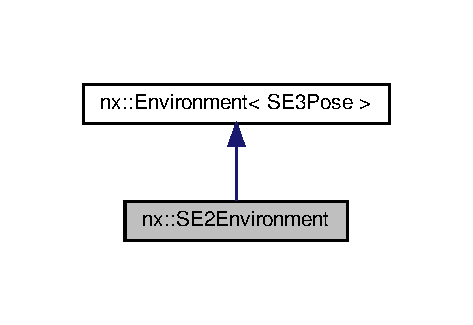
\includegraphics[width=227pt]{classnx_1_1SE2Environment__inherit__graph}
\end{center}
\end{figure}


Collaboration diagram for nx\+:\+:S\+E2\+Environment\+:
\nopagebreak
\begin{figure}[H]
\begin{center}
\leavevmode
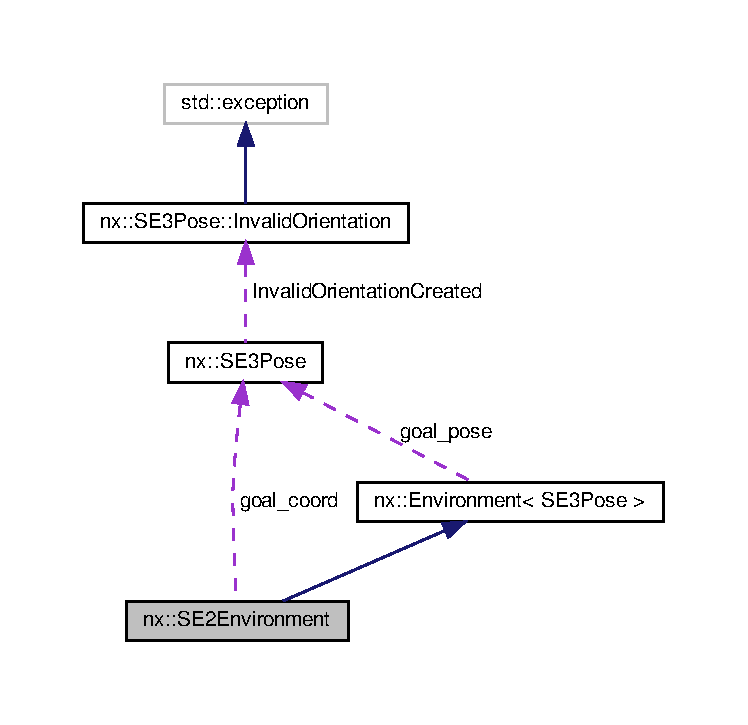
\includegraphics[width=350pt]{classnx_1_1SE2Environment__coll__graph}
\end{center}
\end{figure}
\subsection*{Public Member Functions}
\begin{DoxyCompactItemize}
\item 
\mbox{\Hypertarget{classnx_1_1SE2Environment_acbb1475684cbec971710e61cdbcadc6e}\label{classnx_1_1SE2Environment_acbb1475684cbec971710e61cdbcadc6e}} 
{\bfseries S\+E2\+Environment} (std\+::shared\+\_\+ptr$<$ \hyperlink{classnx_1_1map__nd}{nx\+::map\+\_\+nd} $>$ map\+\_\+in, std\+::shared\+\_\+ptr$<$ std\+::vector$<$ char $>$$>$ cmap\+\_\+ptr, const std\+::string \&mprim\+\_\+yaml, \hyperlink{structnx_1_1SE3Pose}{S\+E3\+Pose} goal=\hyperlink{structnx_1_1SE3Pose}{S\+E3\+Pose}())
\item 
int \hyperlink{classnx_1_1SE2Environment_a0fe7c5f438795a98f17be0ed95b2ff7c}{state\+\_\+to\+\_\+idx} (const \hyperlink{structnx_1_1SE3Pose}{S\+E3\+Pose} \&state) const override
\item 
Vector3d \hyperlink{classnx_1_1SE2Environment_ab1f9056e6fffe905ec225ee3885679b4}{state\+\_\+to\+\_\+\+S\+E2} (const \hyperlink{structnx_1_1SE3Pose}{S\+E3\+Pose} \&state) const override
\item 
std\+::vector$<$ int $>$ \hyperlink{classnx_1_1SE2Environment_ae3ac780e46d421898e3c7db696d8026f}{state\+\_\+to\+\_\+cell} (const \hyperlink{structnx_1_1SE3Pose}{S\+E3\+Pose} \&state) const override
\item 
void \hyperlink{classnx_1_1SE2Environment_a2a4159dc6bf024e522bb504c77e9aa69}{get\+\_\+succ} (const \hyperlink{structnx_1_1SE3Pose}{S\+E3\+Pose} \&curr, std\+::vector$<$ \hyperlink{structnx_1_1SE3Pose}{S\+E3\+Pose} $>$ \&succ, std\+::vector$<$ int $>$ \&succ\+\_\+idx, std\+::vector$<$ double $>$ \&succ\+\_\+cost, std\+::vector$<$ int $>$ \&action\+\_\+idx) const override
\item 
void \hyperlink{classnx_1_1SE2Environment_ac9453c2a57e53c9f511eb04aabaa0809}{forward\+\_\+action} (const \hyperlink{structnx_1_1SE3Pose}{S\+E3\+Pose} \&curr, int action\+\_\+id, std\+::vector$<$ \hyperlink{structnx_1_1SE3Pose}{S\+E3\+Pose} $>$ \&next\+\_\+micro) const override
\end{DoxyCompactItemize}
\subsection*{Protected Types}
\begin{DoxyCompactItemize}
\item 
\mbox{\Hypertarget{classnx_1_1SE2Environment_a086b171b619278b4fde9819cfb433b48}\label{classnx_1_1SE2Environment_a086b171b619278b4fde9819cfb433b48}} 
typedef \hyperlink{structnx_1_1MotionPrimitive}{Motion\+Primitive}$<$ std\+::array$<$ double, 3 $>$, std\+::array$<$ double, 2 $>$ $>$ {\bfseries M\+Prim}
\end{DoxyCompactItemize}
\subsection*{Protected Attributes}
\begin{DoxyCompactItemize}
\item 
\mbox{\Hypertarget{classnx_1_1SE2Environment_ab0c0d3623fa001720fec80fe973e551c}\label{classnx_1_1SE2Environment_ab0c0d3623fa001720fec80fe973e551c}} 
\hyperlink{structnx_1_1SE3Pose}{S\+E3\+Pose} {\bfseries goal\+\_\+coord}
\item 
\mbox{\Hypertarget{classnx_1_1SE2Environment_ae28b4b651b5b2b0f00862951083a84e6}\label{classnx_1_1SE2Environment_ae28b4b651b5b2b0f00862951083a84e6}} 
size\+\_\+t {\bfseries max\+\_\+len\+\_\+traj\+\_\+} = 0
\item 
\mbox{\Hypertarget{classnx_1_1SE2Environment_a987e1a74480013e9c7187aee9fc25820}\label{classnx_1_1SE2Environment_a987e1a74480013e9c7187aee9fc25820}} 
double {\bfseries samp} = 0.\+5
\item 
\mbox{\Hypertarget{classnx_1_1SE2Environment_a02e5b4637072bf60e4bb24fda092d166}\label{classnx_1_1SE2Environment_a02e5b4637072bf60e4bb24fda092d166}} 
int {\bfseries yaw\+\_\+discretization\+\_\+size} = 60
\item 
\mbox{\Hypertarget{classnx_1_1SE2Environment_a452850e27e78085d661707f72c72497a}\label{classnx_1_1SE2Environment_a452850e27e78085d661707f72c72497a}} 
double {\bfseries yaw\+\_\+res} = 2 $\ast$ PI / yaw\+\_\+discretization\+\_\+size
\item 
\mbox{\Hypertarget{classnx_1_1SE2Environment_a197d1b81123220efcc2b51bc7928f467}\label{classnx_1_1SE2Environment_a197d1b81123220efcc2b51bc7928f467}} 
bool {\bfseries is\+\_\+3d}
\item 
\mbox{\Hypertarget{classnx_1_1SE2Environment_a7941f5dec4704d105ce5084ce759d430}\label{classnx_1_1SE2Environment_a7941f5dec4704d105ce5084ce759d430}} 
std\+::vector$<$ std\+::vector$<$ std\+::vector$<$ std\+::vector$<$ std\+::array$<$ int, 3 $>$ $>$ $>$ $>$ $>$ {\bfseries mprim\+\_\+xd\+\_\+}
\end{DoxyCompactItemize}
\subsection*{Additional Inherited Members}


\subsection{Member Function Documentation}
\mbox{\Hypertarget{classnx_1_1SE2Environment_ac9453c2a57e53c9f511eb04aabaa0809}\label{classnx_1_1SE2Environment_ac9453c2a57e53c9f511eb04aabaa0809}} 
\index{nx\+::\+S\+E2\+Environment@{nx\+::\+S\+E2\+Environment}!forward\+\_\+action@{forward\+\_\+action}}
\index{forward\+\_\+action@{forward\+\_\+action}!nx\+::\+S\+E2\+Environment@{nx\+::\+S\+E2\+Environment}}
\subsubsection{\texorpdfstring{forward\+\_\+action()}{forward\_action()}}
{\footnotesize\ttfamily void nx\+::\+S\+E2\+Environment\+::forward\+\_\+action (\begin{DoxyParamCaption}\item[{const \hyperlink{structnx_1_1SE3Pose}{S\+E3\+Pose} \&}]{curr,  }\item[{int}]{action\+\_\+id,  }\item[{std\+::vector$<$ \hyperlink{structnx_1_1SE3Pose}{S\+E3\+Pose} $>$ \&}]{next\+\_\+micro }\end{DoxyParamCaption}) const\hspace{0.3cm}{\ttfamily [inline]}, {\ttfamily [override]}, {\ttfamily [virtual]}}

Computes the list of micro-\/states generated from applying the action with action\+\_\+id. 
\begin{DoxyParams}{Parameters}
{\em curr} & Current state. \\
\hline
{\em action\+\_\+id} & Action index to apply. \\
\hline
{\em next\+\_\+micro} & List of micro-\/states generated along the action. \\
\hline
\end{DoxyParams}


Implements \hyperlink{classnx_1_1Environment_a4f3ee5bb7665210e6262d333857e5f4f}{nx\+::\+Environment$<$ S\+E3\+Pose $>$}.

\mbox{\Hypertarget{classnx_1_1SE2Environment_a2a4159dc6bf024e522bb504c77e9aa69}\label{classnx_1_1SE2Environment_a2a4159dc6bf024e522bb504c77e9aa69}} 
\index{nx\+::\+S\+E2\+Environment@{nx\+::\+S\+E2\+Environment}!get\+\_\+succ@{get\+\_\+succ}}
\index{get\+\_\+succ@{get\+\_\+succ}!nx\+::\+S\+E2\+Environment@{nx\+::\+S\+E2\+Environment}}
\subsubsection{\texorpdfstring{get\+\_\+succ()}{get\_succ()}}
{\footnotesize\ttfamily void nx\+::\+S\+E2\+Environment\+::get\+\_\+succ (\begin{DoxyParamCaption}\item[{const \hyperlink{structnx_1_1SE3Pose}{S\+E3\+Pose} \&}]{curr,  }\item[{std\+::vector$<$ \hyperlink{structnx_1_1SE3Pose}{S\+E3\+Pose} $>$ \&}]{succ,  }\item[{std\+::vector$<$ int $>$ \&}]{succ\+\_\+idx,  }\item[{std\+::vector$<$ double $>$ \&}]{succ\+\_\+cost,  }\item[{std\+::vector$<$ int $>$ \&}]{action\+\_\+idx }\end{DoxyParamCaption}) const\hspace{0.3cm}{\ttfamily [inline]}, {\ttfamily [override]}, {\ttfamily [virtual]}}

Computes the successor nodes from state curr, taking into account the cost\+Map. 
\begin{DoxyParams}{Parameters}
{\em curr} & The current state. \\
\hline
{\em succ} & The list of successors to be computed. \\
\hline
{\em succ\+\_\+idx} & The linear indices of the successors. \\
\hline
{\em succ\+\_\+cost} & \\
\hline
{\em action\+\_\+idx} & \\
\hline
\end{DoxyParams}


Implements \hyperlink{classnx_1_1Environment_a5879e51878691196971e94880d45b551}{nx\+::\+Environment$<$ S\+E3\+Pose $>$}.

\mbox{\Hypertarget{classnx_1_1SE2Environment_ae3ac780e46d421898e3c7db696d8026f}\label{classnx_1_1SE2Environment_ae3ac780e46d421898e3c7db696d8026f}} 
\index{nx\+::\+S\+E2\+Environment@{nx\+::\+S\+E2\+Environment}!state\+\_\+to\+\_\+cell@{state\+\_\+to\+\_\+cell}}
\index{state\+\_\+to\+\_\+cell@{state\+\_\+to\+\_\+cell}!nx\+::\+S\+E2\+Environment@{nx\+::\+S\+E2\+Environment}}
\subsubsection{\texorpdfstring{state\+\_\+to\+\_\+cell()}{state\_to\_cell()}}
{\footnotesize\ttfamily std\+::vector$<$int$>$ nx\+::\+S\+E2\+Environment\+::state\+\_\+to\+\_\+cell (\begin{DoxyParamCaption}\item[{const \hyperlink{structnx_1_1SE3Pose}{S\+E3\+Pose} \&}]{ }\end{DoxyParamCaption}) const\hspace{0.3cm}{\ttfamily [inline]}, {\ttfamily [override]}, {\ttfamily [virtual]}}

Converts a state to its corresponding cell coordinates in the map. \begin{DoxyReturn}{Returns}
The cell coordinates of the state. 
\end{DoxyReturn}


Implements \hyperlink{classnx_1_1Environment_adb86237d799683c40f17c95ea39eeba3}{nx\+::\+Environment$<$ S\+E3\+Pose $>$}.

\mbox{\Hypertarget{classnx_1_1SE2Environment_a0fe7c5f438795a98f17be0ed95b2ff7c}\label{classnx_1_1SE2Environment_a0fe7c5f438795a98f17be0ed95b2ff7c}} 
\index{nx\+::\+S\+E2\+Environment@{nx\+::\+S\+E2\+Environment}!state\+\_\+to\+\_\+idx@{state\+\_\+to\+\_\+idx}}
\index{state\+\_\+to\+\_\+idx@{state\+\_\+to\+\_\+idx}!nx\+::\+S\+E2\+Environment@{nx\+::\+S\+E2\+Environment}}
\subsubsection{\texorpdfstring{state\+\_\+to\+\_\+idx()}{state\_to\_idx()}}
{\footnotesize\ttfamily int nx\+::\+S\+E2\+Environment\+::state\+\_\+to\+\_\+idx (\begin{DoxyParamCaption}\item[{const \hyperlink{structnx_1_1SE3Pose}{S\+E3\+Pose} \&}]{ }\end{DoxyParamCaption}) const\hspace{0.3cm}{\ttfamily [inline]}, {\ttfamily [override]}, {\ttfamily [virtual]}}

Converts a state to its corresponding linear index in the map. \begin{DoxyReturn}{Returns}
The linear index of the state. 
\end{DoxyReturn}


Implements \hyperlink{classnx_1_1Environment_a1c558036435de03a3afd85e940aad600}{nx\+::\+Environment$<$ S\+E3\+Pose $>$}.

\mbox{\Hypertarget{classnx_1_1SE2Environment_ab1f9056e6fffe905ec225ee3885679b4}\label{classnx_1_1SE2Environment_ab1f9056e6fffe905ec225ee3885679b4}} 
\index{nx\+::\+S\+E2\+Environment@{nx\+::\+S\+E2\+Environment}!state\+\_\+to\+\_\+\+S\+E2@{state\+\_\+to\+\_\+\+S\+E2}}
\index{state\+\_\+to\+\_\+\+S\+E2@{state\+\_\+to\+\_\+\+S\+E2}!nx\+::\+S\+E2\+Environment@{nx\+::\+S\+E2\+Environment}}
\subsubsection{\texorpdfstring{state\+\_\+to\+\_\+\+S\+E2()}{state\_to\_SE2()}}
{\footnotesize\ttfamily Vector3d nx\+::\+S\+E2\+Environment\+::state\+\_\+to\+\_\+\+S\+E2 (\begin{DoxyParamCaption}\item[{const \hyperlink{structnx_1_1SE3Pose}{S\+E3\+Pose} \&}]{ }\end{DoxyParamCaption}) const\hspace{0.3cm}{\ttfamily [inline]}, {\ttfamily [override]}, {\ttfamily [virtual]}}

Returns the pose of the state, projecected into the S\+E(2) space, i.\+e. 2.\+5D position (X,Y,Yaw). \begin{DoxyReturn}{Returns}
The S\+E(2) Pose of the state. 
\end{DoxyReturn}


Implements \hyperlink{classnx_1_1Environment_ae31bd7f19efac45fc07d405f1fcfd2b2}{nx\+::\+Environment$<$ S\+E3\+Pose $>$}.



The documentation for this class was generated from the following file\+:\begin{DoxyCompactItemize}
\item 
include/igl/env/env\+\_\+se2.\+h\end{DoxyCompactItemize}

\hypertarget{structnx_1_1SE3Pose}{}\section{nx\+:\+:S\+E3\+Pose Struct Reference}
\label{structnx_1_1SE3Pose}\index{nx\+::\+S\+E3\+Pose@{nx\+::\+S\+E3\+Pose}}


{\ttfamily \#include $<$se3\+\_\+pose.\+h$>$}



Collaboration diagram for nx\+:\+:S\+E3\+Pose\+:
\nopagebreak
\begin{figure}[H]
\begin{center}
\leavevmode
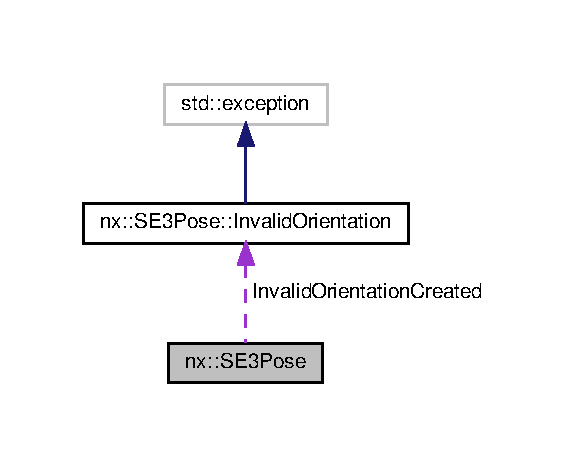
\includegraphics[width=272pt]{structnx_1_1SE3Pose__coll__graph}
\end{center}
\end{figure}
\subsection*{Classes}
\begin{DoxyCompactItemize}
\item 
class \hyperlink{classnx_1_1SE3Pose_1_1InvalidOrientation}{Invalid\+Orientation}
\end{DoxyCompactItemize}
\subsection*{Public Member Functions}
\begin{DoxyCompactItemize}
\item 
\hyperlink{structnx_1_1SE3Pose_ad53ace38f70c31c09e994404470cafc5}{S\+E3\+Pose} ()
\item 
\hyperlink{structnx_1_1SE3Pose_aedb0fbcfde8aaad17536e6401a70016f}{S\+E3\+Pose} (const Vector3d \&position, const Matrix3d \&orientation)
\item 
\hyperlink{structnx_1_1SE3Pose_a4dadedbf18209a190442ab3e5a9717da}{S\+E3\+Pose} (const Vector3d \&position, const Vector4d \&quaternion)
\item 
double \hyperlink{structnx_1_1SE3Pose_a103674ebbf5d7e62b9ead5131bbdd289}{get\+Yaw} () const
\item 
double \hyperlink{structnx_1_1SE3Pose_a98a2f187d971144630219e2f6a989f55}{get\+Pitch} () const
\item 
double \hyperlink{structnx_1_1SE3Pose_afe22fcd642b968043a5e8ef1d284ee39}{get\+Roll} () const
\item 
Vector3d \hyperlink{structnx_1_1SE3Pose_a1796e8aafcf90da2e6b0d07ca4c7135f}{get\+S\+E2} () const
\end{DoxyCompactItemize}
\subsection*{Public Attributes}
\begin{DoxyCompactItemize}
\item 
\mbox{\Hypertarget{structnx_1_1SE3Pose_a5620730d3946d81d71ba61d75653747d}\label{structnx_1_1SE3Pose_a5620730d3946d81d71ba61d75653747d}} 
\hyperlink{classnx_1_1SE3Pose_1_1InvalidOrientation}{nx\+::\+S\+E3\+Pose\+::\+Invalid\+Orientation} {\bfseries Invalid\+Orientation\+Created}
\item 
\mbox{\Hypertarget{structnx_1_1SE3Pose_a601d780745bfa4076ae444bce9360caf}\label{structnx_1_1SE3Pose_a601d780745bfa4076ae444bce9360caf}} 
Vector3d {\bfseries position} \{0, 0, 0\}
\item 
\mbox{\Hypertarget{structnx_1_1SE3Pose_a18492df5af5d735b5d21257c23bb5eca}\label{structnx_1_1SE3Pose_a18492df5af5d735b5d21257c23bb5eca}} 
Matrix3d {\bfseries orientation} \{Matrix3d\+::\+Identity()\}
\end{DoxyCompactItemize}


\subsection{Detailed Description}
S\+E3\+State stores position and orientation of a rigid body with respect to a world frame. 

\subsection{Constructor \& Destructor Documentation}
\mbox{\Hypertarget{structnx_1_1SE3Pose_ad53ace38f70c31c09e994404470cafc5}\label{structnx_1_1SE3Pose_ad53ace38f70c31c09e994404470cafc5}} 
\index{nx\+::\+S\+E3\+Pose@{nx\+::\+S\+E3\+Pose}!S\+E3\+Pose@{S\+E3\+Pose}}
\index{S\+E3\+Pose@{S\+E3\+Pose}!nx\+::\+S\+E3\+Pose@{nx\+::\+S\+E3\+Pose}}
\subsubsection{\texorpdfstring{S\+E3\+Pose()}{SE3Pose()}\hspace{0.1cm}{\footnotesize\ttfamily [1/3]}}
{\footnotesize\ttfamily nx\+::\+S\+E3\+Pose\+::\+S\+E3\+Pose (\begin{DoxyParamCaption}{ }\end{DoxyParamCaption})\hspace{0.3cm}{\ttfamily [inline]}}

Default Ctor. \mbox{\Hypertarget{structnx_1_1SE3Pose_aedb0fbcfde8aaad17536e6401a70016f}\label{structnx_1_1SE3Pose_aedb0fbcfde8aaad17536e6401a70016f}} 
\index{nx\+::\+S\+E3\+Pose@{nx\+::\+S\+E3\+Pose}!S\+E3\+Pose@{S\+E3\+Pose}}
\index{S\+E3\+Pose@{S\+E3\+Pose}!nx\+::\+S\+E3\+Pose@{nx\+::\+S\+E3\+Pose}}
\subsubsection{\texorpdfstring{S\+E3\+Pose()}{SE3Pose()}\hspace{0.1cm}{\footnotesize\ttfamily [2/3]}}
{\footnotesize\ttfamily nx\+::\+S\+E3\+Pose\+::\+S\+E3\+Pose (\begin{DoxyParamCaption}\item[{const Vector3d \&}]{position,  }\item[{const Matrix3d \&}]{orientation }\end{DoxyParamCaption})\hspace{0.3cm}{\ttfamily [inline]}}

Constructs an \hyperlink{structnx_1_1SE3Pose}{S\+E3\+Pose} from a position and orientation matrix. 
\begin{DoxyParams}{Parameters}
{\em position} & The position. \\
\hline
{\em orientation} & The orientation as a matrix. \\
\hline
\end{DoxyParams}
\mbox{\Hypertarget{structnx_1_1SE3Pose_a4dadedbf18209a190442ab3e5a9717da}\label{structnx_1_1SE3Pose_a4dadedbf18209a190442ab3e5a9717da}} 
\index{nx\+::\+S\+E3\+Pose@{nx\+::\+S\+E3\+Pose}!S\+E3\+Pose@{S\+E3\+Pose}}
\index{S\+E3\+Pose@{S\+E3\+Pose}!nx\+::\+S\+E3\+Pose@{nx\+::\+S\+E3\+Pose}}
\subsubsection{\texorpdfstring{S\+E3\+Pose()}{SE3Pose()}\hspace{0.1cm}{\footnotesize\ttfamily [3/3]}}
{\footnotesize\ttfamily nx\+::\+S\+E3\+Pose\+::\+S\+E3\+Pose (\begin{DoxyParamCaption}\item[{const Vector3d \&}]{position,  }\item[{const Vector4d \&}]{quaternion }\end{DoxyParamCaption})\hspace{0.3cm}{\ttfamily [inline]}}

Constructs an \hyperlink{structnx_1_1SE3Pose}{S\+E3\+Pose} from a position and quaternion. 
\begin{DoxyParams}{Parameters}
{\em position} & The position. \\
\hline
{\em quaternion} & The orientation as a quaternion. \\
\hline
\end{DoxyParams}


\subsection{Member Function Documentation}
\mbox{\Hypertarget{structnx_1_1SE3Pose_a98a2f187d971144630219e2f6a989f55}\label{structnx_1_1SE3Pose_a98a2f187d971144630219e2f6a989f55}} 
\index{nx\+::\+S\+E3\+Pose@{nx\+::\+S\+E3\+Pose}!get\+Pitch@{get\+Pitch}}
\index{get\+Pitch@{get\+Pitch}!nx\+::\+S\+E3\+Pose@{nx\+::\+S\+E3\+Pose}}
\subsubsection{\texorpdfstring{get\+Pitch()}{getPitch()}}
{\footnotesize\ttfamily double nx\+::\+S\+E3\+Pose\+::get\+Pitch (\begin{DoxyParamCaption}{ }\end{DoxyParamCaption}) const\hspace{0.3cm}{\ttfamily [inline]}}

Returns the Pitch of the orientation. \begin{DoxyReturn}{Returns}
The pitch. 
\end{DoxyReturn}
\mbox{\Hypertarget{structnx_1_1SE3Pose_afe22fcd642b968043a5e8ef1d284ee39}\label{structnx_1_1SE3Pose_afe22fcd642b968043a5e8ef1d284ee39}} 
\index{nx\+::\+S\+E3\+Pose@{nx\+::\+S\+E3\+Pose}!get\+Roll@{get\+Roll}}
\index{get\+Roll@{get\+Roll}!nx\+::\+S\+E3\+Pose@{nx\+::\+S\+E3\+Pose}}
\subsubsection{\texorpdfstring{get\+Roll()}{getRoll()}}
{\footnotesize\ttfamily double nx\+::\+S\+E3\+Pose\+::get\+Roll (\begin{DoxyParamCaption}{ }\end{DoxyParamCaption}) const\hspace{0.3cm}{\ttfamily [inline]}}

Returns the Roll of the orientation. \begin{DoxyReturn}{Returns}
The roll. 
\end{DoxyReturn}
\mbox{\Hypertarget{structnx_1_1SE3Pose_a1796e8aafcf90da2e6b0d07ca4c7135f}\label{structnx_1_1SE3Pose_a1796e8aafcf90da2e6b0d07ca4c7135f}} 
\index{nx\+::\+S\+E3\+Pose@{nx\+::\+S\+E3\+Pose}!get\+S\+E2@{get\+S\+E2}}
\index{get\+S\+E2@{get\+S\+E2}!nx\+::\+S\+E3\+Pose@{nx\+::\+S\+E3\+Pose}}
\subsubsection{\texorpdfstring{get\+S\+E2()}{getSE2()}}
{\footnotesize\ttfamily Vector3d nx\+::\+S\+E3\+Pose\+::get\+S\+E2 (\begin{DoxyParamCaption}{ }\end{DoxyParamCaption}) const\hspace{0.3cm}{\ttfamily [inline]}}

Returns the S\+E(2) projection of the full S\+E(3) Pose. \begin{DoxyReturn}{Returns}
The S\+E(2) pose. 
\end{DoxyReturn}
\mbox{\Hypertarget{structnx_1_1SE3Pose_a103674ebbf5d7e62b9ead5131bbdd289}\label{structnx_1_1SE3Pose_a103674ebbf5d7e62b9ead5131bbdd289}} 
\index{nx\+::\+S\+E3\+Pose@{nx\+::\+S\+E3\+Pose}!get\+Yaw@{get\+Yaw}}
\index{get\+Yaw@{get\+Yaw}!nx\+::\+S\+E3\+Pose@{nx\+::\+S\+E3\+Pose}}
\subsubsection{\texorpdfstring{get\+Yaw()}{getYaw()}}
{\footnotesize\ttfamily double nx\+::\+S\+E3\+Pose\+::get\+Yaw (\begin{DoxyParamCaption}{ }\end{DoxyParamCaption}) const\hspace{0.3cm}{\ttfamily [inline]}}

Returns the Yaw of the orientation. \begin{DoxyReturn}{Returns}
The yaw. 
\end{DoxyReturn}


The documentation for this struct was generated from the following file\+:\begin{DoxyCompactItemize}
\item 
include/igl/se3\+\_\+pose.\+h\end{DoxyCompactItemize}

\hypertarget{classnx_1_1Sensor}{}\section{nx\+:\+:Sensor$<$ state $>$ Class Template Reference}
\label{classnx_1_1Sensor}\index{nx\+::\+Sensor$<$ state $>$@{nx\+::\+Sensor$<$ state $>$}}


{\ttfamily \#include $<$sensor.\+h$>$}

\subsection*{Public Member Functions}
\begin{DoxyCompactItemize}
\item 
\mbox{\Hypertarget{classnx_1_1Sensor_a7f5218bff3e514d6539caabdbbb5e077}\label{classnx_1_1Sensor_a7f5218bff3e514d6539caabdbbb5e077}} 
{\bfseries Sensor} (int z\+\_\+dim)
\item 
virtual Vector\+Xd \hyperlink{classnx_1_1Sensor_a1dfc0088b798aa167c666f7e00587ab3}{Sense} (const state \&x, const Vector\+Xd \&target)=0
\item 
virtual std\+::vector$<$ \hyperlink{structnx_1_1Measurement}{Measurement} $>$ \hyperlink{classnx_1_1Sensor_a6c8d5300337277858d417f6279f851a7}{Sense\+Multiple} (const state \&x, const std\+::shared\+\_\+ptr$<$ \hyperlink{classnx_1_1TargetModel}{Target\+Model} $>$ \&tmm)=0
\item 
virtual void \hyperlink{classnx_1_1Sensor_aa9b370055e91f8913915d12d18450743}{Get\+Jacobian} (Matrix\+Xd \&H, Matrix\+Xd \&V, const state \&x, const std\+::shared\+\_\+ptr$<$ \hyperlink{classnx_1_1InfoTargetModel}{Info\+Target\+Model} $>$ \&tmm) const =0
\end{DoxyCompactItemize}
\subsection*{Public Attributes}
\begin{DoxyCompactItemize}
\item 
\mbox{\Hypertarget{classnx_1_1Sensor_ac6a5a70ce332694a2c7a6b5aa1dcaf1d}\label{classnx_1_1Sensor_ac6a5a70ce332694a2c7a6b5aa1dcaf1d}} 
int {\bfseries z\+\_\+dim}
\end{DoxyCompactItemize}


\subsection{Detailed Description}
\subsubsection*{template$<$class state$>$\newline
class nx\+::\+Sensor$<$ state $>$}

Generic interface for an abstract sensor type. Supports generating single measurements of a target from a state, a vector of measurements of multiple targets from a \hyperlink{classnx_1_1TargetModel}{Target\+Model}, and computation of Jacobian matrices. 

\subsection{Member Function Documentation}
\mbox{\Hypertarget{classnx_1_1Sensor_aa9b370055e91f8913915d12d18450743}\label{classnx_1_1Sensor_aa9b370055e91f8913915d12d18450743}} 
\index{nx\+::\+Sensor@{nx\+::\+Sensor}!Get\+Jacobian@{Get\+Jacobian}}
\index{Get\+Jacobian@{Get\+Jacobian}!nx\+::\+Sensor@{nx\+::\+Sensor}}
\subsubsection{\texorpdfstring{Get\+Jacobian()}{GetJacobian()}}
{\footnotesize\ttfamily template$<$class state $>$ \\
virtual void \hyperlink{classnx_1_1Sensor}{nx\+::\+Sensor}$<$ state $>$\+::Get\+Jacobian (\begin{DoxyParamCaption}\item[{Matrix\+Xd \&}]{H,  }\item[{Matrix\+Xd \&}]{V,  }\item[{const state \&}]{x,  }\item[{const std\+::shared\+\_\+ptr$<$ \hyperlink{classnx_1_1InfoTargetModel}{Info\+Target\+Model} $>$ \&}]{tmm }\end{DoxyParamCaption}) const\hspace{0.3cm}{\ttfamily [pure virtual]}}

Computes the Jacobian of the sensor measurement model. 
\begin{DoxyParams}{Parameters}
{\em H} & The Jacobian of the measurement model. \\
\hline
{\em V} & The covariance matrix. \\
\hline
{\em x} & The robot state to compute the Jacobian with respect to. \\
\hline
{\em y} & The target state to compute the Jacobian with respect to. \\
\hline
{\em y\+\_\+dim} & The dimensionality of the target, needed for correct matrix sizing. \\
\hline
\end{DoxyParams}
\mbox{\Hypertarget{classnx_1_1Sensor_a1dfc0088b798aa167c666f7e00587ab3}\label{classnx_1_1Sensor_a1dfc0088b798aa167c666f7e00587ab3}} 
\index{nx\+::\+Sensor@{nx\+::\+Sensor}!Sense@{Sense}}
\index{Sense@{Sense}!nx\+::\+Sensor@{nx\+::\+Sensor}}
\subsubsection{\texorpdfstring{Sense()}{Sense()}}
{\footnotesize\ttfamily template$<$class state $>$ \\
virtual Vector\+Xd \hyperlink{classnx_1_1Sensor}{nx\+::\+Sensor}$<$ state $>$\+::Sense (\begin{DoxyParamCaption}\item[{const state \&}]{x,  }\item[{const Vector\+Xd \&}]{target }\end{DoxyParamCaption})\hspace{0.3cm}{\ttfamily [pure virtual]}}

Computes a single measurement vector of the target from a state x. 
\begin{DoxyParams}{Parameters}
{\em x} & The state sensing from. \\
\hline
{\em target} & The target being sensed. \\
\hline
\end{DoxyParams}
\begin{DoxyReturn}{Returns}
The resulting measurement. 
\end{DoxyReturn}
\mbox{\Hypertarget{classnx_1_1Sensor_a6c8d5300337277858d417f6279f851a7}\label{classnx_1_1Sensor_a6c8d5300337277858d417f6279f851a7}} 
\index{nx\+::\+Sensor@{nx\+::\+Sensor}!Sense\+Multiple@{Sense\+Multiple}}
\index{Sense\+Multiple@{Sense\+Multiple}!nx\+::\+Sensor@{nx\+::\+Sensor}}
\subsubsection{\texorpdfstring{Sense\+Multiple()}{SenseMultiple()}}
{\footnotesize\ttfamily template$<$class state $>$ \\
virtual std\+::vector$<$\hyperlink{structnx_1_1Measurement}{Measurement}$>$ \hyperlink{classnx_1_1Sensor}{nx\+::\+Sensor}$<$ state $>$\+::Sense\+Multiple (\begin{DoxyParamCaption}\item[{const state \&}]{x,  }\item[{const std\+::shared\+\_\+ptr$<$ \hyperlink{classnx_1_1TargetModel}{Target\+Model} $>$ \&}]{tmm }\end{DoxyParamCaption})\hspace{0.3cm}{\ttfamily [pure virtual]}}

The sense function returns a vector of sensor measurements from the environment. 
\begin{DoxyParams}{Parameters}
{\em x} & The state to generate measurements from. \\
\hline
{\em tmm} & The \hyperlink{structnx_1_1Target}{Target} Model. \\
\hline
\end{DoxyParams}
\begin{DoxyReturn}{Returns}
The vector of sensor measurements generated. 
\end{DoxyReturn}


The documentation for this class was generated from the following file\+:\begin{DoxyCompactItemize}
\item 
include/igl/sensing/sensor.\+h\end{DoxyCompactItemize}

\hypertarget{structnx_1_1Parameters_1_1SystemModel}{}\section{nx\+:\+:Parameters\+:\+:System\+Model Struct Reference}
\label{structnx_1_1Parameters_1_1SystemModel}\index{nx\+::\+Parameters\+::\+System\+Model@{nx\+::\+Parameters\+::\+System\+Model}}
\subsection*{Public Attributes}
\begin{DoxyCompactItemize}
\item 
\mbox{\Hypertarget{structnx_1_1Parameters_1_1SystemModel_adc7fd68f307417b887de7e7fca6fba87}\label{structnx_1_1Parameters_1_1SystemModel_adc7fd68f307417b887de7e7fca6fba87}} 
Matrix\+Xd {\bfseries A}
\item 
\mbox{\Hypertarget{structnx_1_1Parameters_1_1SystemModel_a2b2721875cd6e914404ac4f4a1746de8}\label{structnx_1_1Parameters_1_1SystemModel_a2b2721875cd6e914404ac4f4a1746de8}} 
Matrix\+Xd {\bfseries W}
\item 
\mbox{\Hypertarget{structnx_1_1Parameters_1_1SystemModel_acbb64adfb3494c8489eeafd4975e808c}\label{structnx_1_1Parameters_1_1SystemModel_acbb64adfb3494c8489eeafd4975e808c}} 
Matrix\+Xd {\bfseries Sigma}
\end{DoxyCompactItemize}


The documentation for this struct was generated from the following file\+:\begin{DoxyCompactItemize}
\item 
include/igl/params.\+h\end{DoxyCompactItemize}

\hypertarget{structnx_1_1Target}{}\section{nx\+:\+:Target Struct Reference}
\label{structnx_1_1Target}\index{nx\+::\+Target@{nx\+::\+Target}}


{\ttfamily \#include $<$target\+\_\+model.\+h$>$}



Inheritance diagram for nx\+:\+:Target\+:
\nopagebreak
\begin{figure}[H]
\begin{center}
\leavevmode
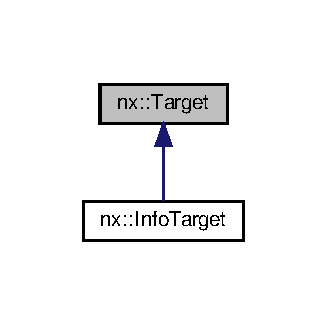
\includegraphics[width=157pt]{structnx_1_1Target__inherit__graph}
\end{center}
\end{figure}
\subsection*{Public Member Functions}
\begin{DoxyCompactItemize}
\item 
\hyperlink{structnx_1_1Target_aff71c457fa00ebbfd439d351a5574767}{Target} (int ID, const Vector\+Xd \&state, const Matrix\+Xd \&A, const Matrix\+Xd \&W)
\item 
void \hyperlink{structnx_1_1Target_a5a8c9703ee9250441895e9e7930408b0}{Update\+State} (int T)
\end{DoxyCompactItemize}
\subsection*{Public Attributes}
\begin{DoxyCompactItemize}
\item 
\mbox{\Hypertarget{structnx_1_1Target_a9f14ece231710bdf7610946ee1ad0340}\label{structnx_1_1Target_a9f14ece231710bdf7610946ee1ad0340}} 
int {\bfseries ID}
\item 
\mbox{\Hypertarget{structnx_1_1Target_ace67ce1f90bf284b8db8adad8be2ed5e}\label{structnx_1_1Target_ace67ce1f90bf284b8db8adad8be2ed5e}} 
Vector\+Xd {\bfseries state}
\item 
\mbox{\Hypertarget{structnx_1_1Target_a42f5bc317ecc3623822bb7c010b87e5a}\label{structnx_1_1Target_a42f5bc317ecc3623822bb7c010b87e5a}} 
Matrix\+Xd {\bfseries A}
\item 
\mbox{\Hypertarget{structnx_1_1Target_a8db57d5dee52aed6f2b0a2a44f034a1b}\label{structnx_1_1Target_a8db57d5dee52aed6f2b0a2a44f034a1b}} 
Matrix\+Xd {\bfseries W}
\item 
\mbox{\Hypertarget{structnx_1_1Target_af7121dba0afc6e0daa3b33a2db29d75b}\label{structnx_1_1Target_af7121dba0afc6e0daa3b33a2db29d75b}} 
int {\bfseries y\+\_\+dim}
\item 
\mbox{\Hypertarget{structnx_1_1Target_ad0147223864927924694296396478150}\label{structnx_1_1Target_ad0147223864927924694296396478150}} 
double {\bfseries max\+\_\+vel} = 1.\+0
\item 
\mbox{\Hypertarget{structnx_1_1Target_a9cebb09e697e9927429911b3eaff1dbc}\label{structnx_1_1Target_a9cebb09e697e9927429911b3eaff1dbc}} 
double {\bfseries samp} = 0.\+5
\end{DoxyCompactItemize}


\subsection{Detailed Description}
\hyperlink{structnx_1_1Target}{Target} struct describing a target with linear state evolution. 

\subsection{Constructor \& Destructor Documentation}
\mbox{\Hypertarget{structnx_1_1Target_aff71c457fa00ebbfd439d351a5574767}\label{structnx_1_1Target_aff71c457fa00ebbfd439d351a5574767}} 
\index{nx\+::\+Target@{nx\+::\+Target}!Target@{Target}}
\index{Target@{Target}!nx\+::\+Target@{nx\+::\+Target}}
\subsubsection{\texorpdfstring{Target()}{Target()}}
{\footnotesize\ttfamily nx\+::\+Target\+::\+Target (\begin{DoxyParamCaption}\item[{int}]{ID,  }\item[{const Vector\+Xd \&}]{state,  }\item[{const Matrix\+Xd \&}]{A,  }\item[{const Matrix\+Xd \&}]{W }\end{DoxyParamCaption})\hspace{0.3cm}{\ttfamily [inline]}}

Constructs a \hyperlink{structnx_1_1Target}{Target} with the following properties 
\begin{DoxyParams}{Parameters}
{\em ID} & The ID of the target. \\
\hline
{\em state} & The current state of the \hyperlink{structnx_1_1Target}{Target}. \\
\hline
{\em A} & The system dynamics matrix. \\
\hline
{\em W} & The gaussian noise matrix. \\
\hline
\end{DoxyParams}


\subsection{Member Function Documentation}
\mbox{\Hypertarget{structnx_1_1Target_a5a8c9703ee9250441895e9e7930408b0}\label{structnx_1_1Target_a5a8c9703ee9250441895e9e7930408b0}} 
\index{nx\+::\+Target@{nx\+::\+Target}!Update\+State@{Update\+State}}
\index{Update\+State@{Update\+State}!nx\+::\+Target@{nx\+::\+Target}}
\subsubsection{\texorpdfstring{Update\+State()}{UpdateState()}}
{\footnotesize\ttfamily void nx\+::\+Target\+::\+Update\+State (\begin{DoxyParamCaption}\item[{int}]{T }\end{DoxyParamCaption})\hspace{0.3cm}{\ttfamily [inline]}}

Updates the state of the \hyperlink{structnx_1_1Target}{Target} by T steps, by simulating the gaussian dynamics. 
\begin{DoxyParams}{Parameters}
{\em T} & The horizon to simulate over. \\
\hline
\end{DoxyParams}


The documentation for this struct was generated from the following file\+:\begin{DoxyCompactItemize}
\item 
include/igl/target\+\_\+motion\+\_\+models/target\+\_\+model.\+h\end{DoxyCompactItemize}

\hypertarget{classnx_1_1TargetModel}{}\section{nx\+:\+:Target\+Model Class Reference}
\label{classnx_1_1TargetModel}\index{nx\+::\+Target\+Model@{nx\+::\+Target\+Model}}


{\ttfamily \#include $<$target\+\_\+model.\+h$>$}



Inheritance diagram for nx\+:\+:Target\+Model\+:
\nopagebreak
\begin{figure}[H]
\begin{center}
\leavevmode
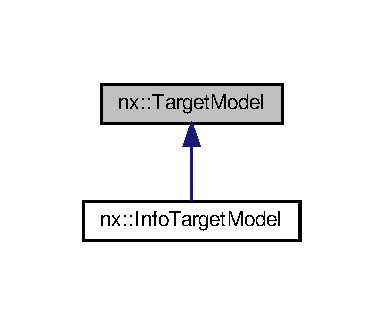
\includegraphics[width=184pt]{classnx_1_1TargetModel__inherit__graph}
\end{center}
\end{figure}
\subsection*{Public Member Functions}
\begin{DoxyCompactItemize}
\item 
\hyperlink{classnx_1_1TargetModel_ad6df134361a815092dde948c923fee87}{Target\+Model} ()
\item 
bool \hyperlink{classnx_1_1TargetModel_ab38b91d30509a7e981c456d74eecb07c}{Add\+Target} (int ID, const \hyperlink{structnx_1_1Target}{Target} \&target)
\item 
void \hyperlink{classnx_1_1TargetModel_a460f91497d1eb6808543b0bbc26ddd61}{Update\+Target} (int ID, const Vector\+Xd \&state)
\item 
void \hyperlink{classnx_1_1TargetModel_ad89e37efd10097f7c2d97f79ab380919}{Remove\+Target} (int ID)
\item 
Vector\+Xd \hyperlink{classnx_1_1TargetModel_afbdd3abdce59717ddfa16b70808178ca}{Get\+Target\+State} () const
\item 
Matrix\+Xd \hyperlink{classnx_1_1TargetModel_a1ee2990a96918171f0f779afed6d9f53}{Get\+System\+Matrix} () const
\item 
Matrix\+Xd \hyperlink{classnx_1_1TargetModel_a8b4c0bf53662bfedb955754f8debc674}{Get\+Noise\+Matrix} () const
\item 
std\+::vector$<$ Vector\+Xd $>$ \hyperlink{classnx_1_1TargetModel_a106254c8b6d05f241ab029ed7f534ea9}{Predict\+Target\+State} (int T) const
\item 
void \hyperlink{classnx_1_1TargetModel_ab170163096edacbfc2fc4e697f9cf139}{Update\+State} (int T)
\item 
int \hyperlink{classnx_1_1TargetModel_a269a926fe7a0fc4eae2416f4f0837f94}{num\+\_\+targets} () const
\end{DoxyCompactItemize}
\subsection*{Public Attributes}
\begin{DoxyCompactItemize}
\item 
\mbox{\Hypertarget{classnx_1_1TargetModel_a103cd3cc81dd956d152ef80528188ae7}\label{classnx_1_1TargetModel_a103cd3cc81dd956d152ef80528188ae7}} 
int {\bfseries target\+\_\+dim} \{0\}
\item 
\mbox{\Hypertarget{classnx_1_1TargetModel_a4e336259fa51d8c5b168256d86aea564}\label{classnx_1_1TargetModel_a4e336259fa51d8c5b168256d86aea564}} 
std\+::map$<$ int, std\+::shared\+\_\+ptr$<$ \hyperlink{structnx_1_1Target}{Target} $>$ $>$ {\bfseries targets}
\end{DoxyCompactItemize}
\subsection*{Protected Member Functions}
\begin{DoxyCompactItemize}
\item 
bool \hyperlink{classnx_1_1TargetModel_a30aa54f7e05d026d06032279855a2b14}{Add\+Shared\+Target} (int ID, std\+::shared\+\_\+ptr$<$ \hyperlink{structnx_1_1Target}{Target} $>$ target\+\_\+ptr)
\end{DoxyCompactItemize}


\subsection{Detailed Description}
Generic \hyperlink{structnx_1_1Target}{Target} Model. This model is capable of simulating the ground truth target, as well as providing Jacobians that the robot may use. 

\subsection{Constructor \& Destructor Documentation}
\mbox{\Hypertarget{classnx_1_1TargetModel_ad6df134361a815092dde948c923fee87}\label{classnx_1_1TargetModel_ad6df134361a815092dde948c923fee87}} 
\index{nx\+::\+Target\+Model@{nx\+::\+Target\+Model}!Target\+Model@{Target\+Model}}
\index{Target\+Model@{Target\+Model}!nx\+::\+Target\+Model@{nx\+::\+Target\+Model}}
\subsubsection{\texorpdfstring{Target\+Model()}{TargetModel()}}
{\footnotesize\ttfamily nx\+::\+Target\+Model\+::\+Target\+Model (\begin{DoxyParamCaption}{ }\end{DoxyParamCaption})\hspace{0.3cm}{\ttfamily [inline]}}

Constructs an empty \hyperlink{structnx_1_1Target}{Target} model. 

\subsection{Member Function Documentation}
\mbox{\Hypertarget{classnx_1_1TargetModel_a30aa54f7e05d026d06032279855a2b14}\label{classnx_1_1TargetModel_a30aa54f7e05d026d06032279855a2b14}} 
\index{nx\+::\+Target\+Model@{nx\+::\+Target\+Model}!Add\+Shared\+Target@{Add\+Shared\+Target}}
\index{Add\+Shared\+Target@{Add\+Shared\+Target}!nx\+::\+Target\+Model@{nx\+::\+Target\+Model}}
\subsubsection{\texorpdfstring{Add\+Shared\+Target()}{AddSharedTarget()}}
{\footnotesize\ttfamily bool nx\+::\+Target\+Model\+::\+Add\+Shared\+Target (\begin{DoxyParamCaption}\item[{int}]{ID,  }\item[{std\+::shared\+\_\+ptr$<$ \hyperlink{structnx_1_1Target}{Target} $>$}]{target\+\_\+ptr }\end{DoxyParamCaption})\hspace{0.3cm}{\ttfamily [inline]}, {\ttfamily [protected]}}

Underlying shared\+\_\+ptr implementation of the Add\+Target function. 
\begin{DoxyParams}{Parameters}
{\em ID} & The ID to be added. \\
\hline
{\em target\+\_\+ptr} & The shared\+\_\+ptr to the \hyperlink{structnx_1_1Target}{Target} object. \\
\hline
\end{DoxyParams}
\begin{DoxyReturn}{Returns}
The result of the Add operation. 
\end{DoxyReturn}
\mbox{\Hypertarget{classnx_1_1TargetModel_ab38b91d30509a7e981c456d74eecb07c}\label{classnx_1_1TargetModel_ab38b91d30509a7e981c456d74eecb07c}} 
\index{nx\+::\+Target\+Model@{nx\+::\+Target\+Model}!Add\+Target@{Add\+Target}}
\index{Add\+Target@{Add\+Target}!nx\+::\+Target\+Model@{nx\+::\+Target\+Model}}
\subsubsection{\texorpdfstring{Add\+Target()}{AddTarget()}}
{\footnotesize\ttfamily bool nx\+::\+Target\+Model\+::\+Add\+Target (\begin{DoxyParamCaption}\item[{int}]{ID,  }\item[{const \hyperlink{structnx_1_1Target}{Target} \&}]{target }\end{DoxyParamCaption})\hspace{0.3cm}{\ttfamily [inline]}}

Adds a target to the \hyperlink{structnx_1_1Target}{Target} Model. Returns false if a target with the same ID has been already added. 
\begin{DoxyParams}{Parameters}
{\em ID} & The ID of the target to add. \\
\hline
{\em target} & The \hyperlink{structnx_1_1Target}{Target} to be added. \\
\hline
\end{DoxyParams}
\begin{DoxyReturn}{Returns}
The result of the Add\+Target operation. 
\end{DoxyReturn}
\mbox{\Hypertarget{classnx_1_1TargetModel_a8b4c0bf53662bfedb955754f8debc674}\label{classnx_1_1TargetModel_a8b4c0bf53662bfedb955754f8debc674}} 
\index{nx\+::\+Target\+Model@{nx\+::\+Target\+Model}!Get\+Noise\+Matrix@{Get\+Noise\+Matrix}}
\index{Get\+Noise\+Matrix@{Get\+Noise\+Matrix}!nx\+::\+Target\+Model@{nx\+::\+Target\+Model}}
\subsubsection{\texorpdfstring{Get\+Noise\+Matrix()}{GetNoiseMatrix()}}
{\footnotesize\ttfamily Matrix\+Xd nx\+::\+Target\+Model\+::\+Get\+Noise\+Matrix (\begin{DoxyParamCaption}{ }\end{DoxyParamCaption}) const\hspace{0.3cm}{\ttfamily [inline]}}

Returns the joint noise matrix W of the target model. \begin{DoxyReturn}{Returns}
The noise matrix. 
\end{DoxyReturn}
\mbox{\Hypertarget{classnx_1_1TargetModel_a1ee2990a96918171f0f779afed6d9f53}\label{classnx_1_1TargetModel_a1ee2990a96918171f0f779afed6d9f53}} 
\index{nx\+::\+Target\+Model@{nx\+::\+Target\+Model}!Get\+System\+Matrix@{Get\+System\+Matrix}}
\index{Get\+System\+Matrix@{Get\+System\+Matrix}!nx\+::\+Target\+Model@{nx\+::\+Target\+Model}}
\subsubsection{\texorpdfstring{Get\+System\+Matrix()}{GetSystemMatrix()}}
{\footnotesize\ttfamily Matrix\+Xd nx\+::\+Target\+Model\+::\+Get\+System\+Matrix (\begin{DoxyParamCaption}{ }\end{DoxyParamCaption}) const\hspace{0.3cm}{\ttfamily [inline]}}

Returns the joint system matrix A of the target model. \begin{DoxyReturn}{Returns}
The system matrix. 
\end{DoxyReturn}
\mbox{\Hypertarget{classnx_1_1TargetModel_afbdd3abdce59717ddfa16b70808178ca}\label{classnx_1_1TargetModel_afbdd3abdce59717ddfa16b70808178ca}} 
\index{nx\+::\+Target\+Model@{nx\+::\+Target\+Model}!Get\+Target\+State@{Get\+Target\+State}}
\index{Get\+Target\+State@{Get\+Target\+State}!nx\+::\+Target\+Model@{nx\+::\+Target\+Model}}
\subsubsection{\texorpdfstring{Get\+Target\+State()}{GetTargetState()}}
{\footnotesize\ttfamily Vector\+Xd nx\+::\+Target\+Model\+::\+Get\+Target\+State (\begin{DoxyParamCaption}{ }\end{DoxyParamCaption}) const\hspace{0.3cm}{\ttfamily [inline]}}

Returns the joint target state as a Vector. \begin{DoxyReturn}{Returns}
The target state to be returned. 
\end{DoxyReturn}
\mbox{\Hypertarget{classnx_1_1TargetModel_a269a926fe7a0fc4eae2416f4f0837f94}\label{classnx_1_1TargetModel_a269a926fe7a0fc4eae2416f4f0837f94}} 
\index{nx\+::\+Target\+Model@{nx\+::\+Target\+Model}!num\+\_\+targets@{num\+\_\+targets}}
\index{num\+\_\+targets@{num\+\_\+targets}!nx\+::\+Target\+Model@{nx\+::\+Target\+Model}}
\subsubsection{\texorpdfstring{num\+\_\+targets()}{num\_targets()}}
{\footnotesize\ttfamily int nx\+::\+Target\+Model\+::num\+\_\+targets (\begin{DoxyParamCaption}{ }\end{DoxyParamCaption}) const\hspace{0.3cm}{\ttfamily [inline]}}

Returns the number of targets being modeled. \begin{DoxyReturn}{Returns}
Number of targets. 
\end{DoxyReturn}
\mbox{\Hypertarget{classnx_1_1TargetModel_a106254c8b6d05f241ab029ed7f534ea9}\label{classnx_1_1TargetModel_a106254c8b6d05f241ab029ed7f534ea9}} 
\index{nx\+::\+Target\+Model@{nx\+::\+Target\+Model}!Predict\+Target\+State@{Predict\+Target\+State}}
\index{Predict\+Target\+State@{Predict\+Target\+State}!nx\+::\+Target\+Model@{nx\+::\+Target\+Model}}
\subsubsection{\texorpdfstring{Predict\+Target\+State()}{PredictTargetState()}}
{\footnotesize\ttfamily std\+::vector$<$Vector\+Xd$>$ nx\+::\+Target\+Model\+::\+Predict\+Target\+State (\begin{DoxyParamCaption}\item[{int}]{T }\end{DoxyParamCaption}) const\hspace{0.3cm}{\ttfamily [inline]}}

Predicts a target trajectory of horizon T, and returns the result. The first entry is the current state. 
\begin{DoxyParams}{Parameters}
{\em T} & The time horizon to predict the trajectory over. \\
\hline
\end{DoxyParams}
\begin{DoxyReturn}{Returns}
The vector of predicted target states over the horizon. 
\end{DoxyReturn}
\mbox{\Hypertarget{classnx_1_1TargetModel_ad89e37efd10097f7c2d97f79ab380919}\label{classnx_1_1TargetModel_ad89e37efd10097f7c2d97f79ab380919}} 
\index{nx\+::\+Target\+Model@{nx\+::\+Target\+Model}!Remove\+Target@{Remove\+Target}}
\index{Remove\+Target@{Remove\+Target}!nx\+::\+Target\+Model@{nx\+::\+Target\+Model}}
\subsubsection{\texorpdfstring{Remove\+Target()}{RemoveTarget()}}
{\footnotesize\ttfamily void nx\+::\+Target\+Model\+::\+Remove\+Target (\begin{DoxyParamCaption}\item[{int}]{ID }\end{DoxyParamCaption})\hspace{0.3cm}{\ttfamily [inline]}}

Removes a target with the ID specified. 
\begin{DoxyParams}{Parameters}
{\em ID} & The ID to be removed from the target set. \\
\hline
\end{DoxyParams}
\mbox{\Hypertarget{classnx_1_1TargetModel_ab170163096edacbfc2fc4e697f9cf139}\label{classnx_1_1TargetModel_ab170163096edacbfc2fc4e697f9cf139}} 
\index{nx\+::\+Target\+Model@{nx\+::\+Target\+Model}!Update\+State@{Update\+State}}
\index{Update\+State@{Update\+State}!nx\+::\+Target\+Model@{nx\+::\+Target\+Model}}
\subsubsection{\texorpdfstring{Update\+State()}{UpdateState()}}
{\footnotesize\ttfamily void nx\+::\+Target\+Model\+::\+Update\+State (\begin{DoxyParamCaption}\item[{int}]{T }\end{DoxyParamCaption})\hspace{0.3cm}{\ttfamily [inline]}}

Updates the state of all targets by simulating the gaussian system model. 
\begin{DoxyParams}{Parameters}
{\em T} & The number of timesteps to evolve the environment by. \\
\hline
\end{DoxyParams}
\mbox{\Hypertarget{classnx_1_1TargetModel_a460f91497d1eb6808543b0bbc26ddd61}\label{classnx_1_1TargetModel_a460f91497d1eb6808543b0bbc26ddd61}} 
\index{nx\+::\+Target\+Model@{nx\+::\+Target\+Model}!Update\+Target@{Update\+Target}}
\index{Update\+Target@{Update\+Target}!nx\+::\+Target\+Model@{nx\+::\+Target\+Model}}
\subsubsection{\texorpdfstring{Update\+Target()}{UpdateTarget()}}
{\footnotesize\ttfamily void nx\+::\+Target\+Model\+::\+Update\+Target (\begin{DoxyParamCaption}\item[{int}]{ID,  }\item[{const Vector\+Xd \&}]{state }\end{DoxyParamCaption})\hspace{0.3cm}{\ttfamily [inline]}}

Updates the state of the target with specified ID. Does nothing if the target does not exist. 
\begin{DoxyParams}{Parameters}
{\em ID} & The ID of the target to be updated. \\
\hline
{\em state} & The new state to be updated. \\
\hline
\end{DoxyParams}


The documentation for this class was generated from the following file\+:\begin{DoxyCompactItemize}
\item 
include/igl/target\+\_\+motion\+\_\+models/target\+\_\+model.\+h\end{DoxyCompactItemize}

%--- End generated contents ---

% Index
\backmatter
\newpage
\phantomsection
\clearemptydoublepage
\addcontentsline{toc}{chapter}{Index}
\printindex

\end{document}
